\documentclass[a4paper]{book}
\usepackage{makeidx}
\usepackage{graphicx}
\usepackage{multicol}
\usepackage{float}
\usepackage{listings}
\usepackage{color}
\usepackage{textcomp}
\usepackage{alltt}
\usepackage{times}
\usepackage{ifpdf}
\ifpdf
\usepackage[pdftex,
            pagebackref=true,
            colorlinks=true,
            linkcolor=blue,
            unicode
           ]{hyperref}
\else
\usepackage[ps2pdf,
            pagebackref=true,
            colorlinks=true,
            linkcolor=blue,
            unicode
           ]{hyperref}
\usepackage{pspicture}
\fi
\usepackage[utf8]{inputenc}
\usepackage{doxygen}
\lstset{language=C++,inputencoding=utf8,basicstyle=\footnotesize,breaklines=true,breakatwhitespace=true,tabsize=8,numbers=left }
\makeindex
\setcounter{tocdepth}{3}
\renewcommand{\footrulewidth}{0.4pt}
\begin{document}
\hypersetup{pageanchor=false}
\begin{titlepage}
\vspace*{7cm}
\begin{center}
{\Large math }\\
\vspace*{1cm}
{\large Generated by Doxygen 1.6.1}\\
\vspace*{0.5cm}
{\small Thu Apr 24 09:37:31 2014}\\
\end{center}
\end{titlepage}
\clearemptydoublepage
\pagenumbering{roman}
\tableofcontents
\clearemptydoublepage
\pagenumbering{arabic}
\hypersetup{pageanchor=true}
\chapter{Todo List}
\label{todo}
\hypertarget{todo}{}
\label{todo__todo000001}
\hypertarget{todo__todo000001}{}
 
\begin{DoxyDescription}
\item[Namespace \hyperlink{namespacemath_1_1geo}{math::geo} ]use these classes in the \hyperlink{classvclip}{vclip} algorithm 
\end{DoxyDescription}
\chapter{Namespace Index}
\section{Namespace List}
Here is a list of all documented namespaces with brief descriptions:\begin{DoxyCompactList}
\item\contentsline{section}{\hyperlink{namespacemath}{math} (the math library )}{\pageref{namespacemath}}{}
\item\contentsline{section}{\hyperlink{namespacemath_1_1except}{math::except} (Exceptions )}{\pageref{namespacemath_1_1except}}{}
\item\contentsline{section}{\hyperlink{namespacemath_1_1geo}{math::geo} (Geometry )}{\pageref{namespacemath_1_1geo}}{}
\item\contentsline{section}{\hyperlink{namespacemath_1_1vclip}{math::vclip} (vclip )}{\pageref{namespacemath_1_1vclip}}{}
\end{DoxyCompactList}

\chapter{Class Index}
\section{Class Hierarchy}
This inheritance list is sorted roughly, but not completely, alphabetically:\begin{DoxyCompactList}
\item \contentsline{section}{array$<$ T, D $>$}{\pageref{classarray}}{}
\item \contentsline{section}{math::color$<$ T $>$}{\pageref{classmath_1_1color}}{}
\item \contentsline{section}{math::except::domain}{\pageref{classmath_1_1except_1_1domain}}{}
\item \contentsline{section}{math::discrete::Graph::Edge}{\pageref{classmath_1_1discrete_1_1Graph_1_1Edge}}{}
\begin{DoxyCompactList}
\item \contentsline{section}{math::discrete::Graph::EdgeWeighted}{\pageref{classmath_1_1discrete_1_1Graph_1_1EdgeWeighted}}{}
\end{DoxyCompactList}
\item \contentsline{section}{feature}{\pageref{classfeature}}{}
\begin{DoxyCompactList}
\item \contentsline{section}{edge}{\pageref{classedge}}{}
\item \contentsline{section}{face}{\pageref{classface}}{}
\item \contentsline{section}{vertex}{\pageref{classvertex}}{}
\end{DoxyCompactList}
\item \contentsline{section}{math::discrete::Graph::Graph}{\pageref{classmath_1_1discrete_1_1Graph_1_1Graph}}{}
\item \contentsline{section}{math::geo::height\_\-map}{\pageref{classmath_1_1geo_1_1height__map}}{}
\item \contentsline{section}{math::discrete::Graph::Node}{\pageref{classmath_1_1discrete_1_1Graph_1_1Node}}{}
\item \contentsline{section}{math::plane}{\pageref{classmath_1_1plane}}{}
\item \contentsline{section}{plane}{\pageref{classplane}}{}
\item \contentsline{section}{math::geo::polygon}{\pageref{classmath_1_1geo_1_1polygon}}{}
\item \contentsline{section}{polyhedron}{\pageref{classpolyhedron}}{}
\item \contentsline{section}{math::geo::polyhedron}{\pageref{classmath_1_1geo_1_1polyhedron}}{}
\begin{DoxyCompactList}
\item \contentsline{section}{math::geo::polyhedron\_\-convex}{\pageref{classmath_1_1geo_1_1polyhedron__convex}}{}
\begin{DoxyCompactList}
\item \contentsline{section}{math::geo::cuboid}{\pageref{classmath_1_1geo_1_1cuboid}}{}
\item \contentsline{section}{math::geo::sphere}{\pageref{classmath_1_1geo_1_1sphere}}{}
\item \contentsline{section}{math::geo::tetrahedron}{\pageref{classmath_1_1geo_1_1tetrahedron}}{}
\item \contentsline{section}{math::geo::wedge}{\pageref{classmath_1_1geo_1_1wedge}}{}
\end{DoxyCompactList}
\end{DoxyCompactList}
\item \contentsline{section}{math::polynomial}{\pageref{classmath_1_1polynomial}}{}
\item \contentsline{section}{math::geo::quad}{\pageref{classmath_1_1geo_1_1quad}}{}
\item \contentsline{section}{math::quat$<$ T $>$}{\pageref{classmath_1_1quat}}{}
\item \contentsline{section}{math::transform$<$ T $>$}{\pageref{classmath_1_1transform}}{}
\item \contentsline{section}{math::geo::tri}{\pageref{classmath_1_1geo_1_1tri}}{}
\item \contentsline{section}{math::color$<$ T $>$::type}{\pageref{structmath_1_1color_1_1type}}{}
\item \contentsline{section}{vclip}{\pageref{classvclip}}{}
\item \contentsline{section}{math::vec2}{\pageref{classmath_1_1vec2}}{}
\item \contentsline{section}{math::vecbase$<$ T, N $>$}{\pageref{classmath_1_1vecbase}}{}
\begin{DoxyCompactList}
\item \contentsline{section}{math::matbase$<$ T, N, N $>$}{\pageref{classmath_1_1matbase}}{}
\begin{DoxyCompactList}
\item \contentsline{section}{math::matsqu$<$ T, N $>$}{\pageref{classmath_1_1matsqu}}{}
\end{DoxyCompactList}
\end{DoxyCompactList}
\item \contentsline{section}{math::vecbase$<$ T, 3 $>$}{\pageref{classmath_1_1vecbase}}{}
\begin{DoxyCompactList}
\item \contentsline{section}{math::vec3$<$ T $>$}{\pageref{classmath_1_1vec3}}{}
\end{DoxyCompactList}
\item \contentsline{section}{math::vecbase$<$ T, 4 $>$}{\pageref{classmath_1_1vecbase}}{}
\begin{DoxyCompactList}
\item \contentsline{section}{math::vec4$<$ T $>$}{\pageref{classmath_1_1vec4}}{}
\end{DoxyCompactList}
\item \contentsline{section}{math::vecbase$<$ T, 9 $>$}{\pageref{classmath_1_1vecbase}}{}
\begin{DoxyCompactList}
\item \contentsline{section}{math::mat33$<$ T $>$}{\pageref{classmath_1_1mat33}}{}
\end{DoxyCompactList}
\item \contentsline{section}{math::vecbase$<$ T, R $\ast$C $>$}{\pageref{classmath_1_1vecbase}}{}
\begin{DoxyCompactList}
\item \contentsline{section}{math::matbase$<$ T, R, C $>$}{\pageref{classmath_1_1matbase}}{}
\begin{DoxyCompactList}
\item \contentsline{section}{math::matsqu$<$ T, 4 $>$}{\pageref{classmath_1_1matsqu}}{}
\begin{DoxyCompactList}
\item \contentsline{section}{math::mat44$<$ T $>$}{\pageref{classmath_1_1mat44}}{}
\end{DoxyCompactList}
\end{DoxyCompactList}
\end{DoxyCompactList}
\item \contentsline{section}{math::geo::vertex}{\pageref{classmath_1_1geo_1_1vertex}}{}
\end{DoxyCompactList}

\chapter{Class Index}
\section{Class List}
Here are the classes, structs, unions and interfaces with brief descriptions:\begin{DoxyCompactList}
\item\contentsline{section}{\hyperlink{classarray}{array$<$ T, D $>$} }{\pageref{classarray}}{}
\item\contentsline{section}{\hyperlink{classmath_1_1color}{math::color$<$ T $>$} }{\pageref{classmath_1_1color}}{}
\item\contentsline{section}{\hyperlink{classmath_1_1geo_1_1cuboid}{math::geo::cuboid} }{\pageref{classmath_1_1geo_1_1cuboid}}{}
\item\contentsline{section}{\hyperlink{classmath_1_1except_1_1domain}{math::except::domain} }{\pageref{classmath_1_1except_1_1domain}}{}
\item\contentsline{section}{\hyperlink{classmath_1_1discrete_1_1Graph_1_1Edge}{math::discrete::Graph::Edge} }{\pageref{classmath_1_1discrete_1_1Graph_1_1Edge}}{}
\item\contentsline{section}{\hyperlink{classedge}{edge} }{\pageref{classedge}}{}
\item\contentsline{section}{\hyperlink{classmath_1_1discrete_1_1Graph_1_1EdgeWeighted}{math::discrete::Graph::EdgeWeighted} }{\pageref{classmath_1_1discrete_1_1Graph_1_1EdgeWeighted}}{}
\item\contentsline{section}{\hyperlink{classface}{face} }{\pageref{classface}}{}
\item\contentsline{section}{\hyperlink{classfeature}{feature} }{\pageref{classfeature}}{}
\item\contentsline{section}{\hyperlink{classmath_1_1discrete_1_1Graph_1_1Graph}{math::discrete::Graph::Graph} }{\pageref{classmath_1_1discrete_1_1Graph_1_1Graph}}{}
\item\contentsline{section}{\hyperlink{classmath_1_1geo_1_1height__map}{math::geo::height\_\-map} }{\pageref{classmath_1_1geo_1_1height__map}}{}
\item\contentsline{section}{\hyperlink{classmath_1_1mat33}{math::mat33$<$ T $>$} }{\pageref{classmath_1_1mat33}}{}
\item\contentsline{section}{\hyperlink{classmath_1_1mat44}{math::mat44$<$ T $>$} }{\pageref{classmath_1_1mat44}}{}
\item\contentsline{section}{\hyperlink{classmath_1_1matbase}{math::matbase$<$ T, R, C $>$} }{\pageref{classmath_1_1matbase}}{}
\item\contentsline{section}{\hyperlink{classmath_1_1matsqu}{math::matsqu$<$ T, N $>$} }{\pageref{classmath_1_1matsqu}}{}
\item\contentsline{section}{\hyperlink{classmath_1_1discrete_1_1Graph_1_1Node}{math::discrete::Graph::Node} }{\pageref{classmath_1_1discrete_1_1Graph_1_1Node}}{}
\item\contentsline{section}{\hyperlink{classmath_1_1plane}{math::plane$<$ T $>$} }{\pageref{classmath_1_1plane}}{}
\item\contentsline{section}{\hyperlink{classplane}{plane} }{\pageref{classplane}}{}
\item\contentsline{section}{\hyperlink{classmath_1_1geo_1_1polygon}{math::geo::polygon} }{\pageref{classmath_1_1geo_1_1polygon}}{}
\item\contentsline{section}{\hyperlink{classpolyhedron}{polyhedron} }{\pageref{classpolyhedron}}{}
\item\contentsline{section}{\hyperlink{classmath_1_1geo_1_1polyhedron}{math::geo::polyhedron} }{\pageref{classmath_1_1geo_1_1polyhedron}}{}
\item\contentsline{section}{\hyperlink{classmath_1_1geo_1_1polyhedron__convex}{math::geo::polyhedron\_\-convex} }{\pageref{classmath_1_1geo_1_1polyhedron__convex}}{}
\item\contentsline{section}{\hyperlink{classmath_1_1polynomial}{math::polynomial} }{\pageref{classmath_1_1polynomial}}{}
\item\contentsline{section}{\hyperlink{classmath_1_1geo_1_1quad}{math::geo::quad} }{\pageref{classmath_1_1geo_1_1quad}}{}
\item\contentsline{section}{\hyperlink{classmath_1_1quat}{math::quat$<$ T $>$} }{\pageref{classmath_1_1quat}}{}
\item\contentsline{section}{\hyperlink{classmath_1_1geo_1_1sphere}{math::geo::sphere} }{\pageref{classmath_1_1geo_1_1sphere}}{}
\item\contentsline{section}{\hyperlink{classmath_1_1geo_1_1tetrahedron}{math::geo::tetrahedron} }{\pageref{classmath_1_1geo_1_1tetrahedron}}{}
\item\contentsline{section}{\hyperlink{classmath_1_1transform}{math::transform$<$ T $>$} }{\pageref{classmath_1_1transform}}{}
\item\contentsline{section}{\hyperlink{classmath_1_1geo_1_1tri}{math::geo::tri} }{\pageref{classmath_1_1geo_1_1tri}}{}
\item\contentsline{section}{\hyperlink{structmath_1_1color_1_1type}{math::color$<$ T $>$::type} }{\pageref{structmath_1_1color_1_1type}}{}
\item\contentsline{section}{\hyperlink{classvclip}{vclip} }{\pageref{classvclip}}{}
\item\contentsline{section}{\hyperlink{classmath_1_1vec2}{math::vec2} }{\pageref{classmath_1_1vec2}}{}
\item\contentsline{section}{\hyperlink{classmath_1_1vec3}{math::vec3$<$ T $>$} }{\pageref{classmath_1_1vec3}}{}
\item\contentsline{section}{\hyperlink{classmath_1_1vec4}{math::vec4$<$ T $>$} }{\pageref{classmath_1_1vec4}}{}
\item\contentsline{section}{\hyperlink{classmath_1_1vecbase}{math::vecbase$<$ T, N $>$} }{\pageref{classmath_1_1vecbase}}{}
\item\contentsline{section}{\hyperlink{classvertex}{vertex} }{\pageref{classvertex}}{}
\item\contentsline{section}{\hyperlink{classmath_1_1geo_1_1vertex}{math::geo::vertex} }{\pageref{classmath_1_1geo_1_1vertex}}{}
\item\contentsline{section}{\hyperlink{classmath_1_1geo_1_1wedge}{math::geo::wedge} }{\pageref{classmath_1_1geo_1_1wedge}}{}
\end{DoxyCompactList}

\chapter{Namespace Documentation}
\hypertarget{namespacemath}{
\section{math Namespace Reference}
\label{namespacemath}\index{math@{math}}
}


the math library  
\subsection*{Namespaces}
\begin{DoxyCompactItemize}
\item 
namespace \hyperlink{namespacemath_1_1except}{except}


\begin{DoxyCompactList}\small\item\em exceptions \item\end{DoxyCompactList}\end{DoxyCompactItemize}
\subsection*{Classes}
\begin{DoxyCompactItemize}
\item 
class \hyperlink{classmath_1_1color}{color}
\item 
class \hyperlink{classmath_1_1mat33}{mat33}
\item 
class \hyperlink{classmath_1_1mat44}{mat44}
\item 
class \hyperlink{classmath_1_1plane}{plane}
\item 
class \hyperlink{classmath_1_1polynomial}{polynomial}
\item 
class \hyperlink{classmath_1_1quat}{quat}
\item 
class \hyperlink{classmath_1_1transform}{transform}
\item 
class \hyperlink{classmath_1_1vec2}{vec2}
\item 
class \hyperlink{classmath_1_1vec3}{vec3}
\item 
class \hyperlink{classmath_1_1vec4}{vec4}
\item 
class \hyperlink{classmath_1_1vecbase}{vecbase}
\item 
class \hyperlink{classmath_1_1matbase}{matbase}
\item 
class \hyperlink{classmath_1_1matsqu}{matsqu}
\end{DoxyCompactItemize}
\subsection*{Functions}
\begin{DoxyCompactItemize}
\item 
\hypertarget{namespacemath_a5152623417b213edfe5844fc9dad4611}{
const \hyperlink{classmath_1_1color}{color} {\bfseries white} (1.0f, 1.0f, 1.0f, 1.0f)}
\label{namespacemath_a5152623417b213edfe5844fc9dad4611}

\item 
\hypertarget{namespacemath_a9622427e2eecf89d4b0f9e661947e016}{
const \hyperlink{classmath_1_1color}{color} {\bfseries black} (0.0f, 0.0f, 0.0f, 1.0f)}
\label{namespacemath_a9622427e2eecf89d4b0f9e661947e016}

\item 
\hypertarget{namespacemath_a9fc9176d50292de598bcc7c0655ea8cb}{
const \hyperlink{classmath_1_1color}{color} {\bfseries red} (1.0f, 0.0f, 0.0f, 1.0f)}
\label{namespacemath_a9fc9176d50292de598bcc7c0655ea8cb}

\item 
\hypertarget{namespacemath_a42866786f5b1a09a9e51499ef1c4e8a9}{
const \hyperlink{classmath_1_1color}{color} {\bfseries green} (0.0f, 1.0f, 0.0f, 1.0f)}
\label{namespacemath_a42866786f5b1a09a9e51499ef1c4e8a9}

\item 
\hypertarget{namespacemath_aeb13f0bfedf6fe91be02291269f63115}{
const \hyperlink{classmath_1_1color}{color} {\bfseries blue} (0.0f, 0.0f, 1.0f, 1.0f)}
\label{namespacemath_aeb13f0bfedf6fe91be02291269f63115}

\item 
\hypertarget{namespacemath_a285692bb5482b41bc47464476d2a6cda}{
const \hyperlink{classmath_1_1color}{color} {\bfseries cyan} (0.0f, 1.0f, 1.0f, 1.0f)}
\label{namespacemath_a285692bb5482b41bc47464476d2a6cda}

\item 
\hypertarget{namespacemath_a395028a3f71934c4a6b5174c9cc6d809}{
const \hyperlink{classmath_1_1color}{color} {\bfseries magenta} (1.0f, 0.0f, 1.0f, 1.0f)}
\label{namespacemath_a395028a3f71934c4a6b5174c9cc6d809}

\item 
\hypertarget{namespacemath_a22ff1288b7db758d7dbabded48a340e9}{
const \hyperlink{classmath_1_1color}{color} {\bfseries yellow} (1.0f, 1.0f, 0.0f, 1.0f)}
\label{namespacemath_a22ff1288b7db758d7dbabded48a340e9}

\item 
\hypertarget{namespacemath_a33ac1b1153a2dcbc471ea6a4a7a06454}{
\hyperlink{classmath_1_1quat}{quat} {\bfseries slerp} (\hyperlink{classmath_1_1quat}{quat}, \hyperlink{classmath_1_1quat}{quat}, float)}
\label{namespacemath_a33ac1b1153a2dcbc471ea6a4a7a06454}

\item 
\hypertarget{namespacemath_aab0f4b6e5450449993509452ec3f5346}{
float {\bfseries recipsqrt} (float const \&)}
\label{namespacemath_aab0f4b6e5450449993509452ec3f5346}

\item 
\hypertarget{namespacemath_ae4ed1a3349ed01004dec19f19339135e}{
void {\bfseries hexdump} (void $\ast$, size\_\-t)}
\label{namespacemath_ae4ed1a3349ed01004dec19f19339135e}

\item 
\hypertarget{namespacemath_a41c77dfe60e0610f09beaca0bfaecca5}{
\hyperlink{classmath_1_1mat44}{mat44} {\bfseries perspective} (float fovy, float aspect, float zn, float zf)}
\label{namespacemath_a41c77dfe60e0610f09beaca0bfaecca5}

\item 
\hypertarget{namespacemath_ae24b1d47e947a21a2677c89b8ef0ea23}{
\hyperlink{classmath_1_1mat44}{mat44} {\bfseries lookat} (\hyperlink{classmath_1_1vec3}{math::vec3} eye, \hyperlink{classmath_1_1vec3}{math::vec3} center, \hyperlink{classmath_1_1vec3}{math::vec3} up)}
\label{namespacemath_ae24b1d47e947a21a2677c89b8ef0ea23}

\end{DoxyCompactItemize}


\subsection{Detailed Description}
the math library 
\hypertarget{namespacemath_1_1except}{
\section{math::except Namespace Reference}
\label{namespacemath_1_1except}\index{math::except@{math::except}}
}


Exceptions  
\subsection*{Classes}
\begin{DoxyCompactItemize}
\item 
class \hyperlink{classmath_1_1except_1_1domain}{domain}
\end{DoxyCompactItemize}


\subsection{Detailed Description}
Exceptions 
\hypertarget{namespacemath_1_1geo}{
\section{math::geo Namespace Reference}
\label{namespacemath_1_1geo}\index{math::geo@{math::geo}}
}


Geometry  
\subsection*{Classes}
\begin{DoxyCompactItemize}
\item 
class \hyperlink{classmath_1_1geo_1_1height__map}{height\_\-map}
\item 
class \hyperlink{classmath_1_1geo_1_1vertex}{vertex}
\item 
class \hyperlink{classmath_1_1geo_1_1polygon}{polygon}
\item 
class \hyperlink{classmath_1_1geo_1_1tri}{tri}
\item 
class \hyperlink{classmath_1_1geo_1_1quad}{quad}
\item 
class \hyperlink{classmath_1_1geo_1_1polyhedron}{polyhedron}
\item 
class \hyperlink{classmath_1_1geo_1_1polyhedron__convex}{polyhedron\_\-convex}
\item 
class \hyperlink{classmath_1_1geo_1_1sphere}{sphere}
\item 
class \hyperlink{classmath_1_1geo_1_1wedge}{wedge}
\item 
class \hyperlink{classmath_1_1geo_1_1tetrahedron}{tetrahedron}
\item 
class \hyperlink{classmath_1_1geo_1_1cuboid}{cuboid}
\end{DoxyCompactItemize}


\subsection{Detailed Description}
Geometry class for the construction of polyhedrons

\begin{Desc}
\item[\hyperlink{todo__todo000001}{Todo}]use these classes in the \hyperlink{namespacemath_1_1vclip}{vclip} algorithm \end{Desc}

\hypertarget{namespacemath_1_1vclip}{
\section{math::vclip Namespace Reference}
\label{namespacemath_1_1vclip}\index{math::vclip@{math::vclip}}
}


vclip  


\subsection{Detailed Description}
vclip \hyperlink{namespacemath_1_1vclip}{vclip} algorithm for convex polygon collision detection 
\chapter{Class Documentation}
\hypertarget{classarray}{
\section{array$<$ T, D $>$ Class Template Reference}
\label{classarray}\index{array@{array}}
}
\subsection*{Public Member Functions}
\begin{DoxyCompactItemize}
\item 
\hypertarget{classarray_ab3491a5460b213451b0837fe7d417946}{
void {\bfseries alloc\_\-sub} (int \&a, int s)}
\label{classarray_ab3491a5460b213451b0837fe7d417946}

\item 
\hypertarget{classarray_ae3794543c52e3063061923099264a441}{
{\footnotesize template$<$typename... S$>$ }\\void {\bfseries zeros} (S...s)}
\label{classarray_ae3794543c52e3063061923099264a441}

\item 
\hypertarget{classarray_a155d85b8477bedf8379e29288f96bb12}{
void {\bfseries alloc} (int const $\ast$s)}
\label{classarray_a155d85b8477bedf8379e29288f96bb12}

\item 
\hypertarget{classarray_a7da487ddfe99bc1cdcd26eff9efc2013}{
{\footnotesize template$<$typename... S$>$ }\\void {\bfseries alloc} (S...s)}
\label{classarray_a7da487ddfe99bc1cdcd26eff9efc2013}

\item 
\hypertarget{classarray_a6edd94a7b183b1c219e0fdccf54af80f}{
void {\bfseries at\_\-sub} (int $\ast$i, int \&a, int s)}
\label{classarray_a6edd94a7b183b1c219e0fdccf54af80f}

\item 
\hypertarget{classarray_a55da36dbe002fd18f88b64bf6f6f14e8}{
{\footnotesize template$<$int... S$>$ }\\T \& {\bfseries at} ()}
\label{classarray_a55da36dbe002fd18f88b64bf6f6f14e8}

\item 
\hypertarget{classarray_a217bd29d6caea27260c4ee44afec94d0}{
T \& {\bfseries at} (int $\ast$i)}
\label{classarray_a217bd29d6caea27260c4ee44afec94d0}

\item 
\hypertarget{classarray_af7085f3c6bc7aa77f4c69dc106f20f03}{
void {\bfseries print\_\-sub} (char const $\ast$fmt, int $\ast$i, int lvl)}
\label{classarray_af7085f3c6bc7aa77f4c69dc106f20f03}

\item 
\hypertarget{classarray_ae6ce8cec926e8422a243f9d189296265}{
\hyperlink{classarray}{array}$<$ T, D $>$ \& {\bfseries operator=} (\hyperlink{classarray}{array}$<$ T, D $>$ const \&rhs)}
\label{classarray_ae6ce8cec926e8422a243f9d189296265}

\item 
\hypertarget{classarray_af1ee5ea8e9a153ffc26a513e442916a1}{
\hyperlink{classarray}{array}$<$ T, D $>$ \& {\bfseries operator+=} (\hyperlink{classarray}{array}$<$ T, D $>$ const \&rhs)}
\label{classarray_af1ee5ea8e9a153ffc26a513e442916a1}

\item 
\hypertarget{classarray_a707d31f0cd68cf8c29578ceeffd4f160}{
\hyperlink{classarray}{array}$<$ T, D $>$ \& {\bfseries operator+=} (T const \&rhs)}
\label{classarray_a707d31f0cd68cf8c29578ceeffd4f160}

\item 
\hypertarget{classarray_ad2d3f9c01dd2e53e0575f25d99fa5332}{
\hyperlink{classarray}{array}$<$ T, D $>$ {\bfseries operator+} (\hyperlink{classarray}{array}$<$ T, D $>$ const \&rhs)}
\label{classarray_ad2d3f9c01dd2e53e0575f25d99fa5332}

\item 
\hypertarget{classarray_aa8116676705ae21a643f3fa6fbfc8d16}{
\hyperlink{classarray}{array}$<$ T, D $>$ {\bfseries operator+} (T const \&rhs)}
\label{classarray_aa8116676705ae21a643f3fa6fbfc8d16}

\item 
\hypertarget{classarray_afaaffd8caa1ff3e9b0c676bce63b4620}{
void {\bfseries print} (char const $\ast$fmt)}
\label{classarray_afaaffd8caa1ff3e9b0c676bce63b4620}

\end{DoxyCompactItemize}
\subsection*{Public Attributes}
\begin{DoxyCompactItemize}
\item 
\hypertarget{classarray_a26bbf20751fa00968b42384186ffa1f0}{
int {\bfseries shape} \mbox{[}D\mbox{]}}
\label{classarray_a26bbf20751fa00968b42384186ffa1f0}

\item 
\hypertarget{classarray_aece99778954bbd58c36a3ca2a1eb6122}{
int {\bfseries size}}
\label{classarray_aece99778954bbd58c36a3ca2a1eb6122}

\item 
\hypertarget{classarray_ac0f2991b5e69fca9e7b8882b6910492a}{
T $\ast$ {\bfseries v}}
\label{classarray_ac0f2991b5e69fca9e7b8882b6910492a}

\end{DoxyCompactItemize}
\subsubsection*{template$<$typename T = double, int D = 1$>$ class array$<$ T, D $>$}



The documentation for this class was generated from the following file:\begin{DoxyCompactItemize}
\item 
src/math/array/array.h\end{DoxyCompactItemize}

\hypertarget{classmath_1_1color}{
\section{math::color$<$ T $>$ Class Template Reference}
\label{classmath_1_1color}\index{math::color@{math::color}}
}
\subsection*{Classes}
\begin{DoxyCompactItemize}
\item 
struct \hyperlink{structmath_1_1color_1_1type}{type}
\end{DoxyCompactItemize}
\subsection*{Public Member Functions}
\begin{DoxyCompactItemize}
\item 
\hypertarget{classmath_1_1color_a84379802543b3319e902f327ac574a15}{
{\bfseries color} (double newR, double newG, double newB, double newA=0.0f, char=type::e::CONST, char=type::e::CONST, char=type::e::CONST)}
\label{classmath_1_1color_a84379802543b3319e902f327ac574a15}

\item 
\hypertarget{classmath_1_1color_a3ecb3c0d622dd10474efb8748860eae1}{
{\bfseries color} (const \hyperlink{classmath_1_1color}{color} \&rhs)}
\label{classmath_1_1color_a3ecb3c0d622dd10474efb8748860eae1}

\item 
\hypertarget{classmath_1_1color_adb32df22da39b686d1c8e6fc96752027}{
void {\bfseries Set} (double newR, double newG, double newB, double newA=0.0f)}
\label{classmath_1_1color_adb32df22da39b686d1c8e6fc96752027}

\item 
\hypertarget{classmath_1_1color_ab84438cd52afdd3183be4679bec9b7b4}{
void {\bfseries SetR} (double newR)}
\label{classmath_1_1color_ab84438cd52afdd3183be4679bec9b7b4}

\item 
\hypertarget{classmath_1_1color_a320161d003f98e933503b9e692aa3227}{
void {\bfseries SetG} (double newG)}
\label{classmath_1_1color_a320161d003f98e933503b9e692aa3227}

\item 
\hypertarget{classmath_1_1color_a9af58b7be02ce7a45df4251ae8dc8d6a}{
void {\bfseries SetB} (double newB)}
\label{classmath_1_1color_a9af58b7be02ce7a45df4251ae8dc8d6a}

\item 
\hypertarget{classmath_1_1color_a44252127bdae3d0f874f0b2da690dfdc}{
void {\bfseries SetA} (double newA)}
\label{classmath_1_1color_a44252127bdae3d0f874f0b2da690dfdc}

\item 
\hypertarget{classmath_1_1color_acf5c8e35f8bc6c38349f719c8d90f288}{
double {\bfseries GetR} () const }
\label{classmath_1_1color_acf5c8e35f8bc6c38349f719c8d90f288}

\item 
\hypertarget{classmath_1_1color_ac1a9c29dd3734e00273224c5f6c9c1ca}{
double {\bfseries GetG} () const }
\label{classmath_1_1color_ac1a9c29dd3734e00273224c5f6c9c1ca}

\item 
\hypertarget{classmath_1_1color_af4deee079cee60f8e4d2a7f0ae9236e2}{
double {\bfseries GetB} () const }
\label{classmath_1_1color_af4deee079cee60f8e4d2a7f0ae9236e2}

\item 
\hypertarget{classmath_1_1color_a28bb057d807158ff7569fc0917a060d2}{
double {\bfseries GetA} () const }
\label{classmath_1_1color_a28bb057d807158ff7569fc0917a060d2}

\item 
\hypertarget{classmath_1_1color_aba3a08eefdfb6f3fc2e59127b48099cf}{
void {\bfseries ClampTo01} (void)}
\label{classmath_1_1color_aba3a08eefdfb6f3fc2e59127b48099cf}

\item 
\hypertarget{classmath_1_1color_a47255f139de99cb738148295d4a443da}{
void {\bfseries SetBlack} (void)}
\label{classmath_1_1color_a47255f139de99cb738148295d4a443da}

\item 
\hypertarget{classmath_1_1color_a333119ff4fc7a15bf47ff9f80924da4c}{
void {\bfseries SetWhite} (void)}
\label{classmath_1_1color_a333119ff4fc7a15bf47ff9f80924da4c}

\item 
\hypertarget{classmath_1_1color_aa0c0f7e44b84ac0abcaf37b0f67f2aa4}{
void {\bfseries SetGrey} (double shade)}
\label{classmath_1_1color_aa0c0f7e44b84ac0abcaf37b0f67f2aa4}

\item 
\hypertarget{classmath_1_1color_a825bb14684cdc7e342f5fb77b13a660a}{
\hyperlink{classmath_1_1color}{color} {\bfseries lerp} (const \hyperlink{classmath_1_1color}{color} \&c2, double factor)}
\label{classmath_1_1color_a825bb14684cdc7e342f5fb77b13a660a}

\item 
\hypertarget{classmath_1_1color_aee1b1a80982163cc6696ff54fea6d460}{
\hyperlink{classmath_1_1color}{color} {\bfseries operator+} (const \hyperlink{classmath_1_1color}{color} \&rhs) const }
\label{classmath_1_1color_aee1b1a80982163cc6696ff54fea6d460}

\item 
\hypertarget{classmath_1_1color_aaf2a2f34552c51ed995cb354e6d8730a}{
\hyperlink{classmath_1_1color}{color} {\bfseries operator-\/} (const \hyperlink{classmath_1_1color}{color} \&rhs) const }
\label{classmath_1_1color_aaf2a2f34552c51ed995cb354e6d8730a}

\item 
\hypertarget{classmath_1_1color_aa3398bb44aab6633c6be47840f992af9}{
\hyperlink{classmath_1_1color}{color} {\bfseries operator$\ast$} (const \hyperlink{classmath_1_1color}{color} \&rhs) const }
\label{classmath_1_1color_aa3398bb44aab6633c6be47840f992af9}

\item 
\hypertarget{classmath_1_1color_a59340ac7b7475897c95d4cde9a2aba3e}{
\hyperlink{classmath_1_1color}{color} {\bfseries operator/} (const \hyperlink{classmath_1_1color}{color} \&rhs) const }
\label{classmath_1_1color_a59340ac7b7475897c95d4cde9a2aba3e}

\item 
\hypertarget{classmath_1_1color_a5fc82c97bd5c02f3b942a8e2ba9b7da5}{
\hyperlink{classmath_1_1color}{color} {\bfseries operator$\ast$} (const double rhs) const }
\label{classmath_1_1color_a5fc82c97bd5c02f3b942a8e2ba9b7da5}

\item 
\hypertarget{classmath_1_1color_a28ac1e17096de3dfbc4f4b1cbfc64c65}{
\hyperlink{classmath_1_1color}{color} {\bfseries operator/} (const double rhs) const }
\label{classmath_1_1color_a28ac1e17096de3dfbc4f4b1cbfc64c65}

\item 
\hypertarget{classmath_1_1color_aefbbc5a7b5bf593f0a666498c98a974a}{
bool {\bfseries operator==} (const \hyperlink{classmath_1_1color}{color} \&rhs) const }
\label{classmath_1_1color_aefbbc5a7b5bf593f0a666498c98a974a}

\item 
\hypertarget{classmath_1_1color_a0de1d16879842df33781019907989033}{
bool {\bfseries operator!=} (const \hyperlink{classmath_1_1color}{color} \&rhs) const }
\label{classmath_1_1color_a0de1d16879842df33781019907989033}

\item 
\hypertarget{classmath_1_1color_a679fdfbb06e263e73c5d3fd2cd2201a2}{
\hyperlink{classmath_1_1color}{color} {\bfseries operator+=} (const \hyperlink{classmath_1_1color}{color} \&rhs)}
\label{classmath_1_1color_a679fdfbb06e263e73c5d3fd2cd2201a2}

\item 
\hypertarget{classmath_1_1color_a0b070bf83bbf70afe0d25d7c29c40a53}{
\hyperlink{classmath_1_1color}{color} {\bfseries operator-\/=} (const \hyperlink{classmath_1_1color}{color} \&rhs)}
\label{classmath_1_1color_a0b070bf83bbf70afe0d25d7c29c40a53}

\item 
\hypertarget{classmath_1_1color_a5b56d420b80a8fccaafa2486820632f5}{
\hyperlink{classmath_1_1color}{color} {\bfseries operator$\ast$=} (const \hyperlink{classmath_1_1color}{color} \&rhs)}
\label{classmath_1_1color_a5b56d420b80a8fccaafa2486820632f5}

\item 
\hypertarget{classmath_1_1color_a561db97a7ebe9c8591effc99da97b38e}{
\hyperlink{classmath_1_1color}{color} {\bfseries operator/=} (const \hyperlink{classmath_1_1color}{color} \&rhs)}
\label{classmath_1_1color_a561db97a7ebe9c8591effc99da97b38e}

\item 
\hypertarget{classmath_1_1color_a254edfc35f21e9dba76329f7305dea8d}{
\hyperlink{classmath_1_1color}{color} {\bfseries operator$\ast$=} (const double rhs)}
\label{classmath_1_1color_a254edfc35f21e9dba76329f7305dea8d}

\item 
\hypertarget{classmath_1_1color_a4a5ee319cd6a2cf197e9041dfeb38b2c}{
\hyperlink{classmath_1_1color}{color} {\bfseries operator/=} (const double rhs)}
\label{classmath_1_1color_a4a5ee319cd6a2cf197e9041dfeb38b2c}

\item 
\hypertarget{classmath_1_1color_a783e826590c6dcb4f3d716df2e9b6280}{
\hyperlink{classmath_1_1color}{color} {\bfseries operator-\/} (void) const }
\label{classmath_1_1color_a783e826590c6dcb4f3d716df2e9b6280}

\item 
\hypertarget{classmath_1_1color_ad774fe2e52d3e486f33d1220db7c3817}{
\hyperlink{classmath_1_1color}{color} {\bfseries operator+} (void) const }
\label{classmath_1_1color_ad774fe2e52d3e486f33d1220db7c3817}

\item 
\hypertarget{classmath_1_1color_a510d0999c7cfa43c544221a547cd71a3}{
{\bfseries operator double $\ast$} () const }
\label{classmath_1_1color_a510d0999c7cfa43c544221a547cd71a3}

\item 
\hypertarget{classmath_1_1color_ad4f9bbb421973871a0a49aa227f302f1}{
{\bfseries operator const double $\ast$} () const }
\label{classmath_1_1color_ad4f9bbb421973871a0a49aa227f302f1}

\item 
\hypertarget{classmath_1_1color_a968829aab17bdacca4371a0aff8d2fb6}{
void {\bfseries step} (double)}
\label{classmath_1_1color_a968829aab17bdacca4371a0aff8d2fb6}

\item 
\hypertarget{classmath_1_1color_abe03c9f06859f670f46f4ce091e48ff7}{
void {\bfseries print} ()}
\label{classmath_1_1color_abe03c9f06859f670f46f4ce091e48ff7}

\end{DoxyCompactItemize}
\subsection*{Static Public Member Functions}
\begin{DoxyCompactItemize}
\item 
\hypertarget{classmath_1_1color_acc4e38ad40c8338a497e254ec9984ac2}{
static \hyperlink{classmath_1_1color}{color} {\bfseries rand} ()}
\label{classmath_1_1color_acc4e38ad40c8338a497e254ec9984ac2}

\end{DoxyCompactItemize}
\subsection*{Public Attributes}
\begin{DoxyCompactItemize}
\item 
\hypertarget{classmath_1_1color_a70b4e3b2076ac575c9f0fd5675df96b9}{
double {\bfseries r}}
\label{classmath_1_1color_a70b4e3b2076ac575c9f0fd5675df96b9}

\item 
\hypertarget{classmath_1_1color_afd24432aa0fdaa21f16a5c0aaa4f7c15}{
double {\bfseries g}}
\label{classmath_1_1color_afd24432aa0fdaa21f16a5c0aaa4f7c15}

\item 
\hypertarget{classmath_1_1color_a91409724fd16c499eafeaa054359b36e}{
double {\bfseries b}}
\label{classmath_1_1color_a91409724fd16c499eafeaa054359b36e}

\item 
\hypertarget{classmath_1_1color_af9641bfedd24fdca127a048cc07c095b}{
double {\bfseries a}}
\label{classmath_1_1color_af9641bfedd24fdca127a048cc07c095b}

\item 
\hypertarget{classmath_1_1color_a57917be0bfc64fce649bf6b500cc9daf}{
double {\bfseries fr}}
\label{classmath_1_1color_a57917be0bfc64fce649bf6b500cc9daf}

\item 
\hypertarget{classmath_1_1color_af0496bb10fbf9ecf6975609189528877}{
double {\bfseries fg}}
\label{classmath_1_1color_af0496bb10fbf9ecf6975609189528877}

\item 
\hypertarget{classmath_1_1color_aa1e2544e4da80521af6d5793273efda0}{
double {\bfseries fb}}
\label{classmath_1_1color_aa1e2544e4da80521af6d5793273efda0}

\item 
\hypertarget{classmath_1_1color_ad3e7415b7e4abeb8e896891cd9c138f6}{
char {\bfseries tr}}
\label{classmath_1_1color_ad3e7415b7e4abeb8e896891cd9c138f6}

\item 
\hypertarget{classmath_1_1color_a1246dfe8c8411d820a6d431cce8c7ca9}{
char {\bfseries tg}}
\label{classmath_1_1color_a1246dfe8c8411d820a6d431cce8c7ca9}

\item 
\hypertarget{classmath_1_1color_a093ac45e767fa6a162b46100a56ed71c}{
char {\bfseries tb}}
\label{classmath_1_1color_a093ac45e767fa6a162b46100a56ed71c}

\end{DoxyCompactItemize}
\subsubsection*{template$<$typename T$>$ class math::color$<$ T $>$}



The documentation for this class was generated from the following files:\begin{DoxyCompactItemize}
\item 
src/math/color.hpp\item 
src/math/color.cpp\end{DoxyCompactItemize}

\hypertarget{classmath_1_1geo_1_1cuboid}{
\section{math::geo::cuboid Class Reference}
\label{classmath_1_1geo_1_1cuboid}\index{math::geo::cuboid@{math::geo::cuboid}}
}
Inheritance diagram for math::geo::cuboid::\begin{figure}[H]
\begin{center}
\leavevmode
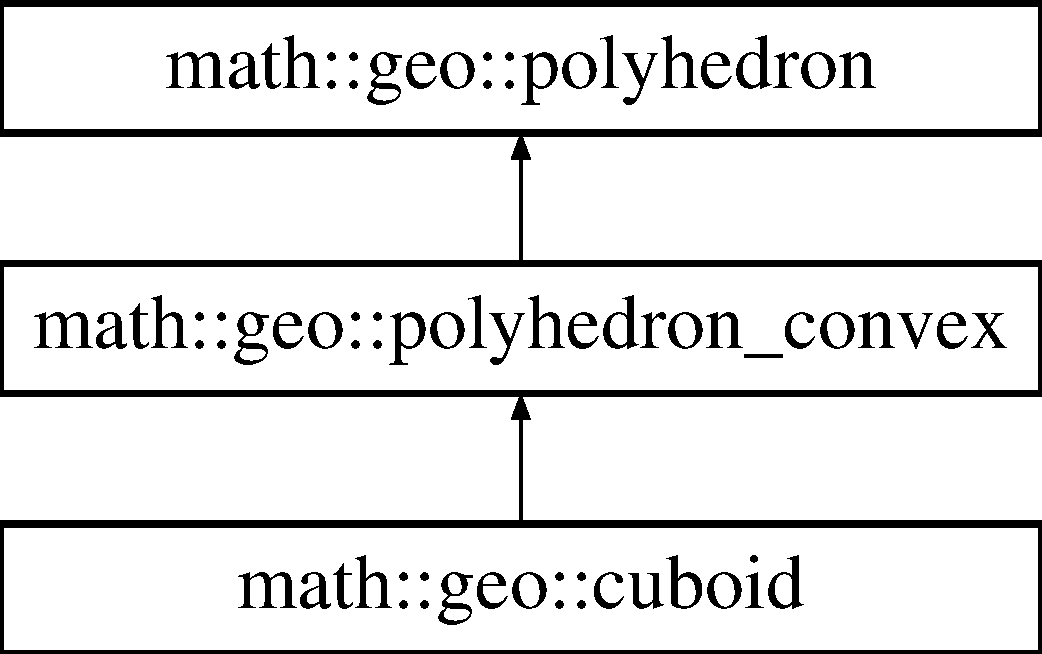
\includegraphics[height=3cm]{classmath_1_1geo_1_1cuboid}
\end{center}
\end{figure}
\subsection*{Public Member Functions}
\begin{DoxyCompactItemize}
\item 
\hypertarget{classmath_1_1geo_1_1cuboid_a72bd7e6bf32ccd6928e375efa3036491}{
{\bfseries cuboid} (float, float, float)}
\label{classmath_1_1geo_1_1cuboid_a72bd7e6bf32ccd6928e375efa3036491}

\end{DoxyCompactItemize}


The documentation for this class was generated from the following file:\begin{DoxyCompactItemize}
\item 
src/math/geo/polyhedron.h\end{DoxyCompactItemize}

\hypertarget{classmath_1_1except_1_1domain}{
\section{math::except::domain Class Reference}
\label{classmath_1_1except_1_1domain}\index{math::except::domain@{math::except::domain}}
}
\subsection*{Public Member Functions}
\begin{DoxyCompactItemize}
\item 
\hypertarget{classmath_1_1except_1_1domain_adb97a428e44d728735fdf1e8c203dd1b}{
const char $\ast$ {\bfseries what} () const   throw ()}
\label{classmath_1_1except_1_1domain_adb97a428e44d728735fdf1e8c203dd1b}

\end{DoxyCompactItemize}


The documentation for this class was generated from the following file:\begin{DoxyCompactItemize}
\item 
src/math/except.hpp\end{DoxyCompactItemize}

\hypertarget{classmath_1_1discrete_1_1Graph_1_1Edge}{
\section{math::discrete::Graph::Edge Class Reference}
\label{classmath_1_1discrete_1_1Graph_1_1Edge}\index{math::discrete::Graph::Edge@{math::discrete::Graph::Edge}}
}
Inheritance diagram for math::discrete::Graph::Edge::\begin{figure}[H]
\begin{center}
\leavevmode
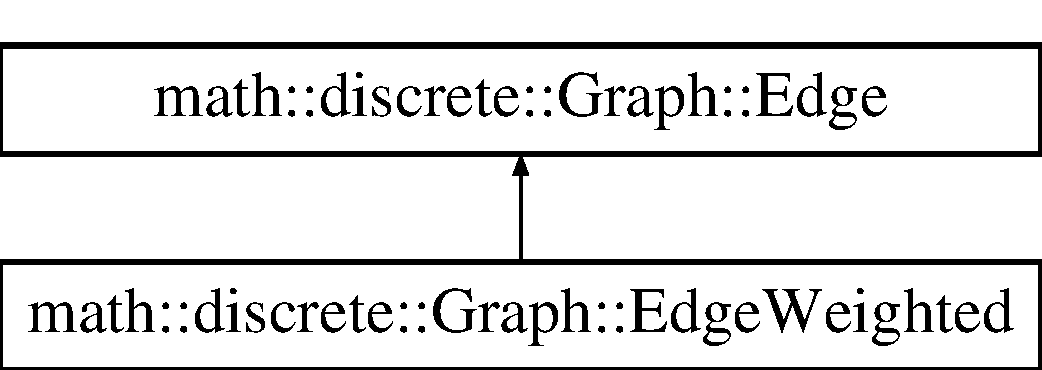
\includegraphics[height=2cm]{classmath_1_1discrete_1_1Graph_1_1Edge}
\end{center}
\end{figure}
\subsection*{Public Attributes}
\begin{DoxyCompactItemize}
\item 
\hypertarget{classmath_1_1discrete_1_1Graph_1_1Edge_a94989ea7055849b7a9e85f33f271ff84}{
\hyperlink{classmath_1_1discrete_1_1Graph_1_1Node}{Node} $\ast$ {\bfseries a\_\-}}
\label{classmath_1_1discrete_1_1Graph_1_1Edge_a94989ea7055849b7a9e85f33f271ff84}

\item 
\hypertarget{classmath_1_1discrete_1_1Graph_1_1Edge_aefa7104cfdbcd7c0e4bb66fd68c4634c}{
\hyperlink{classmath_1_1discrete_1_1Graph_1_1Node}{Node} $\ast$ {\bfseries b\_\-}}
\label{classmath_1_1discrete_1_1Graph_1_1Edge_aefa7104cfdbcd7c0e4bb66fd68c4634c}

\end{DoxyCompactItemize}


The documentation for this class was generated from the following file:\begin{DoxyCompactItemize}
\item 
src/math/discrete/discrete.hpp\end{DoxyCompactItemize}

\hypertarget{classedge}{
\section{edge Class Reference}
\label{classedge}\index{edge@{edge}}
}
Inheritance diagram for edge::\begin{figure}[H]
\begin{center}
\leavevmode
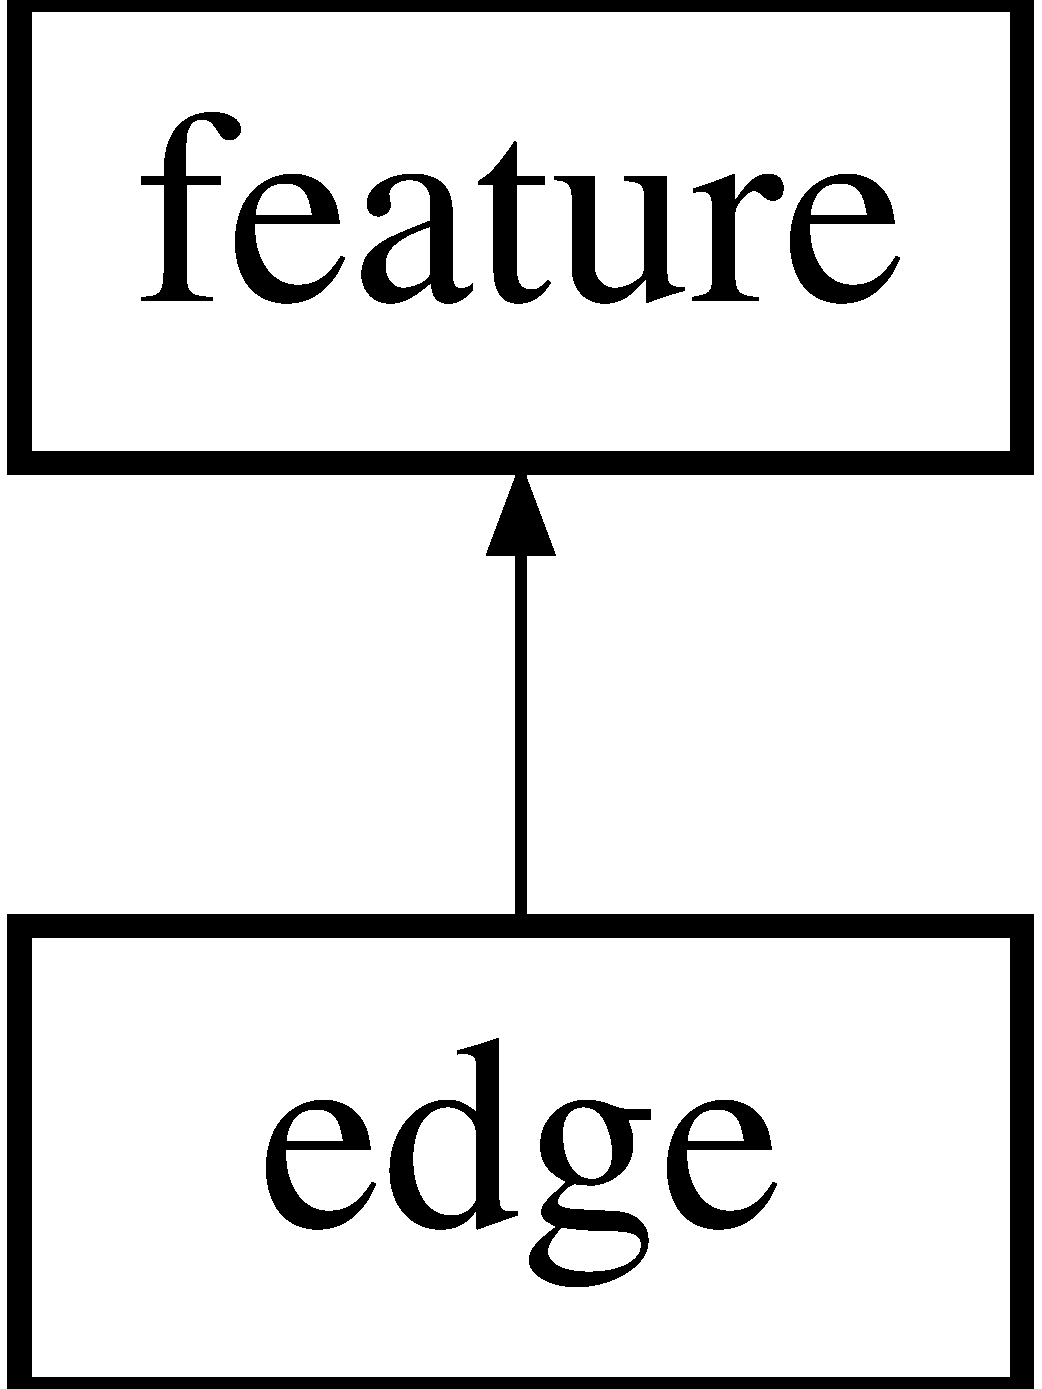
\includegraphics[height=2cm]{classedge}
\end{center}
\end{figure}
\subsection*{Public Member Functions}
\begin{DoxyCompactItemize}
\item 
\hypertarget{classedge_accdb9854acefe81b1dee217abb4c5c55}{
\hyperlink{classmath_1_1vec3}{math::vec3} {\bfseries at} (float l)}
\label{classedge_accdb9854acefe81b1dee217abb4c5c55}

\item 
\hypertarget{classedge_a0fea19012bb1bb4a15e3412977e5d161}{
\hyperlink{classvertex}{vertex} $\ast$ {\bfseries other} (\hyperlink{classvertex}{vertex} $\ast$)}
\label{classedge_a0fea19012bb1bb4a15e3412977e5d161}

\end{DoxyCompactItemize}
\subsection*{Public Attributes}
\begin{DoxyCompactItemize}
\item 
\hypertarget{classedge_ad56afec0fd1621fcc56f24f1edefca19}{
\hyperlink{classmath_1_1vec3}{math::vec3} {\bfseries u}}
\label{classedge_ad56afec0fd1621fcc56f24f1edefca19}

\item 
\hypertarget{classedge_a6c0eb36b7ec40943fcd633c3eda2a206}{
\hyperlink{classvertex}{vertex} $\ast$ {\bfseries t}}
\label{classedge_a6c0eb36b7ec40943fcd633c3eda2a206}

\item 
\hypertarget{classedge_aab93143962ff82c557e7796151d4809f}{
\hyperlink{classvertex}{vertex} $\ast$ {\bfseries h}}
\label{classedge_aab93143962ff82c557e7796151d4809f}

\item 
\hypertarget{classedge_a32f90bcc15f534bc1bd03a535274bacc}{
\hyperlink{classface}{face} $\ast$ {\bfseries f} \mbox{[}2\mbox{]}}
\label{classedge_a32f90bcc15f534bc1bd03a535274bacc}

\end{DoxyCompactItemize}


The documentation for this class was generated from the following file:\begin{DoxyCompactItemize}
\item 
src/math/vclip/vclip.h\end{DoxyCompactItemize}

\hypertarget{classmath_1_1discrete_1_1Graph_1_1EdgeWeighted}{
\section{math::discrete::Graph::EdgeWeighted Class Reference}
\label{classmath_1_1discrete_1_1Graph_1_1EdgeWeighted}\index{math::discrete::Graph::EdgeWeighted@{math::discrete::Graph::EdgeWeighted}}
}
Inheritance diagram for math::discrete::Graph::EdgeWeighted::\begin{figure}[H]
\begin{center}
\leavevmode
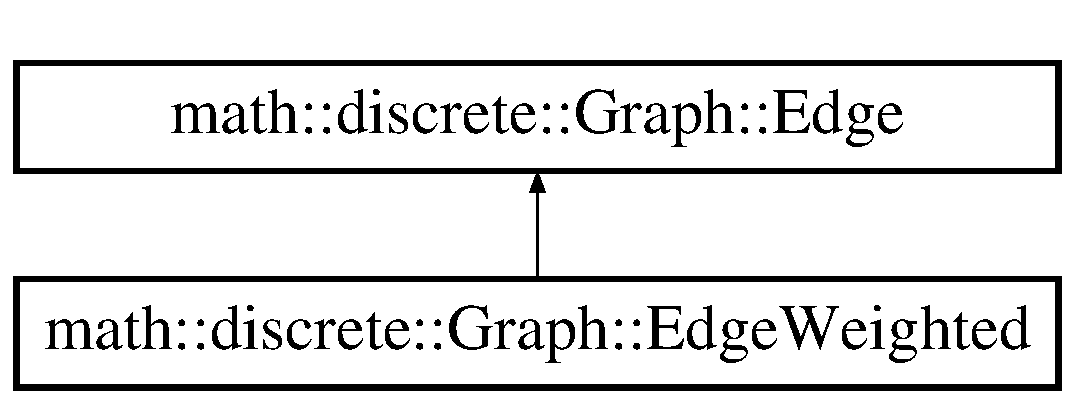
\includegraphics[height=2cm]{classmath_1_1discrete_1_1Graph_1_1EdgeWeighted}
\end{center}
\end{figure}
\subsection*{Public Attributes}
\begin{DoxyCompactItemize}
\item 
\hypertarget{classmath_1_1discrete_1_1Graph_1_1EdgeWeighted_a868b0a21112736710da5e1f1ad16fed3}{
double {\bfseries w\_\-}}
\label{classmath_1_1discrete_1_1Graph_1_1EdgeWeighted_a868b0a21112736710da5e1f1ad16fed3}

\end{DoxyCompactItemize}


The documentation for this class was generated from the following file:\begin{DoxyCompactItemize}
\item 
src/math/discrete/discrete.hpp\end{DoxyCompactItemize}

\hypertarget{classface}{
\section{face Class Reference}
\label{classface}\index{face@{face}}
}
Inheritance diagram for face::\begin{figure}[H]
\begin{center}
\leavevmode
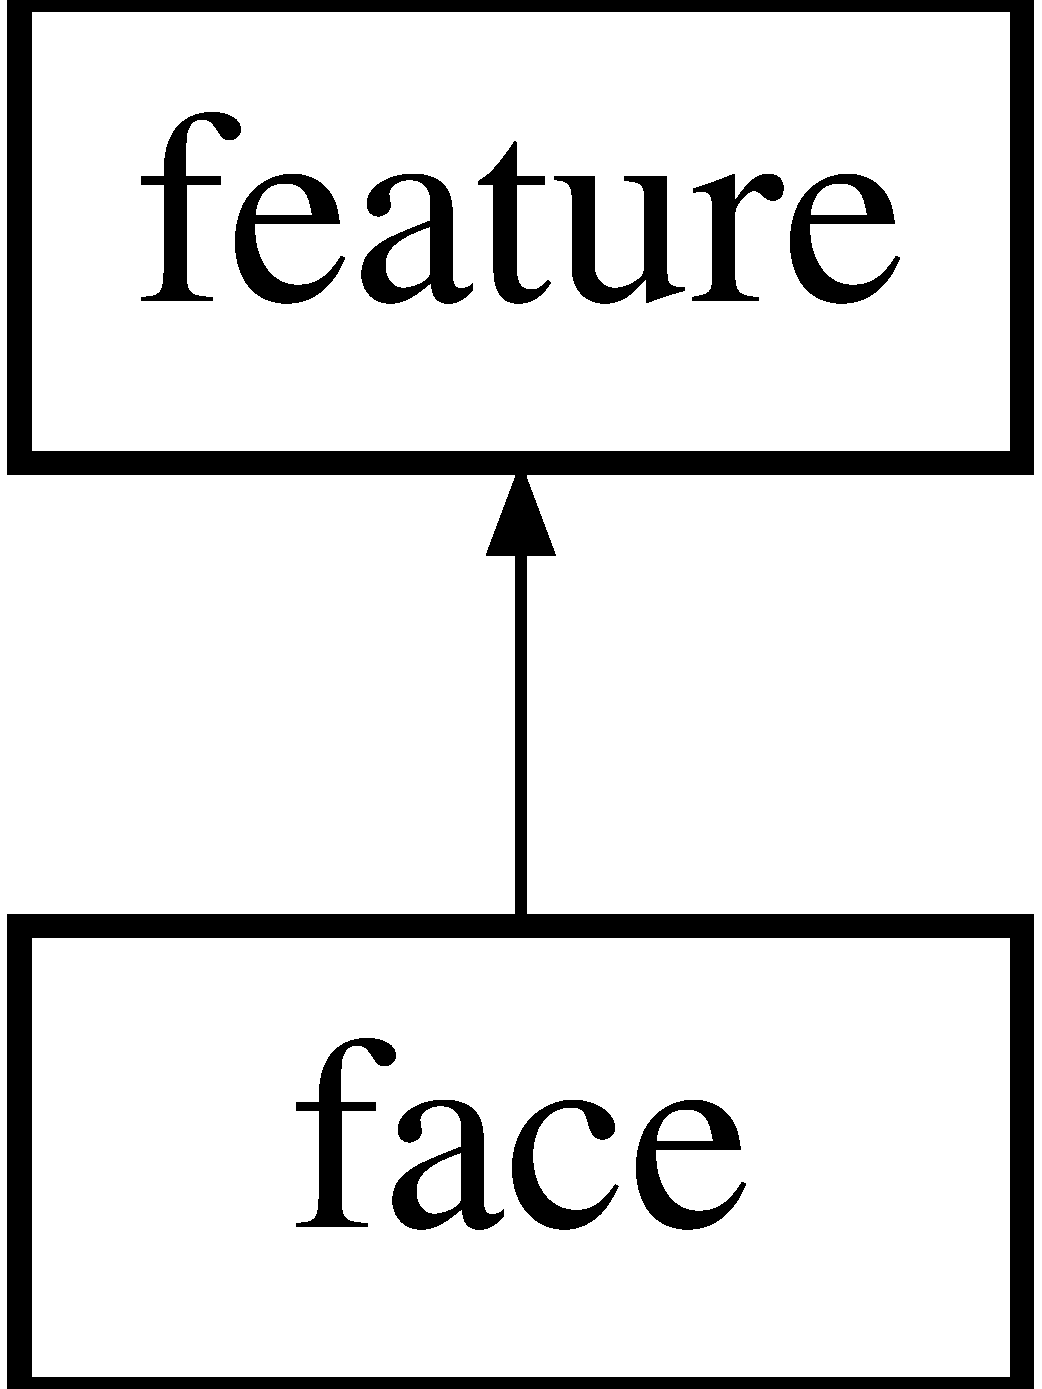
\includegraphics[height=2cm]{classface}
\end{center}
\end{figure}
\subsection*{Public Attributes}
\begin{DoxyCompactItemize}
\item 
\hypertarget{classface_a11e8c57124ede77de5842c52e10472c8}{
std::set$<$ \hyperlink{classfeature}{feature} $\ast$ $>$ {\bfseries e}}
\label{classface_a11e8c57124ede77de5842c52e10472c8}

\item 
\hypertarget{classface_ae494cf85c810c1014bf424e7a39eeaee}{
\hyperlink{classplane}{plane} {\bfseries p}}
\label{classface_ae494cf85c810c1014bf424e7a39eeaee}

\end{DoxyCompactItemize}


The documentation for this class was generated from the following file:\begin{DoxyCompactItemize}
\item 
src/math/vclip/vclip.hpp\end{DoxyCompactItemize}

\hypertarget{classfeature}{
\section{feature Class Reference}
\label{classfeature}\index{feature@{feature}}
}
Inheritance diagram for feature::\begin{figure}[H]
\begin{center}
\leavevmode
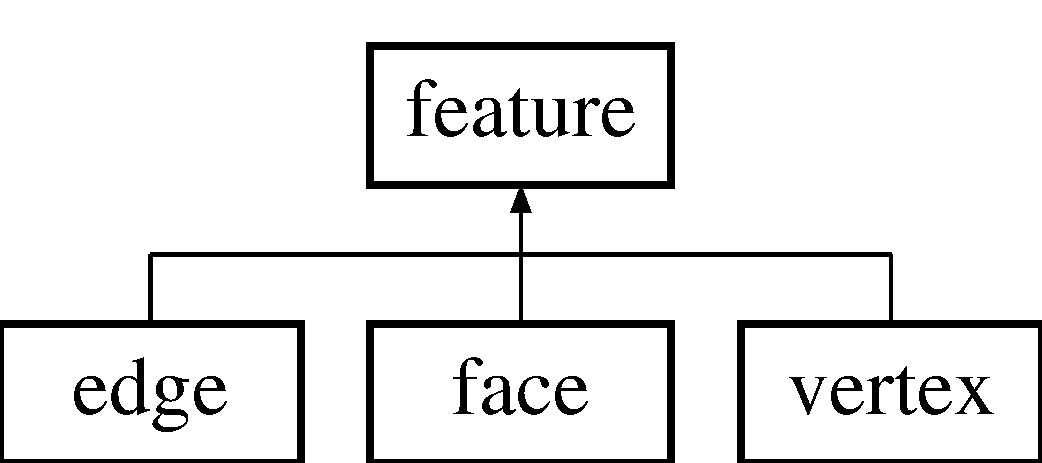
\includegraphics[height=2cm]{classfeature}
\end{center}
\end{figure}


The documentation for this class was generated from the following file:\begin{DoxyCompactItemize}
\item 
src/math/vclip/vclip.hpp\end{DoxyCompactItemize}

\hypertarget{classmath_1_1discrete_1_1Graph_1_1Graph}{
\section{math::discrete::Graph::Graph Class Reference}
\label{classmath_1_1discrete_1_1Graph_1_1Graph}\index{math::discrete::Graph::Graph@{math::discrete::Graph::Graph}}
}
\subsection*{Public Attributes}
\begin{DoxyCompactItemize}
\item 
\hypertarget{classmath_1_1discrete_1_1Graph_1_1Graph_a0a9fb8fc2e45aaa8b910a5b938bfbb9d}{
std::vector$<$ \hyperlink{classmath_1_1discrete_1_1Graph_1_1Node}{Node} $\ast$ $>$ {\bfseries nodes\_\-}}
\label{classmath_1_1discrete_1_1Graph_1_1Graph_a0a9fb8fc2e45aaa8b910a5b938bfbb9d}

\item 
\hypertarget{classmath_1_1discrete_1_1Graph_1_1Graph_aebb0a04782bc28e84f975acdb5d82b41}{
std::vector$<$ \hyperlink{classmath_1_1discrete_1_1Graph_1_1Edge}{Edge} $\ast$ $>$ {\bfseries edges\_\-}}
\label{classmath_1_1discrete_1_1Graph_1_1Graph_aebb0a04782bc28e84f975acdb5d82b41}

\end{DoxyCompactItemize}


The documentation for this class was generated from the following file:\begin{DoxyCompactItemize}
\item 
src/math/discrete/discrete.hpp\end{DoxyCompactItemize}

\hypertarget{classmath_1_1geo_1_1height__map}{
\section{math::geo::height\_\-map Class Reference}
\label{classmath_1_1geo_1_1height__map}\index{math::geo::height\_\-map@{math::geo::height\_\-map}}
}
\subsection*{Public Member Functions}
\begin{DoxyCompactItemize}
\item 
\hypertarget{classmath_1_1geo_1_1height__map_a56685f77f9750167f419366039118113}{
{\bfseries height\_\-map} (int, int)}
\label{classmath_1_1geo_1_1height__map_a56685f77f9750167f419366039118113}

\end{DoxyCompactItemize}
\subsection*{Public Attributes}
\begin{DoxyCompactItemize}
\item 
\hypertarget{classmath_1_1geo_1_1height__map_add2b5f09f8bf6a3d7c674afd0fcb0ee4}{
\hyperlink{classmath_1_1geo_1_1vertex}{vertex} $\ast$ {\bfseries vertices\_\-}}
\label{classmath_1_1geo_1_1height__map_add2b5f09f8bf6a3d7c674afd0fcb0ee4}

\item 
\hypertarget{classmath_1_1geo_1_1height__map_a29abf1041ebd17777d88a2b55ef82535}{
\hyperlink{classmath_1_1geo_1_1tri}{tri} $\ast$ {\bfseries tris\_\-}}
\label{classmath_1_1geo_1_1height__map_a29abf1041ebd17777d88a2b55ef82535}

\end{DoxyCompactItemize}


The documentation for this class was generated from the following files:\begin{DoxyCompactItemize}
\item 
src/math/geo/height\_\-map.hpp\item 
src/math/geo/height\_\-map.cpp\end{DoxyCompactItemize}

\hypertarget{classmath_1_1mat33}{
\section{math::mat33$<$ T $>$ Class Template Reference}
\label{classmath_1_1mat33}\index{math::mat33@{math::mat33}}
}
Inheritance diagram for math::mat33$<$ T $>$::\begin{figure}[H]
\begin{center}
\leavevmode
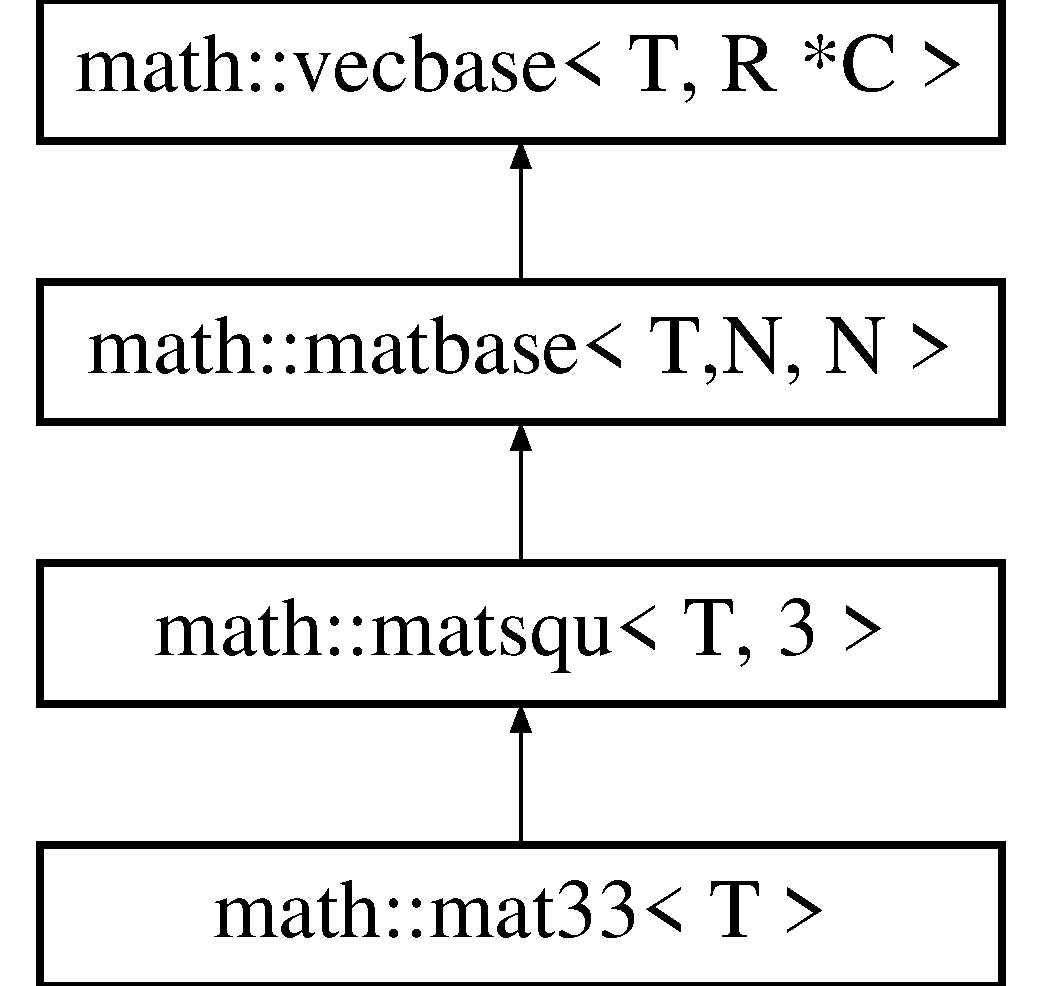
\includegraphics[height=4cm]{classmath_1_1mat33}
\end{center}
\end{figure}
\subsection*{Public Member Functions}
\begin{DoxyCompactItemize}
\item 
\hypertarget{classmath_1_1mat33_ab00020cb1e714e31f4b5d81a02e085d7}{
{\bfseries mat33} (T e0, T e1, T e2, T e3, T e4, T e5, T e6, T e7, T e8)}
\label{classmath_1_1mat33_ab00020cb1e714e31f4b5d81a02e085d7}

\item 
\hypertarget{classmath_1_1mat33_aef2112cfd5ededeeb390a91691a6f469}{
{\bfseries mat33} (\hyperlink{classmath_1_1mat33}{math::mat33}$<$ T $>$ const \&rhs)}
\label{classmath_1_1mat33_aef2112cfd5ededeeb390a91691a6f469}

\item 
\hypertarget{classmath_1_1mat33_ac084f09a588f7c9a1e8874d0b9970339}{
{\bfseries mat33} (const T $\ast$rhs)}
\label{classmath_1_1mat33_ac084f09a588f7c9a1e8874d0b9970339}

\item 
\hypertarget{classmath_1_1mat33_a0603d861a667d254189af5023032854a}{
{\bfseries mat33} (\hyperlink{classmath_1_1vec3}{vec3}$<$ T $>$ const \&rhs)}
\label{classmath_1_1mat33_a0603d861a667d254189af5023032854a}

\item 
\hypertarget{classmath_1_1mat33_a91561f2df87f6cfbac30dcc4b7d44441}{
void {\bfseries setDiagonal} (T x, T y, T z)}
\label{classmath_1_1mat33_a91561f2df87f6cfbac30dcc4b7d44441}

\item 
\hypertarget{classmath_1_1mat33_a66471f4f680e0f9e269e574ee3ff294f}{
void {\bfseries setRotation} (\hyperlink{classmath_1_1quat}{math::quat}$<$ T $>$ const \&q)}
\label{classmath_1_1mat33_a66471f4f680e0f9e269e574ee3ff294f}

\item 
\hypertarget{classmath_1_1mat33_ae141013ac49eba050977b854bfc782bd}{
\hyperlink{classmath_1_1vec3}{math::vec3}$<$ T $>$ {\bfseries getRow} (int position) const }
\label{classmath_1_1mat33_ae141013ac49eba050977b854bfc782bd}

\item 
\hypertarget{classmath_1_1mat33_af742078fad284c80d0ea6366c417ad8c}{
\hyperlink{classmath_1_1vec3}{math::vec3}$<$ T $>$ {\bfseries getColumn} (int position) const }
\label{classmath_1_1mat33_af742078fad284c80d0ea6366c417ad8c}

\item 
\hypertarget{classmath_1_1mat33_a13ec1c970e65b3b77cc1bda61e11e405}{
void {\bfseries loadIdentity} ()}
\label{classmath_1_1mat33_a13ec1c970e65b3b77cc1bda61e11e405}

\item 
\hypertarget{classmath_1_1mat33_ab8e29cb75a9d3a5ac7465701b0d085e7}{
\hyperlink{classmath_1_1mat33}{math::mat33}$<$ T $>$ {\bfseries operator+} (\hyperlink{classmath_1_1mat33}{math::mat33}$<$ T $>$ const \&rhs) const }
\label{classmath_1_1mat33_ab8e29cb75a9d3a5ac7465701b0d085e7}

\item 
\hypertarget{classmath_1_1mat33_a7ff7982969708087c4e9d742ed4b82a9}{
\hyperlink{classmath_1_1mat33}{math::mat33}$<$ T $>$ {\bfseries operator-\/} (\hyperlink{classmath_1_1mat33}{math::mat33}$<$ T $>$ const \&rhs) const }
\label{classmath_1_1mat33_a7ff7982969708087c4e9d742ed4b82a9}

\item 
\hypertarget{classmath_1_1mat33_a539a075bdab7142f1287ad913fb51df6}{
\hyperlink{classmath_1_1mat33}{math::mat33}$<$ T $>$ {\bfseries operator$\ast$} (\hyperlink{classmath_1_1mat33}{math::mat33}$<$ T $>$ const \&rhs) const }
\label{classmath_1_1mat33_a539a075bdab7142f1287ad913fb51df6}

\item 
\hypertarget{classmath_1_1mat33_aa27d6f8275975ebe240ffc3d673170ea}{
\hyperlink{classmath_1_1mat33}{math::mat33}$<$ T $>$ {\bfseries operator$\ast$} (T const \&rhs) const }
\label{classmath_1_1mat33_aa27d6f8275975ebe240ffc3d673170ea}

\item 
\hypertarget{classmath_1_1mat33_aa01273af4a19fc9b1b8ab062c776b64a}{
\hyperlink{classmath_1_1mat33}{math::mat33}$<$ T $>$ {\bfseries operator/} (T const \&rhs) const }
\label{classmath_1_1mat33_aa01273af4a19fc9b1b8ab062c776b64a}

\item 
\hypertarget{classmath_1_1mat33_a85cd630c71cdad7cedaa76ed5bb833d5}{
bool {\bfseries operator==} (\hyperlink{classmath_1_1mat33}{math::mat33}$<$ T $>$ const \&rhs) const }
\label{classmath_1_1mat33_a85cd630c71cdad7cedaa76ed5bb833d5}

\item 
\hypertarget{classmath_1_1mat33_a771bf672147d8f7302cce640d741707c}{
bool {\bfseries operator!=} (const \hyperlink{classmath_1_1mat33}{math::mat33}$<$ T $>$ \&rhs) const }
\label{classmath_1_1mat33_a771bf672147d8f7302cce640d741707c}

\item 
\hypertarget{classmath_1_1mat33_a3cbf3b0094900d864ece681203dc2fa5}{
void {\bfseries operator+=} (const \hyperlink{classmath_1_1mat33}{math::mat33}$<$ T $>$ \&rhs)}
\label{classmath_1_1mat33_a3cbf3b0094900d864ece681203dc2fa5}

\item 
\hypertarget{classmath_1_1mat33_a6b29d96ee8269f39ff96b425940531cd}{
void {\bfseries operator-\/=} (const \hyperlink{classmath_1_1mat33}{math::mat33}$<$ T $>$ \&rhs)}
\label{classmath_1_1mat33_a6b29d96ee8269f39ff96b425940531cd}

\item 
\hypertarget{classmath_1_1mat33_a3aab4bd5fa08664ba84f231684493c36}{
void {\bfseries operator$\ast$=} (const \hyperlink{classmath_1_1mat33}{math::mat33}$<$ T $>$ \&rhs)}
\label{classmath_1_1mat33_a3aab4bd5fa08664ba84f231684493c36}

\item 
\hypertarget{classmath_1_1mat33_a31a1e0240ed69565f6806484bc299de5}{
\hyperlink{classmath_1_1vec3}{math::vec3}$<$ T $>$ {\bfseries operator$\ast$} (const \hyperlink{classmath_1_1vec3}{vec3}$<$ T $>$ rhs) const }
\label{classmath_1_1mat33_a31a1e0240ed69565f6806484bc299de5}

\item 
\hypertarget{classmath_1_1mat33_abb59ea70e98766225e62a8387bb226b2}{
\hyperlink{classmath_1_1vec3}{math::vec3}$<$ T $>$ {\bfseries getRotatedVector3D} (const \hyperlink{classmath_1_1vec3}{vec3}$<$ T $>$ \&rhs) const }
\label{classmath_1_1mat33_abb59ea70e98766225e62a8387bb226b2}

\item 
\hypertarget{classmath_1_1mat33_aeb611d48183298eae28cf4f7bba747df}{
\hyperlink{classmath_1_1vec3}{math::vec3}$<$ T $>$ {\bfseries getInverseRotatedVector3D} (const \hyperlink{classmath_1_1vec3}{vec3}$<$ T $>$ \&rhs) const }
\label{classmath_1_1mat33_aeb611d48183298eae28cf4f7bba747df}

\item 
\hypertarget{classmath_1_1mat33_a4669d8706bdfcd57647c98d6ba52128b}{
void {\bfseries invert} ()}
\label{classmath_1_1mat33_a4669d8706bdfcd57647c98d6ba52128b}

\item 
\hypertarget{classmath_1_1mat33_aec8b7fb7359e71e6b75cb2d0f26f17b3}{
\hyperlink{classmath_1_1mat33}{math::mat33}$<$ T $>$ {\bfseries getInverse} () const }
\label{classmath_1_1mat33_aec8b7fb7359e71e6b75cb2d0f26f17b3}

\item 
\hypertarget{classmath_1_1mat33_aa65877efa975cdfdc28379d819eb2d68}{
void {\bfseries transpose} ()}
\label{classmath_1_1mat33_aa65877efa975cdfdc28379d819eb2d68}

\item 
\hypertarget{classmath_1_1mat33_ac1317114d3719757e234616986c9eecf}{
\hyperlink{classmath_1_1mat33}{math::mat33}$<$ T $>$ {\bfseries getTranspose} (void) const }
\label{classmath_1_1mat33_ac1317114d3719757e234616986c9eecf}

\item 
\hypertarget{classmath_1_1mat33_ae2a0de13e9b6e61892d6d4f5d0db90d6}{
void {\bfseries invertTranspose} (void)}
\label{classmath_1_1mat33_ae2a0de13e9b6e61892d6d4f5d0db90d6}

\item 
\hypertarget{classmath_1_1mat33_a314e156440bf0db6dc26192f0059992a}{
\hyperlink{classmath_1_1mat33}{math::mat33}$<$ T $>$ {\bfseries getInverseTranspose} (void) const }
\label{classmath_1_1mat33_a314e156440bf0db6dc26192f0059992a}

\item 
\hypertarget{classmath_1_1mat33_ac4f9f3ede459490b1c44a35abab4a54f}{
void {\bfseries setRotationAxis} (const T angle, const \hyperlink{classmath_1_1vec3}{vec3}$<$ T $>$ \&axis)}
\label{classmath_1_1mat33_ac4f9f3ede459490b1c44a35abab4a54f}

\item 
\hypertarget{classmath_1_1mat33_ad90a375f88206f2aa1571703a5b2adc8}{
void {\bfseries setRotationX} (const T angle)}
\label{classmath_1_1mat33_ad90a375f88206f2aa1571703a5b2adc8}

\item 
\hypertarget{classmath_1_1mat33_aa586fc1b0b2e6c0310a92a181799830d}{
void {\bfseries setRotationY} (const T angle)}
\label{classmath_1_1mat33_aa586fc1b0b2e6c0310a92a181799830d}

\item 
\hypertarget{classmath_1_1mat33_a41c805f2e577826071e5cb95ebe6b8c7}{
void {\bfseries setRotationZ} (const T angle)}
\label{classmath_1_1mat33_a41c805f2e577826071e5cb95ebe6b8c7}

\item 
\hypertarget{classmath_1_1mat33_aee554b3afc31de39404cede72b659e75}{
void {\bfseries setRotationEuler} (const T angleX, const T angleY, const T angleZ)}
\label{classmath_1_1mat33_aee554b3afc31de39404cede72b659e75}

\item 
\hypertarget{classmath_1_1mat33_af4e344f4a07bc0eb5c003cef663e9cc2}{
void {\bfseries rotateVector3D} (\hyperlink{classmath_1_1vec3}{math::vec3}$<$ T $>$ \&rhs) const }
\label{classmath_1_1mat33_af4e344f4a07bc0eb5c003cef663e9cc2}

\item 
\hypertarget{classmath_1_1mat33_aaa5aa7bf812c1edf162c90a937f77d92}{
void {\bfseries inverseRotateVector3D} (\hyperlink{classmath_1_1vec3}{math::vec3}$<$ T $>$ \&rhs) const }
\label{classmath_1_1mat33_aaa5aa7bf812c1edf162c90a937f77d92}

\item 
\hypertarget{classmath_1_1mat33_ad1b3ef329d70bffaae957a7e871ea29a}{
{\bfseries operator T $\ast$} () const }
\label{classmath_1_1mat33_ad1b3ef329d70bffaae957a7e871ea29a}

\item 
\hypertarget{classmath_1_1mat33_a727616b6c5fa235e4e48b61e41996fb1}{
{\bfseries operator const T $\ast$} () const }
\label{classmath_1_1mat33_a727616b6c5fa235e4e48b61e41996fb1}

\end{DoxyCompactItemize}
\subsubsection*{template$<$typename T$>$ class math::mat33$<$ T $>$}



The documentation for this class was generated from the following file:\begin{DoxyCompactItemize}
\item 
src/math/mat33.hpp\end{DoxyCompactItemize}

\hypertarget{classmath_1_1mat44}{
\section{math::mat44$<$ T $>$ Class Template Reference}
\label{classmath_1_1mat44}\index{math::mat44@{math::mat44}}
}
Inheritance diagram for math::mat44$<$ T $>$::\begin{figure}[H]
\begin{center}
\leavevmode
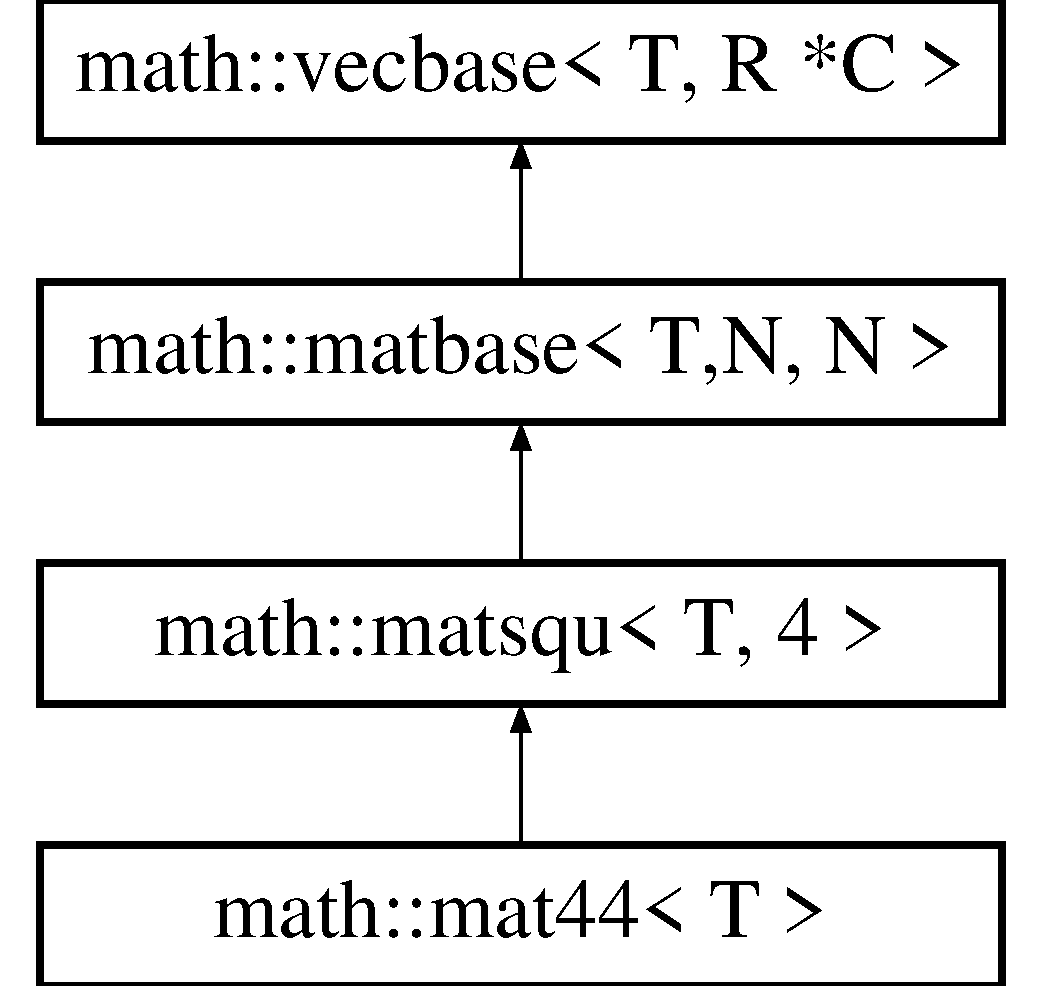
\includegraphics[height=4cm]{classmath_1_1mat44}
\end{center}
\end{figure}
\subsection*{Public Member Functions}
\begin{DoxyCompactItemize}
\item 
\hypertarget{classmath_1_1mat44_a1130dbd465b9d6d47fb5ee2f12ed23f0}{
{\bfseries mat44} (T, T, T, T, T, T, T, T, T, T, T, T, T, T, T, T)}
\label{classmath_1_1mat44_a1130dbd465b9d6d47fb5ee2f12ed23f0}

\item 
\hypertarget{classmath_1_1mat44_ad21b555ef817572be46000ece4b87a1a}{
{\bfseries mat44} (const T $\ast$rhs)}
\label{classmath_1_1mat44_ad21b555ef817572be46000ece4b87a1a}

\item 
\hypertarget{classmath_1_1mat44_a9d291f8d0a8f45914266395a59747c6b}{
{\bfseries mat44} (const \hyperlink{classmath_1_1mat44}{mat44} \&rhs)}
\label{classmath_1_1mat44_a9d291f8d0a8f45914266395a59747c6b}

\item 
\hypertarget{classmath_1_1mat44_a0214f4c0946a0c322a3873348ba260ba}{
{\bfseries mat44} (\hyperlink{classmath_1_1quat}{quat}$<$ T $>$ const \&q)}
\label{classmath_1_1mat44_a0214f4c0946a0c322a3873348ba260ba}

\item 
\hypertarget{classmath_1_1mat44_a33f5451d462044844a2e581541fa80c0}{
{\bfseries mat44} (\hyperlink{classmath_1_1transform}{transform}$<$ T $>$ const \&)}
\label{classmath_1_1mat44_a33f5451d462044844a2e581541fa80c0}

\item 
\hypertarget{classmath_1_1mat44_a2ccdbfc7e205429f50c98babcb1187d8}{
void {\bfseries SetEntry} (int position, T value)}
\label{classmath_1_1mat44_a2ccdbfc7e205429f50c98babcb1187d8}

\item 
\hypertarget{classmath_1_1mat44_a9533b8b54e9a0d7fed4a63645348f84b}{
T {\bfseries GetEntry} (int position) const }
\label{classmath_1_1mat44_a9533b8b54e9a0d7fed4a63645348f84b}

\item 
\hypertarget{classmath_1_1mat44_a604cea86b7b71cd14ad28f534886eec3}{
\hyperlink{classmath_1_1vec4}{vec4}$<$ T $>$ {\bfseries GetRow} (int position) const }
\label{classmath_1_1mat44_a604cea86b7b71cd14ad28f534886eec3}

\item 
\hypertarget{classmath_1_1mat44_aaf0e6b80e5b56bfcdaf4321054935249}{
\hyperlink{classmath_1_1vec4}{vec4}$<$ T $>$ {\bfseries GetColumn} (int position) const }
\label{classmath_1_1mat44_aaf0e6b80e5b56bfcdaf4321054935249}

\item 
\hypertarget{classmath_1_1mat44_a4b24914ce71486394ed4dad05c2c7515}{
void {\bfseries LoadIdentity} (void)}
\label{classmath_1_1mat44_a4b24914ce71486394ed4dad05c2c7515}

\item 
\hypertarget{classmath_1_1mat44_afb3f26027d06fd1879942ddf3ce0f766}{
void {\bfseries LoadZero} (void)}
\label{classmath_1_1mat44_afb3f26027d06fd1879942ddf3ce0f766}

\item 
\hypertarget{classmath_1_1mat44_ad54828d267d7e0d994bbd8e46fa7fd7b}{
\hyperlink{classmath_1_1mat44}{mat44} {\bfseries operator+} (const \hyperlink{classmath_1_1mat44}{mat44} \&rhs) const }
\label{classmath_1_1mat44_ad54828d267d7e0d994bbd8e46fa7fd7b}

\item 
\hypertarget{classmath_1_1mat44_ae31338e54349a6bb9976c7ebdaaf2580}{
\hyperlink{classmath_1_1mat44}{mat44} {\bfseries operator-\/} (const \hyperlink{classmath_1_1mat44}{mat44} \&rhs) const }
\label{classmath_1_1mat44_ae31338e54349a6bb9976c7ebdaaf2580}

\item 
\hypertarget{classmath_1_1mat44_a4ce5cc4349579cac111597f9d7e19b4d}{
\hyperlink{classmath_1_1mat44}{mat44} {\bfseries operator$\ast$} (const \hyperlink{classmath_1_1mat44}{mat44} \&rhs) const }
\label{classmath_1_1mat44_a4ce5cc4349579cac111597f9d7e19b4d}

\item 
\hypertarget{classmath_1_1mat44_a79a39257eda9a0a2dfb5d724b54fa220}{
\hyperlink{classmath_1_1mat44}{mat44} {\bfseries operator$\ast$} (const T rhs) const }
\label{classmath_1_1mat44_a79a39257eda9a0a2dfb5d724b54fa220}

\item 
\hypertarget{classmath_1_1mat44_a9a7c3faf1f878a5d121b2c2cc6388bc9}{
\hyperlink{classmath_1_1mat44}{mat44} {\bfseries operator/} (const T rhs) const }
\label{classmath_1_1mat44_a9a7c3faf1f878a5d121b2c2cc6388bc9}

\item 
\hypertarget{classmath_1_1mat44_a9e7d0e0f7d1c347c9ff4b5a51ec514e7}{
bool {\bfseries operator==} (const \hyperlink{classmath_1_1mat44}{mat44} \&rhs) const }
\label{classmath_1_1mat44_a9e7d0e0f7d1c347c9ff4b5a51ec514e7}

\item 
\hypertarget{classmath_1_1mat44_a35b01d1482c920d54fecee8dea27137e}{
bool {\bfseries operator!=} (const \hyperlink{classmath_1_1mat44}{mat44} \&rhs) const }
\label{classmath_1_1mat44_a35b01d1482c920d54fecee8dea27137e}

\item 
\hypertarget{classmath_1_1mat44_a17307056c74a98b0663904d602b3bb43}{
void {\bfseries operator+=} (const \hyperlink{classmath_1_1mat44}{mat44} \&rhs)}
\label{classmath_1_1mat44_a17307056c74a98b0663904d602b3bb43}

\item 
\hypertarget{classmath_1_1mat44_ad6f05f63f3d4b0c357c954ad6a95473f}{
void {\bfseries operator-\/=} (const \hyperlink{classmath_1_1mat44}{mat44} \&rhs)}
\label{classmath_1_1mat44_ad6f05f63f3d4b0c357c954ad6a95473f}

\item 
\hypertarget{classmath_1_1mat44_ad148a7f58b1ddefe306871bb45b9db24}{
void {\bfseries operator$\ast$=} (const \hyperlink{classmath_1_1mat44}{mat44} \&rhs)}
\label{classmath_1_1mat44_ad148a7f58b1ddefe306871bb45b9db24}

\item 
\hypertarget{classmath_1_1mat44_a94e0057189c9ab80a4210e86b37d2450}{
void {\bfseries operator$\ast$=} (const T rhs)}
\label{classmath_1_1mat44_a94e0057189c9ab80a4210e86b37d2450}

\item 
\hypertarget{classmath_1_1mat44_ad77cac714b0e06705bf46a61527edf4e}{
void {\bfseries operator/=} (const T rhs)}
\label{classmath_1_1mat44_ad77cac714b0e06705bf46a61527edf4e}

\item 
\hypertarget{classmath_1_1mat44_a678c4c500c35a6ac7c9cbfa07544b82f}{
\hyperlink{classmath_1_1mat44}{mat44} {\bfseries operator-\/} (void) const }
\label{classmath_1_1mat44_a678c4c500c35a6ac7c9cbfa07544b82f}

\item 
\hypertarget{classmath_1_1mat44_afaa3ec8ef1b6425899cd054530152b6f}{
\hyperlink{classmath_1_1mat44}{mat44} {\bfseries operator+} (void) const }
\label{classmath_1_1mat44_afaa3ec8ef1b6425899cd054530152b6f}

\item 
\hypertarget{classmath_1_1mat44_a900b2ae1460e40680251cfff5d94b204}{
\hyperlink{classmath_1_1vec4}{vec4}$<$ T $>$ {\bfseries operator$\ast$} (const \hyperlink{classmath_1_1vec4}{vec4}$<$ T $>$ rhs) const }
\label{classmath_1_1mat44_a900b2ae1460e40680251cfff5d94b204}

\item 
\hypertarget{classmath_1_1mat44_ab9a5739e491dea7860248150e052cfc9}{
void {\bfseries RotateVector3D} (\hyperlink{classmath_1_1vec3}{vec3}$<$ double $>$ \&rhs) const }
\label{classmath_1_1mat44_ab9a5739e491dea7860248150e052cfc9}

\item 
\hypertarget{classmath_1_1mat44_a47e1b4c2b8a7402cbe2f810d9ad17e48}{
void {\bfseries InverseRotateVector3D} (\hyperlink{classmath_1_1vec3}{vec3}$<$ double $>$ \&rhs) const }
\label{classmath_1_1mat44_a47e1b4c2b8a7402cbe2f810d9ad17e48}

\item 
\hypertarget{classmath_1_1mat44_aef14aa49d3b4d63a891b7058516e9cb3}{
\hyperlink{classmath_1_1vec3}{vec3}$<$ double $>$ {\bfseries GetRotatedVector3D} (const \hyperlink{classmath_1_1vec3}{vec3}$<$ double $>$ \&rhs) const }
\label{classmath_1_1mat44_aef14aa49d3b4d63a891b7058516e9cb3}

\item 
\hypertarget{classmath_1_1mat44_a5cae23cf2b5f880e955b0a61590e9ccc}{
\hyperlink{classmath_1_1vec3}{vec3}$<$ double $>$ {\bfseries GetInverseRotatedVector3D} (const \hyperlink{classmath_1_1vec3}{vec3}$<$ double $>$ \&rhs) const }
\label{classmath_1_1mat44_a5cae23cf2b5f880e955b0a61590e9ccc}

\item 
\hypertarget{classmath_1_1mat44_ad89781736c0f006bb60be5683e5a707b}{
void {\bfseries TranslateVector3D} (\hyperlink{classmath_1_1vec3}{vec3}$<$ double $>$ \&) const }
\label{classmath_1_1mat44_ad89781736c0f006bb60be5683e5a707b}

\item 
\hypertarget{classmath_1_1mat44_afd776d21e9157bf6d874aa14c0e340b6}{
void {\bfseries InverseTranslateVector3D} (\hyperlink{classmath_1_1vec3}{vec3}$<$ double $>$ \&) const }
\label{classmath_1_1mat44_afd776d21e9157bf6d874aa14c0e340b6}

\item 
\hypertarget{classmath_1_1mat44_a00b596b2c158263d4f5ee44f6bf314ae}{
\hyperlink{classmath_1_1vec3}{vec3}$<$ double $>$ {\bfseries GetTranslatedVector3D} (const \hyperlink{classmath_1_1vec3}{vec3}$<$ double $>$ \&rhs) const }
\label{classmath_1_1mat44_a00b596b2c158263d4f5ee44f6bf314ae}

\item 
\hypertarget{classmath_1_1mat44_a3a507ad33927391da88d2aaa928b15e6}{
\hyperlink{classmath_1_1vec3}{vec3}$<$ double $>$ {\bfseries GetInverseTranslatedVector3D} (const \hyperlink{classmath_1_1vec3}{vec3}$<$ double $>$ \&rhs) const }
\label{classmath_1_1mat44_a3a507ad33927391da88d2aaa928b15e6}

\item 
\hypertarget{classmath_1_1mat44_a0c01cca98e876ad0c8f5c125dfe1feaf}{
void {\bfseries Invert} (void)}
\label{classmath_1_1mat44_a0c01cca98e876ad0c8f5c125dfe1feaf}

\item 
\hypertarget{classmath_1_1mat44_a0feaba4758ed52bac10f26fd799e2de3}{
\hyperlink{classmath_1_1mat44}{mat44} {\bfseries GetInverse} (void) const }
\label{classmath_1_1mat44_a0feaba4758ed52bac10f26fd799e2de3}

\item 
\hypertarget{classmath_1_1mat44_adc6ecd07ee39f9fe10513df7f30155dd}{
void {\bfseries Transpose} (void)}
\label{classmath_1_1mat44_adc6ecd07ee39f9fe10513df7f30155dd}

\item 
\hypertarget{classmath_1_1mat44_aa51cb99def454576932a5162256d517a}{
\hyperlink{classmath_1_1mat44}{mat44} {\bfseries GetTranspose} (void) const }
\label{classmath_1_1mat44_aa51cb99def454576932a5162256d517a}

\item 
\hypertarget{classmath_1_1mat44_a6460a465e3d8ae718f1e5abe95c9e25c}{
void {\bfseries InvertTranspose} (void)}
\label{classmath_1_1mat44_a6460a465e3d8ae718f1e5abe95c9e25c}

\item 
\hypertarget{classmath_1_1mat44_aa022f83245b05ffe83bf8e4ee5138f00}{
\hyperlink{classmath_1_1mat44}{mat44} {\bfseries GetInverseTranspose} (void) const }
\label{classmath_1_1mat44_aa022f83245b05ffe83bf8e4ee5138f00}

\item 
\hypertarget{classmath_1_1mat44_a3fb20ac063bbc5921bcaeb3ac92ab35b}{
void {\bfseries SetCoordinateTransform} (\hyperlink{classmath_1_1vec3}{math::vec3}$<$ double $>$ const, \hyperlink{classmath_1_1vec3}{math::vec3}$<$ double $>$ const)}
\label{classmath_1_1mat44_a3fb20ac063bbc5921bcaeb3ac92ab35b}

\item 
\hypertarget{classmath_1_1mat44_a7c09a54e77d1277e1f341d0a0ab88011}{
void {\bfseries AffineInvert} (void)}
\label{classmath_1_1mat44_a7c09a54e77d1277e1f341d0a0ab88011}

\item 
\hypertarget{classmath_1_1mat44_a5bb524e4b19475c5a36bad44689b557a}{
\hyperlink{classmath_1_1mat44}{mat44} {\bfseries GetAffineInverse} (void) const }
\label{classmath_1_1mat44_a5bb524e4b19475c5a36bad44689b557a}

\item 
\hypertarget{classmath_1_1mat44_aee84b07ad0b747d0aef09a975713f3a3}{
void {\bfseries AffineInvertTranspose} (void)}
\label{classmath_1_1mat44_aee84b07ad0b747d0aef09a975713f3a3}

\item 
\hypertarget{classmath_1_1mat44_a5a619a1605d048b1e01d904cd0dc31d7}{
\hyperlink{classmath_1_1mat44}{mat44} {\bfseries GetAffineInverseTranspose} (void) const }
\label{classmath_1_1mat44_a5a619a1605d048b1e01d904cd0dc31d7}

\item 
\hypertarget{classmath_1_1mat44_a47696d5728bb8a42d4e38923b3be9708}{
void {\bfseries SetTranslation} (\hyperlink{classmath_1_1vec3}{vec3}$<$ double $>$ const \&)}
\label{classmath_1_1mat44_a47696d5728bb8a42d4e38923b3be9708}

\item 
\hypertarget{classmath_1_1mat44_a311b3320b1cbaaeb2189b2db1883fec7}{
void {\bfseries SetScale} (\hyperlink{classmath_1_1vec3}{vec3}$<$ double $>$ const \&)}
\label{classmath_1_1mat44_a311b3320b1cbaaeb2189b2db1883fec7}

\item 
\hypertarget{classmath_1_1mat44_a6a0d5ddb6df2dc6568f0d6a95f302d3b}{
void {\bfseries SetUniformScale} (const T scaleFactor)}
\label{classmath_1_1mat44_a6a0d5ddb6df2dc6568f0d6a95f302d3b}

\item 
\hypertarget{classmath_1_1mat44_a7f7ea68fd2c7b30804204cc70d713d52}{
void {\bfseries set\_\-rotation} (\hyperlink{classmath_1_1quat}{quat}$<$ T $>$ const \&)}
\label{classmath_1_1mat44_a7f7ea68fd2c7b30804204cc70d713d52}

\item 
\hypertarget{classmath_1_1mat44_a157b37473ff94c7487d69d0f72c14f5a}{
void {\bfseries SetRotationAxis} (const double angle, const \hyperlink{classmath_1_1vec3}{vec3}$<$ double $>$ \&axis)}
\label{classmath_1_1mat44_a157b37473ff94c7487d69d0f72c14f5a}

\item 
\hypertarget{classmath_1_1mat44_a8a3e080f62685e9df01d1fb07249d11d}{
void {\bfseries SetRotationX} (const T angle)}
\label{classmath_1_1mat44_a8a3e080f62685e9df01d1fb07249d11d}

\item 
\hypertarget{classmath_1_1mat44_a55e437444524b0a3d2273ca5987d59be}{
void {\bfseries SetRotationY} (const T angle)}
\label{classmath_1_1mat44_a55e437444524b0a3d2273ca5987d59be}

\item 
\hypertarget{classmath_1_1mat44_a5707e8c3e1f52ba05809b210103bbe8a}{
void {\bfseries SetRotationZ} (const T angle)}
\label{classmath_1_1mat44_a5707e8c3e1f52ba05809b210103bbe8a}

\item 
\hypertarget{classmath_1_1mat44_a7885a6c4037a8dc93e2f630bf419ac9a}{
void {\bfseries SetRotationEuler} (const double angleX, const double, const double angleZ)}
\label{classmath_1_1mat44_a7885a6c4037a8dc93e2f630bf419ac9a}

\item 
\hypertarget{classmath_1_1mat44_a9294493b17f600d38346d6d683ddd918}{
void {\bfseries SetPerspective} (T, T, T, T, T, T)}
\label{classmath_1_1mat44_a9294493b17f600d38346d6d683ddd918}

\item 
\hypertarget{classmath_1_1mat44_afd9ae3ec67c631724edca366a6b518cf}{
void {\bfseries SetPerspective} (T fovy, T aspect, T n, T f)}
\label{classmath_1_1mat44_afd9ae3ec67c631724edca366a6b518cf}

\item 
\hypertarget{classmath_1_1mat44_a6978c6c7b4303eb2defcbaecf24892b3}{
void {\bfseries SetOrtho} (T left, T right, T bottom, T top, T n, T f)}
\label{classmath_1_1mat44_a6978c6c7b4303eb2defcbaecf24892b3}

\item 
\hypertarget{classmath_1_1mat44_a8a983b0ba8e01e1a5461ef53fe4d98c6}{
void {\bfseries setLookAt} (\hyperlink{classmath_1_1vec3}{math::vec3}$<$ double $>$ eye, \hyperlink{classmath_1_1vec3}{math::vec3}$<$ double $>$ center, \hyperlink{classmath_1_1vec3}{math::vec3}$<$ double $>$ up)}
\label{classmath_1_1mat44_a8a983b0ba8e01e1a5461ef53fe4d98c6}

\item 
\hypertarget{classmath_1_1mat44_adac3ed3f879878f367e9d49e3ab16e05}{
void {\bfseries SetReflection} (\hyperlink{classmath_1_1plane}{plane}$<$ T $>$ const \&)}
\label{classmath_1_1mat44_adac3ed3f879878f367e9d49e3ab16e05}

\item 
\hypertarget{classmath_1_1mat44_abde01621efccb6954077023e33b4f1c0}{
void {\bfseries print} ()}
\label{classmath_1_1mat44_abde01621efccb6954077023e33b4f1c0}

\item 
\hypertarget{classmath_1_1mat44_adfefea95fc901a16a54def48636aa52d}{
void {\bfseries SetTranslationPart} (\hyperlink{classmath_1_1vec3}{vec3}$<$ double $>$ const \&)}
\label{classmath_1_1mat44_adfefea95fc901a16a54def48636aa52d}

\item 
\hypertarget{classmath_1_1mat44_a2929e412449d245d485011605bd22b84}{
void {\bfseries SetRotationPartEuler} (double const, double const, double const)}
\label{classmath_1_1mat44_a2929e412449d245d485011605bd22b84}

\item 
\hypertarget{classmath_1_1mat44_a3e2319531f33cb187cdb6a521b2bcd50}{
void {\bfseries SetRotationPartEuler} (\hyperlink{classmath_1_1vec3}{vec3}$<$ double $>$ const \&rotations)}
\label{classmath_1_1mat44_a3e2319531f33cb187cdb6a521b2bcd50}

\item 
\hypertarget{classmath_1_1mat44_a20dcec664e454262299ac5b873002b76}{
{\bfseries operator T $\ast$} () const }
\label{classmath_1_1mat44_a20dcec664e454262299ac5b873002b76}

\item 
\hypertarget{classmath_1_1mat44_a0595a19c2b67bc5e81037ea7490d5d51}{
{\bfseries operator const T $\ast$} () const }
\label{classmath_1_1mat44_a0595a19c2b67bc5e81037ea7490d5d51}

\end{DoxyCompactItemize}
\subsubsection*{template$<$typename T$>$ class math::mat44$<$ T $>$}



The documentation for this class was generated from the following files:\begin{DoxyCompactItemize}
\item 
src/math/mat44.hpp\item 
src/math/mat44.cpp\end{DoxyCompactItemize}

\hypertarget{classmath_1_1matbase}{
\section{math::matbase$<$ T, R, C $>$ Class Template Reference}
\label{classmath_1_1matbase}\index{math::matbase@{math::matbase}}
}
Inheritance diagram for math::matbase$<$ T, R, C $>$::\begin{figure}[H]
\begin{center}
\leavevmode
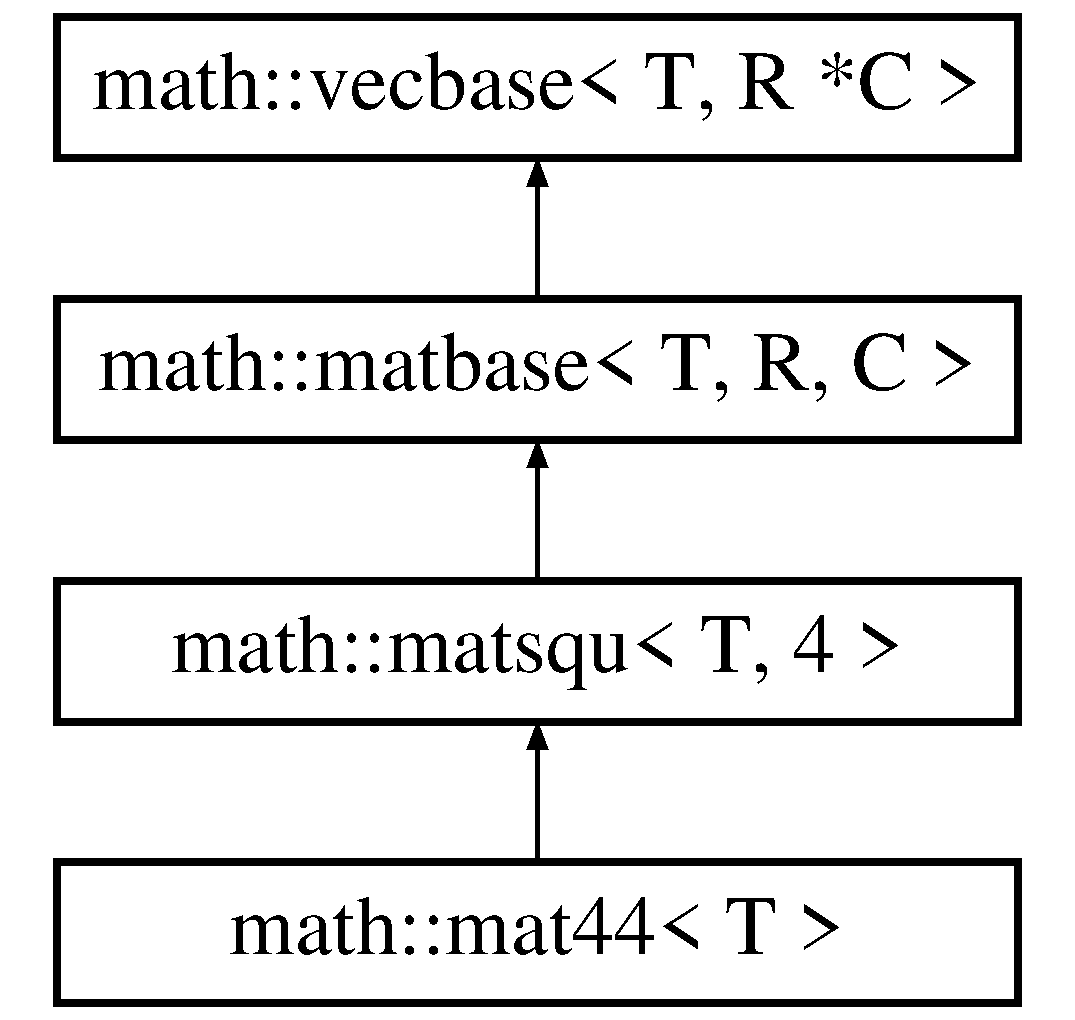
\includegraphics[height=4cm]{classmath_1_1matbase}
\end{center}
\end{figure}
\subsection*{Public Member Functions}
\begin{DoxyCompactItemize}
\item 
\hypertarget{classmath_1_1matbase_ac89f35bb51c718bd42cc7032891708e0}{
{\bfseries matbase} (\hyperlink{classmath_1_1matbase}{math::matbase}$<$ T, R, C $>$ const \&rhs)}
\label{classmath_1_1matbase_ac89f35bb51c718bd42cc7032891708e0}

\item 
\hypertarget{classmath_1_1matbase_af068cbc67739326385ac9eabf8552839}{
{\bfseries matbase} (const T $\ast$rhs)}
\label{classmath_1_1matbase_af068cbc67739326385ac9eabf8552839}

\item 
\hypertarget{classmath_1_1matbase_ab2cb6c5e339162b340a5f90046dc9dab}{
T \& {\bfseries v} (int i, int j)}
\label{classmath_1_1matbase_ab2cb6c5e339162b340a5f90046dc9dab}

\item 
\hypertarget{classmath_1_1matbase_a5fbb44c1ab780ab8a2c193153e333348}{
\hyperlink{classmath_1_1vecbase}{math::vecbase}$<$ T, C $>$ {\bfseries getRow} (int r) const }
\label{classmath_1_1matbase_a5fbb44c1ab780ab8a2c193153e333348}

\item 
\hypertarget{classmath_1_1matbase_a834d61043d4e8170822cd6a5031b3edd}{
\hyperlink{classmath_1_1vecbase}{math::vecbase}$<$ T, R $>$ {\bfseries getColumn} (int c) const }
\label{classmath_1_1matbase_a834d61043d4e8170822cd6a5031b3edd}

\item 
\hypertarget{classmath_1_1matbase_ab0ef1811c4e2d846e48848f6e1aa5f6e}{
\hyperlink{classmath_1_1matbase}{math::matbase}$<$ T, R, C $>$ {\bfseries operator+} (\hyperlink{classmath_1_1matbase}{math::matbase}$<$ T, R, C $>$ const \&rhs) const }
\label{classmath_1_1matbase_ab0ef1811c4e2d846e48848f6e1aa5f6e}

\item 
\hypertarget{classmath_1_1matbase_ac2de40f2f97e4a9dff5c1af3cc47fdc5}{
\hyperlink{classmath_1_1matbase}{math::matbase}$<$ T, R, C $>$ {\bfseries operator-\/} (\hyperlink{classmath_1_1matbase}{math::matbase}$<$ T, R, C $>$ const \&rhs) const }
\label{classmath_1_1matbase_ac2de40f2f97e4a9dff5c1af3cc47fdc5}

\item 
\hypertarget{classmath_1_1matbase_af15e75eb262bfb3f4afdd561f2b38f30}{
\hyperlink{classmath_1_1matbase}{math::matbase}$<$ T, R, R $>$ {\bfseries operator$\ast$} (\hyperlink{classmath_1_1matbase}{math::matbase}$<$ T, C, R $>$ const \&rhs) const }
\label{classmath_1_1matbase_af15e75eb262bfb3f4afdd561f2b38f30}

\item 
\hypertarget{classmath_1_1matbase_ad2cddf6b59ecc1e0868a85dac9e99d93}{
bool {\bfseries operator==} (\hyperlink{classmath_1_1matbase}{math::matbase}$<$ T, R, C $>$ const \&rhs) const }
\label{classmath_1_1matbase_ad2cddf6b59ecc1e0868a85dac9e99d93}

\item 
\hypertarget{classmath_1_1matbase_aa103abdbe2d3c8026543c277e58251bc}{
bool {\bfseries operator!=} (const \hyperlink{classmath_1_1matbase}{math::matbase}$<$ T, R, C $>$ \&rhs) const }
\label{classmath_1_1matbase_aa103abdbe2d3c8026543c277e58251bc}

\item 
\hypertarget{classmath_1_1matbase_a4540659a324baac820e5c7edccefa621}{
void {\bfseries operator+=} (const \hyperlink{classmath_1_1matbase}{math::matbase}$<$ T, R, C $>$ \&rhs)}
\label{classmath_1_1matbase_a4540659a324baac820e5c7edccefa621}

\item 
\hypertarget{classmath_1_1matbase_a90bd1ca9d1b8667867255eadab0cb1b8}{
void {\bfseries operator-\/=} (const \hyperlink{classmath_1_1matbase}{math::matbase}$<$ T, R, C $>$ \&rhs)}
\label{classmath_1_1matbase_a90bd1ca9d1b8667867255eadab0cb1b8}

\item 
\hypertarget{classmath_1_1matbase_a5d5264e6f6fc9d3383c876fab45a04c0}{
void {\bfseries operator$\ast$=} (const \hyperlink{classmath_1_1matbase}{math::matbase}$<$ T, R, C $>$ \&rhs)}
\label{classmath_1_1matbase_a5d5264e6f6fc9d3383c876fab45a04c0}

\item 
\hypertarget{classmath_1_1matbase_ac698cb1efc036bbb1864463e34a0abb5}{
void {\bfseries operator$\ast$=} (const T rhs)}
\label{classmath_1_1matbase_ac698cb1efc036bbb1864463e34a0abb5}

\item 
\hypertarget{classmath_1_1matbase_ae1c0e4c5303a59d32623b717c5d4f486}{
void {\bfseries operator/=} (const T rhs)}
\label{classmath_1_1matbase_ae1c0e4c5303a59d32623b717c5d4f486}

\item 
\hypertarget{classmath_1_1matbase_ad0238006bac3f0ce7cffa87e03ae9f23}{
\hyperlink{classmath_1_1matbase}{math::matbase}$<$ T, R, C $>$ {\bfseries operator-\/} () const }
\label{classmath_1_1matbase_ad0238006bac3f0ce7cffa87e03ae9f23}

\item 
\hypertarget{classmath_1_1matbase_a41a279dda215d552a1069fbc8a3c69ab}{
\hyperlink{classmath_1_1vecbase}{math::vecbase}$<$ T, R $>$ {\bfseries operator$\ast$} (const \hyperlink{classmath_1_1vecbase}{vecbase}$<$ T, C $>$ rhs) const }
\label{classmath_1_1matbase_a41a279dda215d552a1069fbc8a3c69ab}

\item 
\hypertarget{classmath_1_1matbase_a47da58f9b0b64ecf5f1473a15ad11ce8}{
void {\bfseries print} ()}
\label{classmath_1_1matbase_a47da58f9b0b64ecf5f1473a15ad11ce8}

\end{DoxyCompactItemize}
\subsubsection*{template$<$typename T, int R, int C$>$ class math::matbase$<$ T, R, C $>$}



The documentation for this class was generated from the following file:\begin{DoxyCompactItemize}
\item 
src/math/vecbase.hpp\end{DoxyCompactItemize}

\hypertarget{classmath_1_1matsqu}{
\section{math::matsqu$<$ T, N $>$ Class Template Reference}
\label{classmath_1_1matsqu}\index{math::matsqu@{math::matsqu}}
}
Inheritance diagram for math::matsqu$<$ T, N $>$::\begin{figure}[H]
\begin{center}
\leavevmode
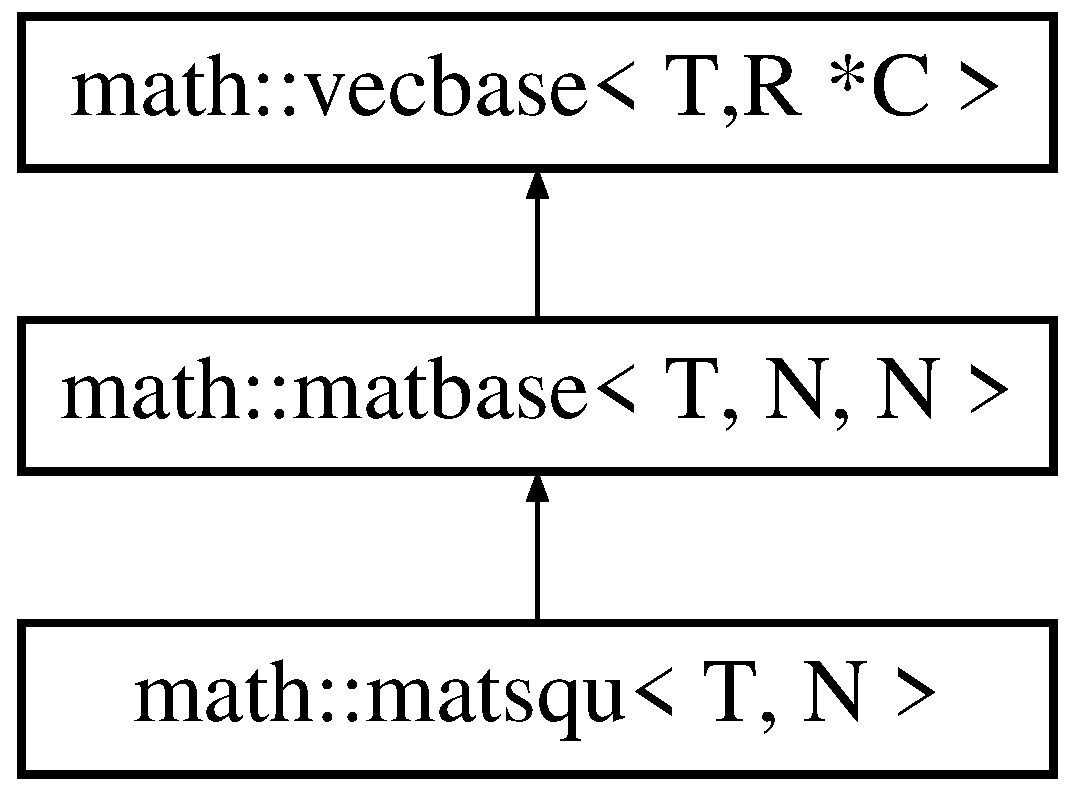
\includegraphics[height=3cm]{classmath_1_1matsqu}
\end{center}
\end{figure}
\subsection*{Public Member Functions}
\begin{DoxyCompactItemize}
\item 
\hypertarget{classmath_1_1matsqu_a04647ad3f7539a9aac5654a2e569682a}{
T \hyperlink{classmath_1_1matsqu_a04647ad3f7539a9aac5654a2e569682a}{det} ()}
\label{classmath_1_1matsqu_a04647ad3f7539a9aac5654a2e569682a}

\begin{DoxyCompactList}\small\item\em determinant \item\end{DoxyCompactList}\item 
\hypertarget{classmath_1_1matsqu_a5a63541112ab40372e761931e7843727}{
T \hyperlink{classmath_1_1matsqu_a5a63541112ab40372e761931e7843727}{det} (int $\ast$a, int $\ast$b, int n)}
\label{classmath_1_1matsqu_a5a63541112ab40372e761931e7843727}

\begin{DoxyCompactList}\small\item\em determinant of subset \item\end{DoxyCompactList}\end{DoxyCompactItemize}
\subsubsection*{template$<$typename T, int N$>$ class math::matsqu$<$ T, N $>$}



The documentation for this class was generated from the following file:\begin{DoxyCompactItemize}
\item 
src/math/vecbase.hpp\end{DoxyCompactItemize}

\hypertarget{classmath_1_1discrete_1_1Graph_1_1Node}{
\section{math::discrete::Graph::Node Class Reference}
\label{classmath_1_1discrete_1_1Graph_1_1Node}\index{math::discrete::Graph::Node@{math::discrete::Graph::Node}}
}


The documentation for this class was generated from the following file:\begin{DoxyCompactItemize}
\item 
src/math/discrete/discrete.hpp\end{DoxyCompactItemize}

\hypertarget{classmath_1_1plane}{
\section{math::plane Class Reference}
\label{classmath_1_1plane}\index{math::plane@{math::plane}}
}
\subsection*{Public Types}
\begin{DoxyCompactItemize}
\item 
enum \{ {\bfseries POINT\_\-ON\_\-PLANE} = 0, 
{\bfseries POINT\_\-IN\_\-FRONT\_\-OF\_\-PLANE} = 1, 
{\bfseries POINT\_\-BEHIND\_\-PLANE} = 2
 \}
\end{DoxyCompactItemize}
\subsection*{Public Member Functions}
\begin{DoxyCompactItemize}
\item 
\hypertarget{classmath_1_1plane_afebf782c7828f4f6c53462b0a9b18b1e}{
{\bfseries plane} (\hyperlink{classmath_1_1vec3}{vec3} newNormal, float newIntercept)}
\label{classmath_1_1plane_afebf782c7828f4f6c53462b0a9b18b1e}

\item 
\hypertarget{classmath_1_1plane_a25c3bf9902eaff31c6b5bbf9a1b3322a}{
{\bfseries plane} (const \hyperlink{classmath_1_1plane}{plane} \&rhs)}
\label{classmath_1_1plane_a25c3bf9902eaff31c6b5bbf9a1b3322a}

\item 
\hypertarget{classmath_1_1plane_a9fe8b3594923c703c1ab5c644a7fba60}{
void {\bfseries SetNormal} (const \hyperlink{classmath_1_1vec3}{vec3} \&rhs)}
\label{classmath_1_1plane_a9fe8b3594923c703c1ab5c644a7fba60}

\item 
\hypertarget{classmath_1_1plane_a7ed123f20808367fbeda9e75eaaa6766}{
void {\bfseries SetIntercept} (float newIntercept)}
\label{classmath_1_1plane_a7ed123f20808367fbeda9e75eaaa6766}

\item 
\hypertarget{classmath_1_1plane_a39bd4a07bf6b7b4583d522ff11f873d0}{
void {\bfseries SetFromPoints} (const \hyperlink{classmath_1_1vec3}{vec3} \&p0, const \hyperlink{classmath_1_1vec3}{vec3} \&p1, const \hyperlink{classmath_1_1vec3}{vec3} \&p2)}
\label{classmath_1_1plane_a39bd4a07bf6b7b4583d522ff11f873d0}

\item 
\hypertarget{classmath_1_1plane_ae4275e2af7ccdacaf4a3e0831ea009cc}{
void {\bfseries CalculateIntercept} (const \hyperlink{classmath_1_1vec3}{vec3} \&pointOnPlane)}
\label{classmath_1_1plane_ae4275e2af7ccdacaf4a3e0831ea009cc}

\item 
\hypertarget{classmath_1_1plane_afea36d03496c252a22b98506d33117df}{
void {\bfseries Normalize} (void)}
\label{classmath_1_1plane_afea36d03496c252a22b98506d33117df}

\item 
\hypertarget{classmath_1_1plane_a21aeb399211c8e50a391ce70bb71a113}{
\hyperlink{classmath_1_1vec3}{vec3} {\bfseries GetNormal} ()}
\label{classmath_1_1plane_a21aeb399211c8e50a391ce70bb71a113}

\item 
\hypertarget{classmath_1_1plane_ac8127f9e5b508ba2c51a3422122c2511}{
float {\bfseries GetIntercept} ()}
\label{classmath_1_1plane_ac8127f9e5b508ba2c51a3422122c2511}

\item 
\hypertarget{classmath_1_1plane_af6f50a2db368dced1ae9572422d6d7e2}{
bool {\bfseries Intersect3} (const \hyperlink{classmath_1_1plane}{plane} \&p2, const \hyperlink{classmath_1_1plane}{plane} \&p3, \hyperlink{classmath_1_1vec3}{vec3} \&result)}
\label{classmath_1_1plane_af6f50a2db368dced1ae9572422d6d7e2}

\item 
\hypertarget{classmath_1_1plane_ab27db4ca27caec4dd84311483ba65c23}{
float {\bfseries GetDistance} (const \hyperlink{classmath_1_1vec3}{vec3} \&point) const }
\label{classmath_1_1plane_ab27db4ca27caec4dd84311483ba65c23}

\item 
\hypertarget{classmath_1_1plane_af3871a442fb338ab1524f96d9956b68f}{
int {\bfseries ClassifyPoint} (const \hyperlink{classmath_1_1vec3}{vec3} \&point) const }
\label{classmath_1_1plane_af3871a442fb338ab1524f96d9956b68f}

\item 
\hypertarget{classmath_1_1plane_affa8cd87ad8b3da63511d526fd81a1a6}{
\hyperlink{classmath_1_1plane}{plane} {\bfseries lerp} (const \hyperlink{classmath_1_1plane}{plane} \&p2, float factor)}
\label{classmath_1_1plane_affa8cd87ad8b3da63511d526fd81a1a6}

\item 
\hypertarget{classmath_1_1plane_ac5c24435016da495c52e9a7ca9cc1f08}{
bool {\bfseries operator==} (const \hyperlink{classmath_1_1plane}{plane} \&rhs) const }
\label{classmath_1_1plane_ac5c24435016da495c52e9a7ca9cc1f08}

\item 
\hypertarget{classmath_1_1plane_a45108625f3dc606b7df31386cce2f1c2}{
bool {\bfseries operator!=} (const \hyperlink{classmath_1_1plane}{plane} \&rhs) const }
\label{classmath_1_1plane_a45108625f3dc606b7df31386cce2f1c2}

\item 
\hypertarget{classmath_1_1plane_a4c9f64519742f6d7d0370a62101733c4}{
\hyperlink{classmath_1_1plane}{plane} {\bfseries operator-\/} (void) const }
\label{classmath_1_1plane_a4c9f64519742f6d7d0370a62101733c4}

\item 
\hypertarget{classmath_1_1plane_a57123617c9e3bfaed24cc655205b17ed}{
\hyperlink{classmath_1_1plane}{plane} {\bfseries operator+} (void) const }
\label{classmath_1_1plane_a57123617c9e3bfaed24cc655205b17ed}

\end{DoxyCompactItemize}
\subsection*{Public Attributes}
\begin{DoxyCompactItemize}
\item 
\hypertarget{classmath_1_1plane_aa4e78c5134a44175182b2f955e57d0f0}{
\hyperlink{classmath_1_1vec3}{vec3} {\bfseries n}}
\label{classmath_1_1plane_aa4e78c5134a44175182b2f955e57d0f0}

\item 
\hypertarget{classmath_1_1plane_a20a1f2d1caa4d5cb3d81f779bb4572b0}{
float {\bfseries d}}
\label{classmath_1_1plane_a20a1f2d1caa4d5cb3d81f779bb4572b0}

\end{DoxyCompactItemize}


The documentation for this class was generated from the following files:\begin{DoxyCompactItemize}
\item 
src/math/plane.h\item 
src/math/plane.cpp\end{DoxyCompactItemize}

\hypertarget{classplane}{
\section{plane Class Reference}
\label{classplane}\index{plane@{plane}}
}
\subsection*{Public Member Functions}
\begin{DoxyCompactItemize}
\item 
\hypertarget{classplane_a86ba049725c9bd1993d4412c29a12771}{
{\bfseries plane} (\hyperlink{classfeature}{feature} $\ast$feat0, \hyperlink{classfeature}{feature} $\ast$feat1)}
\label{classplane_a86ba049725c9bd1993d4412c29a12771}

\item 
\hypertarget{classplane_ad55d61ae11dfdafe52127f725b844fda}{
float {\bfseries dist} (\hyperlink{classmath_1_1vec3}{math::vec3} v)}
\label{classplane_ad55d61ae11dfdafe52127f725b844fda}

\end{DoxyCompactItemize}
\subsection*{Public Attributes}
\begin{DoxyCompactItemize}
\item 
\hypertarget{classplane_a2abd702f2868e2b7ca6fd36378462b8d}{
\hyperlink{classmath_1_1vec3}{math::vec3} {\bfseries n}}
\label{classplane_a2abd702f2868e2b7ca6fd36378462b8d}

\end{DoxyCompactItemize}


The documentation for this class was generated from the following file:\begin{DoxyCompactItemize}
\item 
src/math/vclip/vclip.h\end{DoxyCompactItemize}

\hypertarget{classmath_1_1geo_1_1polygon}{
\section{math::geo::polygon Class Reference}
\label{classmath_1_1geo_1_1polygon}\index{math::geo::polygon@{math::geo::polygon}}
}


The documentation for this class was generated from the following file:\begin{DoxyCompactItemize}
\item 
src/math/geo/polyhedron.hpp\end{DoxyCompactItemize}

\hypertarget{classpolyhedron}{
\section{polyhedron Class Reference}
\label{classpolyhedron}\index{polyhedron@{polyhedron}}
}
\subsection*{Public Attributes}
\begin{DoxyCompactItemize}
\item 
\hypertarget{classpolyhedron_abfafc703e4310ed74d41261c72cd0530}{
std::set$<$ \hyperlink{classface}{face} $\ast$ $>$ {\bfseries f}}
\label{classpolyhedron_abfafc703e4310ed74d41261c72cd0530}

\end{DoxyCompactItemize}


The documentation for this class was generated from the following file:\begin{DoxyCompactItemize}
\item 
src/math/vclip/vclip.hpp\end{DoxyCompactItemize}

\hypertarget{classmath_1_1geo_1_1polyhedron}{
\section{math::geo::polyhedron Class Reference}
\label{classmath_1_1geo_1_1polyhedron}\index{math::geo::polyhedron@{math::geo::polyhedron}}
}
Inheritance diagram for math::geo::polyhedron::\begin{figure}[H]
\begin{center}
\leavevmode
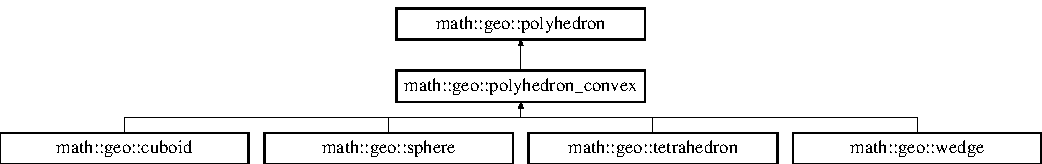
\includegraphics[height=2.19895cm]{classmath_1_1geo_1_1polyhedron}
\end{center}
\end{figure}
\subsection*{Public Types}
\begin{DoxyCompactItemize}
\item 
enum \{ {\bfseries PER\_\-FACE\_\-NORMAL}
 \}
\end{DoxyCompactItemize}
\subsection*{Public Attributes}
\begin{DoxyCompactItemize}
\item 
\hypertarget{classmath_1_1geo_1_1polyhedron_a95b429bd2b0b049560fc008563663b17}{
\hyperlink{classmath_1_1geo_1_1vertex}{vertex} $\ast$ {\bfseries vertices\_\-}}
\label{classmath_1_1geo_1_1polyhedron_a95b429bd2b0b049560fc008563663b17}

\item 
\hypertarget{classmath_1_1geo_1_1polyhedron_a1f3a59fa6add8c59eea9deea460c3c96}{
\hyperlink{classmath_1_1geo_1_1tri}{tri} $\ast$ {\bfseries tris\_\-}}
\label{classmath_1_1geo_1_1polyhedron_a1f3a59fa6add8c59eea9deea460c3c96}

\item 
\hypertarget{classmath_1_1geo_1_1polyhedron_aece41abb7f5005d9ff6de2016aae790c}{
\hyperlink{classmath_1_1geo_1_1quad}{quad} $\ast$ {\bfseries quads\_\-}}
\label{classmath_1_1geo_1_1polyhedron_aece41abb7f5005d9ff6de2016aae790c}

\item 
\hypertarget{classmath_1_1geo_1_1polyhedron_ab8bbfdd91290c53d8f8e0c55c3f11fdd}{
int {\bfseries nt\_\-}}
\label{classmath_1_1geo_1_1polyhedron_ab8bbfdd91290c53d8f8e0c55c3f11fdd}

\item 
\hypertarget{classmath_1_1geo_1_1polyhedron_ac5bbb1b818226c30b4f8ea39006efa57}{
int {\bfseries nq\_\-}}
\label{classmath_1_1geo_1_1polyhedron_ac5bbb1b818226c30b4f8ea39006efa57}

\item 
\hypertarget{classmath_1_1geo_1_1polyhedron_a962cdc8309c56bd40a34c3af223d6fd3}{
unsigned int {\bfseries flag\_\-}}
\label{classmath_1_1geo_1_1polyhedron_a962cdc8309c56bd40a34c3af223d6fd3}

\end{DoxyCompactItemize}


The documentation for this class was generated from the following file:\begin{DoxyCompactItemize}
\item 
src/math/geo/polyhedron.hpp\end{DoxyCompactItemize}

\hypertarget{classmath_1_1geo_1_1polyhedron__convex}{
\section{math::geo::polyhedron\_\-convex Class Reference}
\label{classmath_1_1geo_1_1polyhedron__convex}\index{math::geo::polyhedron\_\-convex@{math::geo::polyhedron\_\-convex}}
}
Inheritance diagram for math::geo::polyhedron\_\-convex::\begin{figure}[H]
\begin{center}
\leavevmode
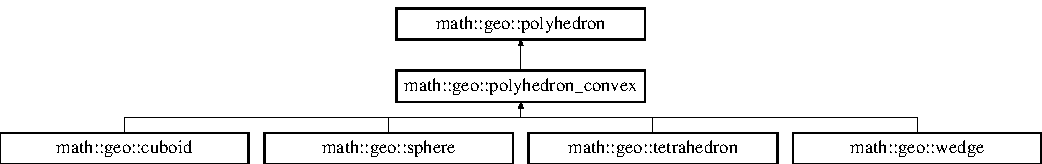
\includegraphics[height=2.19895cm]{classmath_1_1geo_1_1polyhedron__convex}
\end{center}
\end{figure}


The documentation for this class was generated from the following file:\begin{DoxyCompactItemize}
\item 
src/math/geo/polyhedron.hpp\end{DoxyCompactItemize}

\hypertarget{classmath_1_1polynomial}{
\section{math::polynomial Class Reference}
\label{classmath_1_1polynomial}\index{math::polynomial@{math::polynomial}}
}
\subsection*{Public Attributes}
\begin{DoxyCompactItemize}
\item 
\hypertarget{classmath_1_1polynomial_ab2a0a58ff9c7a98300265bce13c88daa}{
float $\ast$ {\bfseries a}}
\label{classmath_1_1polynomial_ab2a0a58ff9c7a98300265bce13c88daa}

\item 
\hypertarget{classmath_1_1polynomial_ad296013c1a1174bb85ee013a1f6139fa}{
int {\bfseries n}}
\label{classmath_1_1polynomial_ad296013c1a1174bb85ee013a1f6139fa}

\end{DoxyCompactItemize}


The documentation for this class was generated from the following file:\begin{DoxyCompactItemize}
\item 
src/math/polynomial.hpp\end{DoxyCompactItemize}

\hypertarget{classmath_1_1geo_1_1quad}{
\section{math::geo::quad Class Reference}
\label{classmath_1_1geo_1_1quad}\index{math::geo::quad@{math::geo::quad}}
}
\subsection*{Public Member Functions}
\begin{DoxyCompactItemize}
\item 
\hypertarget{classmath_1_1geo_1_1quad_a61f7422d3d82b7acab0aabd71b68fccf}{
void {\bfseries reset\_\-normals} ()}
\label{classmath_1_1geo_1_1quad_a61f7422d3d82b7acab0aabd71b68fccf}

\end{DoxyCompactItemize}
\subsection*{Public Attributes}
\begin{DoxyCompactItemize}
\item 
\hypertarget{classmath_1_1geo_1_1quad_a6625bbd8467b8a853aae1f4f2a2362ec}{
\hyperlink{classmath_1_1geo_1_1vertex}{vertex} {\bfseries v\_\-} \mbox{[}4\mbox{]}}
\label{classmath_1_1geo_1_1quad_a6625bbd8467b8a853aae1f4f2a2362ec}

\end{DoxyCompactItemize}


The documentation for this class was generated from the following file:\begin{DoxyCompactItemize}
\item 
src/math/geo/polyhedron.hpp\end{DoxyCompactItemize}

\hypertarget{classmath_1_1quat}{
\section{math::quat Class Reference}
\label{classmath_1_1quat}\index{math::quat@{math::quat}}
}
\subsection*{Public Member Functions}
\begin{DoxyCompactItemize}
\item 
\hypertarget{classmath_1_1quat_abd5d4e621692f255903b6774ded20d55}{
{\bfseries quat} (double nx, double ny, double nz, double nw)}
\label{classmath_1_1quat_abd5d4e621692f255903b6774ded20d55}

\item 
\hypertarget{classmath_1_1quat_a3c52efa70f7438fc36f5320e6c36b541}{
{\bfseries quat} (double angleRadians, \hyperlink{classmath_1_1vec3}{vec3}$<$ double $>$ const \&axis)}
\label{classmath_1_1quat_a3c52efa70f7438fc36f5320e6c36b541}

\item 
\hypertarget{classmath_1_1quat_adee27ee6bd123e700f938c4933e5193d}{
{\bfseries quat} (\hyperlink{classmath_1_1quat}{quat} const \&v)}
\label{classmath_1_1quat_adee27ee6bd123e700f938c4933e5193d}

\item 
\hypertarget{classmath_1_1quat_ab3c6f06cfc6ad9aab7bb34205dbbe9a2}{
{\bfseries quat} (\hyperlink{classmath_1_1vec3}{vec3}$<$ double $>$ const \&, \hyperlink{classmath_1_1vec3}{vec3}$<$ double $>$ const \&)}
\label{classmath_1_1quat_ab3c6f06cfc6ad9aab7bb34205dbbe9a2}

\item 
\hypertarget{classmath_1_1quat_ae4b41838614ed4470ede0f8895b844f1}{
{\bfseries quat} (\hyperlink{classmath_1_1mat44}{mat44} const \&m)}
\label{classmath_1_1quat_ae4b41838614ed4470ede0f8895b844f1}

\item 
\hypertarget{classmath_1_1quat_a40a99cdc7e0dd1325367cebfe08b98d7}{
void {\bfseries loadZero} ()}
\label{classmath_1_1quat_a40a99cdc7e0dd1325367cebfe08b98d7}

\item 
\hypertarget{classmath_1_1quat_a3246b760dcd8bc3ac5e46292659e8421}{
bool {\bfseries isFinite} () const }
\label{classmath_1_1quat_a3246b760dcd8bc3ac5e46292659e8421}

\item 
\hypertarget{classmath_1_1quat_a41549edf9f8204cc7a083c2db1940ad0}{
bool \hyperlink{classmath_1_1quat_a41549edf9f8204cc7a083c2db1940ad0}{isUnit} () const }
\label{classmath_1_1quat_a41549edf9f8204cc7a083c2db1940ad0}

\begin{DoxyCompactList}\small\item\em returns true if finite and magnitude is close to unit \item\end{DoxyCompactList}\item 
\hypertarget{classmath_1_1quat_a1ba9cba4f4688f2e82de0078af1bcf52}{
bool \hyperlink{classmath_1_1quat_a1ba9cba4f4688f2e82de0078af1bcf52}{isSane} () const }
\label{classmath_1_1quat_a1ba9cba4f4688f2e82de0078af1bcf52}

\begin{DoxyCompactList}\small\item\em returns true if finite and magnitude is reasonably close to unit to allow for some accumulation of error vs isValid \item\end{DoxyCompactList}\item 
\hypertarget{classmath_1_1quat_acf30faafb93a587a99fe6d2f99c24a45}{
void \hyperlink{classmath_1_1quat_acf30faafb93a587a99fe6d2f99c24a45}{toRadiansAndUnitAxis} (double \&angle, \hyperlink{classmath_1_1vec3}{vec3}$<$ double $>$ \&axis) const }
\label{classmath_1_1quat_acf30faafb93a587a99fe6d2f99c24a45}

\begin{DoxyCompactList}\small\item\em converts this quaternion to angle-\/axis representation \item\end{DoxyCompactList}\item 
\hypertarget{classmath_1_1quat_a9c5919a9230a3207663b2da1f982a714}{
double {\bfseries getAngle} () const }
\label{classmath_1_1quat_a9c5919a9230a3207663b2da1f982a714}

\item 
\hypertarget{classmath_1_1quat_a22f97cf89cb83fbdeddbcdf7cd360f4f}{
double {\bfseries getAngle} (const \hyperlink{classmath_1_1quat}{quat} \&q) const }
\label{classmath_1_1quat_a22f97cf89cb83fbdeddbcdf7cd360f4f}

\item 
\hypertarget{classmath_1_1quat_abe53d7e37a35f982393d8c1b7c0d9397}{
double {\bfseries magnitudeSquared} () const }
\label{classmath_1_1quat_abe53d7e37a35f982393d8c1b7c0d9397}

\item 
\hypertarget{classmath_1_1quat_a559847bc6ecc61f2315d21bf5d56abb5}{
double {\bfseries dot} (const \hyperlink{classmath_1_1quat}{quat} \&v) const }
\label{classmath_1_1quat_a559847bc6ecc61f2315d21bf5d56abb5}

\item 
\hypertarget{classmath_1_1quat_aa3d1bb2f539e50c692f955f40e05bd23}{
\hyperlink{classmath_1_1quat}{quat} {\bfseries getNormalized} () const }
\label{classmath_1_1quat_aa3d1bb2f539e50c692f955f40e05bd23}

\item 
\hypertarget{classmath_1_1quat_afc9da36b57a5fd6f678ce0b5acd10fee}{
double {\bfseries magnitude} () const }
\label{classmath_1_1quat_afc9da36b57a5fd6f678ce0b5acd10fee}

\item 
\hypertarget{classmath_1_1quat_a1ba0f12c4c6b8cc2090b4d5ea91e39a2}{
double {\bfseries normalize} ()}
\label{classmath_1_1quat_a1ba0f12c4c6b8cc2090b4d5ea91e39a2}

\item 
\hypertarget{classmath_1_1quat_aaa518b97b4b1de62a2bf341239061b08}{
\hyperlink{classmath_1_1quat}{quat} {\bfseries getConjugate} () const }
\label{classmath_1_1quat_aaa518b97b4b1de62a2bf341239061b08}

\item 
\hypertarget{classmath_1_1quat_a6e6d2a97e1fc2e75385702f96ea8644e}{
\hyperlink{classmath_1_1vec3}{vec3}$<$ double $>$ {\bfseries getImaginaryPart} () const }
\label{classmath_1_1quat_a6e6d2a97e1fc2e75385702f96ea8644e}

\item 
\hypertarget{classmath_1_1quat_a3ee5806c2c8003c20b8accd50f2b8514}{
\hyperlink{classmath_1_1vec3}{vec3}$<$ double $>$ {\bfseries getBasisVector0} () const }
\label{classmath_1_1quat_a3ee5806c2c8003c20b8accd50f2b8514}

\item 
\hypertarget{classmath_1_1quat_a486e21af4f600a4f2d972cc782c92f47}{
\hyperlink{classmath_1_1vec3}{vec3}$<$ double $>$ {\bfseries getBasisVector1} () const }
\label{classmath_1_1quat_a486e21af4f600a4f2d972cc782c92f47}

\item 
\hypertarget{classmath_1_1quat_a4d96d1cec1f48b5e6c76e1b6fd84084e}{
\hyperlink{classmath_1_1vec3}{vec3}$<$ double $>$ {\bfseries getBasisVector2} () const }
\label{classmath_1_1quat_a4d96d1cec1f48b5e6c76e1b6fd84084e}

\item 
\hypertarget{classmath_1_1quat_a6c3e3277474838d174a45d61a776c797}{
const \hyperlink{classmath_1_1vec3}{vec3}$<$ double $>$ {\bfseries rotate} (const \hyperlink{classmath_1_1vec3}{vec3}$<$ double $>$ \&v) const }
\label{classmath_1_1quat_a6c3e3277474838d174a45d61a776c797}

\item 
\hypertarget{classmath_1_1quat_a42f50c4378af552d28e761f8c3e884a9}{
const \hyperlink{classmath_1_1vec3}{vec3}$<$ double $>$ {\bfseries rotateInv} (const \hyperlink{classmath_1_1vec3}{vec3}$<$ double $>$ \&v) const }
\label{classmath_1_1quat_a42f50c4378af552d28e761f8c3e884a9}

\item 
\hypertarget{classmath_1_1quat_a1ed0d2c147ecb5ac5c883de8a5b8dcda}{
\hyperlink{classmath_1_1quat}{quat} \& {\bfseries operator=} (const \hyperlink{classmath_1_1quat}{quat} \&p)}
\label{classmath_1_1quat_a1ed0d2c147ecb5ac5c883de8a5b8dcda}

\item 
\hypertarget{classmath_1_1quat_a5a91d5ac36d622a38019d251fa36052e}{
\hyperlink{classmath_1_1quat}{quat} \& {\bfseries operator$\ast$=} (const \hyperlink{classmath_1_1quat}{quat} \&q)}
\label{classmath_1_1quat_a5a91d5ac36d622a38019d251fa36052e}

\item 
\hypertarget{classmath_1_1quat_a726b3d1a6b752825275640b9be95e146}{
\hyperlink{classmath_1_1quat}{quat} \& {\bfseries operator+=} (const \hyperlink{classmath_1_1quat}{quat} \&q)}
\label{classmath_1_1quat_a726b3d1a6b752825275640b9be95e146}

\item 
\hypertarget{classmath_1_1quat_a00756143601dc92e5762e3321a3ef3b6}{
\hyperlink{classmath_1_1quat}{quat} \& {\bfseries operator-\/=} (const \hyperlink{classmath_1_1quat}{quat} \&q)}
\label{classmath_1_1quat_a00756143601dc92e5762e3321a3ef3b6}

\item 
\hypertarget{classmath_1_1quat_a90295c24018c6b84b88a682b5384db3e}{
\hyperlink{classmath_1_1quat}{quat} \& {\bfseries operator$\ast$=} (const double s)}
\label{classmath_1_1quat_a90295c24018c6b84b88a682b5384db3e}

\item 
\hypertarget{classmath_1_1quat_a55ebbe795c43772d6b7d7958910b0fa4}{
\hyperlink{classmath_1_1quat}{quat} {\bfseries operator$\ast$} (const \hyperlink{classmath_1_1quat}{quat} \&q) const }
\label{classmath_1_1quat_a55ebbe795c43772d6b7d7958910b0fa4}

\item 
\hypertarget{classmath_1_1quat_abe6847bb92a612e5e0182477fd7a4791}{
\hyperlink{classmath_1_1quat}{quat} {\bfseries operator+} (const \hyperlink{classmath_1_1quat}{quat} \&q) const }
\label{classmath_1_1quat_abe6847bb92a612e5e0182477fd7a4791}

\item 
\hypertarget{classmath_1_1quat_a180b5c18159637593b0d67d39bb2a0c8}{
\hyperlink{classmath_1_1quat}{quat} {\bfseries operator-\/} () const }
\label{classmath_1_1quat_a180b5c18159637593b0d67d39bb2a0c8}

\item 
\hypertarget{classmath_1_1quat_ab63582f1e6470c0e194d0e3a56e877a4}{
\hyperlink{classmath_1_1quat}{quat} {\bfseries operator-\/} (const \hyperlink{classmath_1_1quat}{quat} \&q) const }
\label{classmath_1_1quat_ab63582f1e6470c0e194d0e3a56e877a4}

\item 
\hypertarget{classmath_1_1quat_a3347486321da83dc25efc23bacc88978}{
\hyperlink{classmath_1_1quat}{quat} {\bfseries operator$\ast$} (double r) const }
\label{classmath_1_1quat_a3347486321da83dc25efc23bacc88978}

\item 
\hypertarget{classmath_1_1quat_a74566738661524ff50eccf6a5b8034f9}{
\hyperlink{classmath_1_1vec3}{vec3}$<$ double $>$ {\bfseries getOmega} (double dt)}
\label{classmath_1_1quat_a74566738661524ff50eccf6a5b8034f9}

\item 
\hypertarget{classmath_1_1quat_adf904d1bde884ccea84e06b4498d8d10}{
void {\bfseries print} ()}
\label{classmath_1_1quat_adf904d1bde884ccea84e06b4498d8d10}

\end{DoxyCompactItemize}
\subsection*{Static Public Member Functions}
\begin{DoxyCompactItemize}
\item 
\hypertarget{classmath_1_1quat_a8eda07c74adf541d6196b900aa36cb02}{
static \hyperlink{classmath_1_1quat}{quat} {\bfseries createIdentity} ()}
\label{classmath_1_1quat_a8eda07c74adf541d6196b900aa36cb02}

\end{DoxyCompactItemize}
\subsection*{Public Attributes}
\begin{DoxyCompactItemize}
\item 
\hypertarget{classmath_1_1quat_a5f5eb994694bfb16fffc1bbfa8865305}{
double {\bfseries w}}
\label{classmath_1_1quat_a5f5eb994694bfb16fffc1bbfa8865305}

\item 
\hypertarget{classmath_1_1quat_a344e9a3322595602c0d27d410ab5e0e4}{
double {\bfseries x}}
\label{classmath_1_1quat_a344e9a3322595602c0d27d410ab5e0e4}

\item 
\hypertarget{classmath_1_1quat_a270052a715675dce2740c9e29db72297}{
double {\bfseries y}}
\label{classmath_1_1quat_a270052a715675dce2740c9e29db72297}

\item 
\hypertarget{classmath_1_1quat_a3a9fb8daa232089f7410d91ee2fd2d65}{
double {\bfseries z}}
\label{classmath_1_1quat_a3a9fb8daa232089f7410d91ee2fd2d65}

\end{DoxyCompactItemize}


The documentation for this class was generated from the following files:\begin{DoxyCompactItemize}
\item 
src/math/quat.h\item 
src/math/quat.cpp\end{DoxyCompactItemize}

\hypertarget{classmath_1_1geo_1_1sphere}{
\section{math::geo::sphere Class Reference}
\label{classmath_1_1geo_1_1sphere}\index{math::geo::sphere@{math::geo::sphere}}
}
Inheritance diagram for math::geo::sphere::\begin{figure}[H]
\begin{center}
\leavevmode
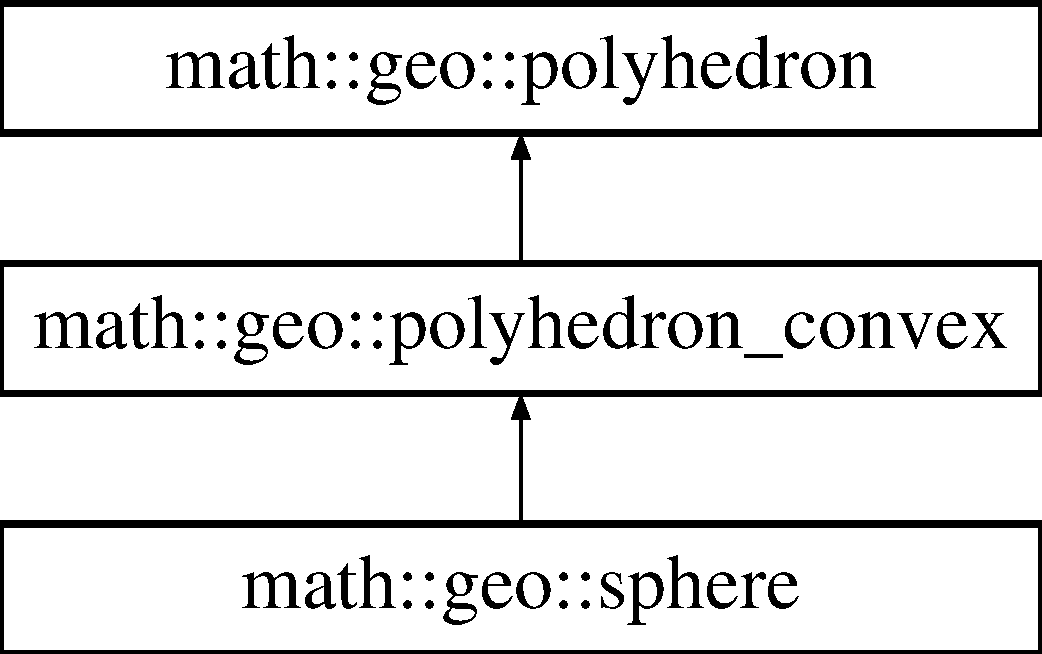
\includegraphics[height=3cm]{classmath_1_1geo_1_1sphere}
\end{center}
\end{figure}
\subsection*{Public Member Functions}
\begin{DoxyCompactItemize}
\item 
\hypertarget{classmath_1_1geo_1_1sphere_ad30f9edddc96ef9c7a4062e79694556d}{
{\bfseries sphere} (float, int, int)}
\label{classmath_1_1geo_1_1sphere_ad30f9edddc96ef9c7a4062e79694556d}

\end{DoxyCompactItemize}


The documentation for this class was generated from the following files:\begin{DoxyCompactItemize}
\item 
src/math/geo/polyhedron.hpp\item 
src/math/geo/polyhedron.cpp\end{DoxyCompactItemize}

\hypertarget{classmath_1_1geo_1_1tetrahedron}{
\section{math::geo::tetrahedron Class Reference}
\label{classmath_1_1geo_1_1tetrahedron}\index{math::geo::tetrahedron@{math::geo::tetrahedron}}
}
Inheritance diagram for math::geo::tetrahedron::\begin{figure}[H]
\begin{center}
\leavevmode
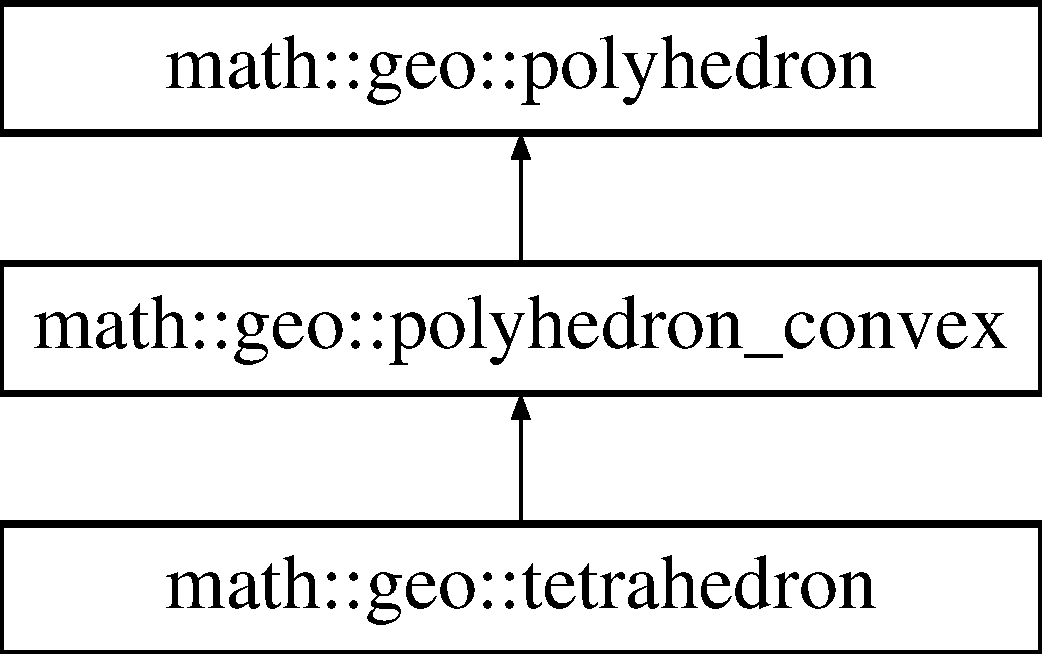
\includegraphics[height=3cm]{classmath_1_1geo_1_1tetrahedron}
\end{center}
\end{figure}


The documentation for this class was generated from the following file:\begin{DoxyCompactItemize}
\item 
src/math/geo/polyhedron.hpp\end{DoxyCompactItemize}

\hypertarget{classmath_1_1transform}{
\section{math::transform$<$ T $>$ Class Template Reference}
\label{classmath_1_1transform}\index{math::transform@{math::transform}}
}
\subsection*{Public Member Functions}
\begin{DoxyCompactItemize}
\item 
\hypertarget{classmath_1_1transform_ac9ae83b2a4856b0763d6e845c2cd60a0}{
\hyperlink{classmath_1_1transform}{transform} {\bfseries operator$\ast$} (const \hyperlink{classmath_1_1transform}{transform} \&x) const }
\label{classmath_1_1transform_ac9ae83b2a4856b0763d6e845c2cd60a0}

\item 
\hypertarget{classmath_1_1transform_a64e208d96af2e40311962c718d06a253}{
\hyperlink{classmath_1_1transform}{transform} {\bfseries getInverse} () const }
\label{classmath_1_1transform_a64e208d96af2e40311962c718d06a253}

\item 
\hypertarget{classmath_1_1transform_a4ed85416967cc655ab18db6049cd0c9a}{
\hyperlink{classmath_1_1vec3}{vec3}$<$ double $>$ {\bfseries trans} (const \hyperlink{classmath_1_1vec3}{vec3}$<$ double $>$ \&input) const }
\label{classmath_1_1transform_a4ed85416967cc655ab18db6049cd0c9a}

\item 
\hypertarget{classmath_1_1transform_a783e2f24598656c2e696c4dab8a1b6b9}{
\hyperlink{classmath_1_1vec3}{vec3}$<$ double $>$ {\bfseries transInv} (const \hyperlink{classmath_1_1vec3}{vec3}$<$ double $>$ \&input) const }
\label{classmath_1_1transform_a783e2f24598656c2e696c4dab8a1b6b9}

\item 
\hypertarget{classmath_1_1transform_ae1dc64bee8360e3c8cf52989555da8af}{
\hyperlink{classmath_1_1vec3}{vec3}$<$ double $>$ {\bfseries rotate} (const \hyperlink{classmath_1_1vec3}{vec3}$<$ double $>$ \&input) const }
\label{classmath_1_1transform_ae1dc64bee8360e3c8cf52989555da8af}

\item 
\hypertarget{classmath_1_1transform_a845be40f034a7d35d0ab6298f734bea5}{
\hyperlink{classmath_1_1vec3}{vec3}$<$ double $>$ {\bfseries rotateInv} (const \hyperlink{classmath_1_1vec3}{vec3}$<$ double $>$ \&input) const }
\label{classmath_1_1transform_a845be40f034a7d35d0ab6298f734bea5}

\item 
\hypertarget{classmath_1_1transform_aac85fac3bbd90679a2d43511f24bdd42}{
\hyperlink{classmath_1_1transform}{transform} {\bfseries trans} (const \hyperlink{classmath_1_1transform}{transform} \&src) const }
\label{classmath_1_1transform_aac85fac3bbd90679a2d43511f24bdd42}

\item 
\hypertarget{classmath_1_1transform_ac31f73479d89e0401f44b59b243ddacd}{
bool {\bfseries isValid} () const }
\label{classmath_1_1transform_ac31f73479d89e0401f44b59b243ddacd}

\item 
\hypertarget{classmath_1_1transform_a7a6602be4a1c9eb4fb20514c5eee965b}{
bool {\bfseries isSane} () const }
\label{classmath_1_1transform_a7a6602be4a1c9eb4fb20514c5eee965b}

\item 
\hypertarget{classmath_1_1transform_a92670298b2affc9daf52716076d6cbdc}{
bool {\bfseries isFinite} () const }
\label{classmath_1_1transform_a92670298b2affc9daf52716076d6cbdc}

\item 
\hypertarget{classmath_1_1transform_aafec67428664ec08699ed2b06ffec04a}{
\hyperlink{classmath_1_1transform}{transform} {\bfseries transformInv} (const \hyperlink{classmath_1_1transform}{transform} \&src) const }
\label{classmath_1_1transform_aafec67428664ec08699ed2b06ffec04a}

\item 
\hypertarget{classmath_1_1transform_a22d5670f272e14ba4a392220a6d9fbc4}{
\hyperlink{classmath_1_1transform}{transform} {\bfseries getNormalized} () const }
\label{classmath_1_1transform_a22d5670f272e14ba4a392220a6d9fbc4}

\end{DoxyCompactItemize}
\begin{Indent}{\bf Constructors}\par
{\em \label{_amgrp559a25fdb98a7d1fd1c3771ac568d5e9}
 }\begin{DoxyCompactItemize}
\item 
\hypertarget{classmath_1_1transform_aac5c96a861fd0efa2f59b934aa18209b}{
{\bfseries transform} ()}
\label{classmath_1_1transform_aac5c96a861fd0efa2f59b934aa18209b}

\item 
\hypertarget{classmath_1_1transform_aecf7886adfe7f3a7106cd447fea3e185}{
{\bfseries transform} (\hyperlink{classmath_1_1vec3}{vec3}$<$ T $>$ const \&np)}
\label{classmath_1_1transform_aecf7886adfe7f3a7106cd447fea3e185}

\item 
\hypertarget{classmath_1_1transform_ae93a4f522574b2b1e7445aa3f6098a9e}{
{\bfseries transform} (\hyperlink{classmath_1_1quat}{quat}$<$ T $>$ const \&nq)}
\label{classmath_1_1transform_ae93a4f522574b2b1e7445aa3f6098a9e}

\item 
\hypertarget{classmath_1_1transform_af6b5742b9215436c87770a970456265a}{
{\bfseries transform} (\hyperlink{classmath_1_1vec3}{vec3}$<$ T $>$const \&np, \hyperlink{classmath_1_1quat}{quat}$<$ T $>$ const \&nq)}
\label{classmath_1_1transform_af6b5742b9215436c87770a970456265a}

\item 
\hypertarget{classmath_1_1transform_a78c9a25db2506ca71a89c2890733fa0f}{
{\bfseries transform} (\hyperlink{classmath_1_1mat44}{mat44}$<$ T $>$ const \&m)}
\label{classmath_1_1transform_a78c9a25db2506ca71a89c2890733fa0f}

\end{DoxyCompactItemize}
\end{Indent}
\begin{Indent}{\bf Transform a plane}\par
{\em \label{_amgrpdc1393e28eaae76d432e4ffaaf7ffa71}
 }\begin{DoxyCompactItemize}
\item 
\hypertarget{classmath_1_1transform_a79bb602970c32092152088b93303d138}{
\hyperlink{classmath_1_1plane}{plane}$<$ T $>$ {\bfseries trans} (\hyperlink{classmath_1_1plane}{plane}$<$ T $>$ const \&\hyperlink{classmath_1_1plane}{plane}) const }
\label{classmath_1_1transform_a79bb602970c32092152088b93303d138}

\item 
\hypertarget{classmath_1_1transform_a178583d13a388661b0d67a1f9a2ac00d}{
\hyperlink{classmath_1_1plane}{plane}$<$ T $>$ {\bfseries inverseTransform} (\hyperlink{classmath_1_1plane}{plane}$<$ T $>$ const \&\hyperlink{classmath_1_1plane}{plane}) const }
\label{classmath_1_1transform_a178583d13a388661b0d67a1f9a2ac00d}

\end{DoxyCompactItemize}
\end{Indent}
\subsection*{Static Public Member Functions}
\begin{DoxyCompactItemize}
\item 
\hypertarget{classmath_1_1transform_ae251297ec816dd725affaff5ae2c1ab8}{
static \hyperlink{classmath_1_1transform}{transform} {\bfseries createIdentity} ()}
\label{classmath_1_1transform_ae251297ec816dd725affaff5ae2c1ab8}

\end{DoxyCompactItemize}
\subsection*{Public Attributes}
\begin{DoxyCompactItemize}
\item 
\hypertarget{classmath_1_1transform_ae2c65f8049388220d23b3cc55e87151c}{
\hyperlink{classmath_1_1vec3}{vec3}$<$ T $>$ {\bfseries p}}
\label{classmath_1_1transform_ae2c65f8049388220d23b3cc55e87151c}

\item 
\hypertarget{classmath_1_1transform_a942996749f0d6f49ef2c594cb296fd16}{
\hyperlink{classmath_1_1quat}{quat}$<$ T $>$ {\bfseries q}}
\label{classmath_1_1transform_a942996749f0d6f49ef2c594cb296fd16}

\end{DoxyCompactItemize}
\subsubsection*{template$<$typename T$>$ class math::transform$<$ T $>$}



The documentation for this class was generated from the following files:\begin{DoxyCompactItemize}
\item 
src/math/transform.hpp\item 
src/math/transform.cpp\end{DoxyCompactItemize}

\hypertarget{classmath_1_1geo_1_1tri}{
\section{math::geo::tri Class Reference}
\label{classmath_1_1geo_1_1tri}\index{math::geo::tri@{math::geo::tri}}
}
\subsection*{Public Member Functions}
\begin{DoxyCompactItemize}
\item 
\hypertarget{classmath_1_1geo_1_1tri_a9781ddeac1d6e0795ede6818f1ca52b8}{
void {\bfseries reset\_\-normals} ()}
\label{classmath_1_1geo_1_1tri_a9781ddeac1d6e0795ede6818f1ca52b8}

\end{DoxyCompactItemize}
\subsection*{Public Attributes}
\begin{DoxyCompactItemize}
\item 
\hypertarget{classmath_1_1geo_1_1tri_a1578bb4ca85d7adabc44b48e1fbbbe29}{
\hyperlink{classmath_1_1geo_1_1vertex}{vertex} {\bfseries v\_\-} \mbox{[}3\mbox{]}}
\label{classmath_1_1geo_1_1tri_a1578bb4ca85d7adabc44b48e1fbbbe29}

\end{DoxyCompactItemize}


The documentation for this class was generated from the following file:\begin{DoxyCompactItemize}
\item 
src/math/geo/polyhedron.h\end{DoxyCompactItemize}

\hypertarget{structmath_1_1color_1_1type}{
\section{math::color::type Struct Reference}
\label{structmath_1_1color_1_1type}\index{math::color::type@{math::color::type}}
}
\subsection*{Public Types}
\begin{DoxyCompactItemize}
\item 
enum {\bfseries e} \{ {\bfseries CONST}, 
{\bfseries SINE}, 
{\bfseries SAW}, 
{\bfseries SQUARE}
 \}
\end{DoxyCompactItemize}


The documentation for this struct was generated from the following file:\begin{DoxyCompactItemize}
\item 
src/math/color.h\end{DoxyCompactItemize}

\hypertarget{classvclip}{
\section{vclip Class Reference}
\label{classvclip}\index{vclip@{vclip}}
}
\subsection*{Public Types}
\begin{DoxyCompactItemize}
\item 
enum {\bfseries rc} \{ \par
{\bfseries SIMPLY\_\-EXCLUDED}, 
{\bfseries NOT\_\-EXCLUDED}, 
{\bfseries EXCLUDED}, 
{\bfseries CONTINUE}, 
\par
{\bfseries PENETRATION}, 
{\bfseries NEXT}, 
{\bfseries DONE}
 \}
\end{DoxyCompactItemize}
\subsection*{Public Member Functions}
\begin{DoxyCompactItemize}
\item 
\hypertarget{classvclip_a47c6b5e8cb756ae3c98367e4289ae579}{
rc {\bfseries clip} (\hyperlink{classedge}{edge} $\ast$e, \hyperlink{classfeature}{feature} $\ast$feat0, std::set$<$ \hyperlink{classfeature}{feature} $\ast$ $>$ feats)}
\label{classvclip_a47c6b5e8cb756ae3c98367e4289ae579}

\item 
\hypertarget{classvclip_a85d72aaafaf94ad1d78f8fba090db09a}{
\hyperlink{classfeature}{feature} $\ast$ {\bfseries post} (\hyperlink{classface}{face} $\ast$f, \hyperlink{classedge}{edge} $\ast$e, float l)}
\label{classvclip_a85d72aaafaf94ad1d78f8fba090db09a}

\item 
\hypertarget{classvclip_ad22dc5aa89a0dc4d21b06ea0f4010893}{
rc {\bfseries handleLocalMin} (int a, \hyperlink{classface}{face} $\ast$f, \hyperlink{classvertex}{vertex} $\ast$v)}
\label{classvclip_ad22dc5aa89a0dc4d21b06ea0f4010893}

\item 
\hypertarget{classvclip_a3fd13a780eba1feef27190355c6cec64}{
rc {\bfseries vvstate} ()}
\label{classvclip_a3fd13a780eba1feef27190355c6cec64}

\item 
\hypertarget{classvclip_a94ca5ba594e661086b5aef61ba78ea46}{
rc {\bfseries vvstate} (int, int)}
\label{classvclip_a94ca5ba594e661086b5aef61ba78ea46}

\item 
\hypertarget{classvclip_ac568f740d3e18c9e2c2252008d79e2f2}{
rc {\bfseries vestate} (int, int)}
\label{classvclip_ac568f740d3e18c9e2c2252008d79e2f2}

\item 
\hypertarget{classvclip_a4a79f06e5dec143d2608c8509b736ff0}{
rc {\bfseries vfstate} (int, int)}
\label{classvclip_a4a79f06e5dec143d2608c8509b736ff0}

\item 
\hypertarget{classvclip_a1fefe6460b01ffa8a1424e88a543fdd7}{
rc {\bfseries eestate} ()}
\label{classvclip_a1fefe6460b01ffa8a1424e88a543fdd7}

\item 
\hypertarget{classvclip_afaf4a66a520e05bfda33c27a5dfccdb5}{
rc {\bfseries eestate} (int, int)}
\label{classvclip_afaf4a66a520e05bfda33c27a5dfccdb5}

\end{DoxyCompactItemize}
\subsection*{Public Attributes}
\begin{DoxyCompactItemize}
\item 
\hypertarget{classvclip_a30004834c5276ea16cf7efcc6c9c986b}{
\hyperlink{classpolyhedron}{polyhedron} $\ast$ {\bfseries poly\_\-} \mbox{[}2\mbox{]}}
\label{classvclip_a30004834c5276ea16cf7efcc6c9c986b}

\item 
\hypertarget{classvclip_aebef7285e6233921964723547a7634e8}{
\hyperlink{classfeature}{feature} $\ast$ {\bfseries x\_\-} \mbox{[}2\mbox{]}}
\label{classvclip_aebef7285e6233921964723547a7634e8}

\item 
\hypertarget{classvclip_a79d13fa10a641a59d353b304ed32bd71}{
\hyperlink{classfeature}{feature} $\ast$ {\bfseries N\_\-} \mbox{[}2\mbox{]}}
\label{classvclip_a79d13fa10a641a59d353b304ed32bd71}

\end{DoxyCompactItemize}


The documentation for this class was generated from the following files:\begin{DoxyCompactItemize}
\item 
src/math/vclip/vclip.h\item 
src/math/vclip/vclip.cpp\end{DoxyCompactItemize}

\hypertarget{classmath_1_1vec2}{
\section{math::vec2 Class Reference}
\label{classmath_1_1vec2}\index{math::vec2@{math::vec2}}
}
\subsection*{Public Member Functions}
\begin{DoxyCompactItemize}
\item 
\hypertarget{classmath_1_1vec2_a63bc6b918d8d28624a4d95402b9fd907}{
{\bfseries vec2} (float newX, float newY)}
\label{classmath_1_1vec2_a63bc6b918d8d28624a4d95402b9fd907}

\item 
\hypertarget{classmath_1_1vec2_abf6bb6a2fe2a07e3e94a4bdf391e0511}{
{\bfseries vec2} (const float $\ast$rhs)}
\label{classmath_1_1vec2_abf6bb6a2fe2a07e3e94a4bdf391e0511}

\item 
\hypertarget{classmath_1_1vec2_ad27de164751782279505517ac437e7ca}{
{\bfseries vec2} (const \hyperlink{classmath_1_1vec2}{vec2} \&rhs)}
\label{classmath_1_1vec2_ad27de164751782279505517ac437e7ca}

\item 
\hypertarget{classmath_1_1vec2_a79b19ec1502461f5b10eb32837c84b7e}{
void {\bfseries Set} (float newX, float newY)}
\label{classmath_1_1vec2_a79b19ec1502461f5b10eb32837c84b7e}

\item 
\hypertarget{classmath_1_1vec2_aaf83a59b7908360f6acde397e2e4aa71}{
void {\bfseries SetX} (float newX)}
\label{classmath_1_1vec2_aaf83a59b7908360f6acde397e2e4aa71}

\item 
\hypertarget{classmath_1_1vec2_a46eef0adb9afef2338b700a76a34de15}{
void {\bfseries SetY} (float newY)}
\label{classmath_1_1vec2_a46eef0adb9afef2338b700a76a34de15}

\item 
\hypertarget{classmath_1_1vec2_aa246d571ed230031358319b1065dd837}{
float {\bfseries GetX} () const }
\label{classmath_1_1vec2_aa246d571ed230031358319b1065dd837}

\item 
\hypertarget{classmath_1_1vec2_ab0110b4b4e82c789c1e6b6275944348a}{
float {\bfseries GetY} () const }
\label{classmath_1_1vec2_ab0110b4b4e82c789c1e6b6275944348a}

\item 
\hypertarget{classmath_1_1vec2_a4beb91a04d26f517f636050b2b83360a}{
void {\bfseries LoadZero} (void)}
\label{classmath_1_1vec2_a4beb91a04d26f517f636050b2b83360a}

\item 
\hypertarget{classmath_1_1vec2_a6d2f854f407658262e0c343b1620cebb}{
void {\bfseries LoadOne} (void)}
\label{classmath_1_1vec2_a6d2f854f407658262e0c343b1620cebb}

\item 
\hypertarget{classmath_1_1vec2_a51c8eb95fe88b45bea7e5af6bfeb5d20}{
void {\bfseries Normalize} ()}
\label{classmath_1_1vec2_a51c8eb95fe88b45bea7e5af6bfeb5d20}

\item 
\hypertarget{classmath_1_1vec2_ac8f352768215389908d40cd41c276274}{
\hyperlink{classmath_1_1vec2}{vec2} {\bfseries GetNormalized} () const }
\label{classmath_1_1vec2_ac8f352768215389908d40cd41c276274}

\item 
\hypertarget{classmath_1_1vec2_a493e2ca35ef3fc3da2130159e7749bed}{
float {\bfseries GetLength} () const }
\label{classmath_1_1vec2_a493e2ca35ef3fc3da2130159e7749bed}

\item 
\hypertarget{classmath_1_1vec2_ad78247f9299b52a39582792f1c349bb2}{
float {\bfseries GetSquaredLength} () const }
\label{classmath_1_1vec2_ad78247f9299b52a39582792f1c349bb2}

\item 
\hypertarget{classmath_1_1vec2_a7d6b8ff5e873fc3edcb87609d050a6fa}{
\hyperlink{classmath_1_1vec2}{vec2} {\bfseries lerp} (const \hyperlink{classmath_1_1vec2}{vec2} \&v2, float factor) const }
\label{classmath_1_1vec2_a7d6b8ff5e873fc3edcb87609d050a6fa}

\item 
\hypertarget{classmath_1_1vec2_aa6a316407f63dd566008c6839839be08}{
\hyperlink{classmath_1_1vec2}{vec2} {\bfseries QuadraticInterpolate} (const \hyperlink{classmath_1_1vec2}{vec2} \&v2, const \hyperlink{classmath_1_1vec2}{vec2} \&v3, float factor) const }
\label{classmath_1_1vec2_aa6a316407f63dd566008c6839839be08}

\item 
\hypertarget{classmath_1_1vec2_aa4e51613daf331e72c57ed00b7511a9e}{
\hyperlink{classmath_1_1vec2}{vec2} {\bfseries operator+} (const \hyperlink{classmath_1_1vec2}{vec2} \&rhs) const }
\label{classmath_1_1vec2_aa4e51613daf331e72c57ed00b7511a9e}

\item 
\hypertarget{classmath_1_1vec2_a4406d2b602f47cce395eb5540ae52635}{
\hyperlink{classmath_1_1vec2}{vec2} {\bfseries operator-\/} (const \hyperlink{classmath_1_1vec2}{vec2} \&rhs) const }
\label{classmath_1_1vec2_a4406d2b602f47cce395eb5540ae52635}

\item 
\hypertarget{classmath_1_1vec2_a132fa574ffa3e3abcfa223f8b7e31877}{
\hyperlink{classmath_1_1vec2}{vec2} {\bfseries operator$\ast$} (const float rhs) const }
\label{classmath_1_1vec2_a132fa574ffa3e3abcfa223f8b7e31877}

\item 
\hypertarget{classmath_1_1vec2_a0c5042ad40f403caa705eb6236e54efb}{
\hyperlink{classmath_1_1vec2}{vec2} {\bfseries operator/} (const float rhs) const }
\label{classmath_1_1vec2_a0c5042ad40f403caa705eb6236e54efb}

\item 
\hypertarget{classmath_1_1vec2_afe3498a640f141fc361f20555c437686}{
bool {\bfseries operator==} (const \hyperlink{classmath_1_1vec2}{vec2} \&rhs) const }
\label{classmath_1_1vec2_afe3498a640f141fc361f20555c437686}

\item 
\hypertarget{classmath_1_1vec2_a4d90f8645159824a54cde4968a4e108e}{
bool {\bfseries operator!=} (const \hyperlink{classmath_1_1vec2}{vec2} \&rhs) const }
\label{classmath_1_1vec2_a4d90f8645159824a54cde4968a4e108e}

\item 
\hypertarget{classmath_1_1vec2_adf70b656f33a78e05db07af8f0c194d3}{
void {\bfseries operator+=} (const \hyperlink{classmath_1_1vec2}{vec2} \&rhs)}
\label{classmath_1_1vec2_adf70b656f33a78e05db07af8f0c194d3}

\item 
\hypertarget{classmath_1_1vec2_a8a0c7240d18d51a65324d271195474fd}{
void {\bfseries operator-\/=} (const \hyperlink{classmath_1_1vec2}{vec2} \&rhs)}
\label{classmath_1_1vec2_a8a0c7240d18d51a65324d271195474fd}

\item 
\hypertarget{classmath_1_1vec2_adee552b822b399c7be1c9298172f1eb0}{
void {\bfseries operator$\ast$=} (const float rhs)}
\label{classmath_1_1vec2_adee552b822b399c7be1c9298172f1eb0}

\item 
\hypertarget{classmath_1_1vec2_a37695e8975278f4ac7be9024cb07f32d}{
void {\bfseries operator/=} (const float rhs)}
\label{classmath_1_1vec2_a37695e8975278f4ac7be9024cb07f32d}

\item 
\hypertarget{classmath_1_1vec2_a4be171c89cff623c2b0b18b7be40ae23}{
\hyperlink{classmath_1_1vec2}{vec2} {\bfseries operator-\/} (void) const }
\label{classmath_1_1vec2_a4be171c89cff623c2b0b18b7be40ae23}

\item 
\hypertarget{classmath_1_1vec2_a22cfaea6a72989d8f7f8af0ec844d289}{
\hyperlink{classmath_1_1vec2}{vec2} {\bfseries operator+} (void) const }
\label{classmath_1_1vec2_a22cfaea6a72989d8f7f8af0ec844d289}

\item 
\hypertarget{classmath_1_1vec2_a7be6b451225a1150fef379646cfdc367}{
{\bfseries operator float $\ast$} () const }
\label{classmath_1_1vec2_a7be6b451225a1150fef379646cfdc367}

\item 
\hypertarget{classmath_1_1vec2_ac29d4a4d408660c2347653cd6e3aadd0}{
{\bfseries operator const float $\ast$} () const }
\label{classmath_1_1vec2_ac29d4a4d408660c2347653cd6e3aadd0}

\end{DoxyCompactItemize}
\subsection*{Public Attributes}
\begin{DoxyCompactItemize}
\item 
\hypertarget{classmath_1_1vec2_a80b10d5dce55f531250dc88c9afd2d2b}{
float {\bfseries x}}
\label{classmath_1_1vec2_a80b10d5dce55f531250dc88c9afd2d2b}

\item 
\hypertarget{classmath_1_1vec2_aec0b4a209674ce9a5fba6f76f514f777}{
float {\bfseries y}}
\label{classmath_1_1vec2_aec0b4a209674ce9a5fba6f76f514f777}

\end{DoxyCompactItemize}
\subsection*{Friends}
\begin{DoxyCompactItemize}
\item 
\hypertarget{classmath_1_1vec2_ad09d5f99b2aefd8098e5a6cdf7bcb3f9}{
\hyperlink{classmath_1_1vec2}{vec2} {\bfseries operator$\ast$} (float scaleFactor, const \hyperlink{classmath_1_1vec2}{vec2} \&rhs)}
\label{classmath_1_1vec2_ad09d5f99b2aefd8098e5a6cdf7bcb3f9}

\end{DoxyCompactItemize}


The documentation for this class was generated from the following files:\begin{DoxyCompactItemize}
\item 
src/math/vec2.h\item 
src/math/vec2.cpp\end{DoxyCompactItemize}

\hypertarget{classmath_1_1vec3}{
\section{math::vec3$<$ T $>$ Class Template Reference}
\label{classmath_1_1vec3}\index{math::vec3@{math::vec3}}
}
Inheritance diagram for math::vec3$<$ T $>$::\begin{figure}[H]
\begin{center}
\leavevmode
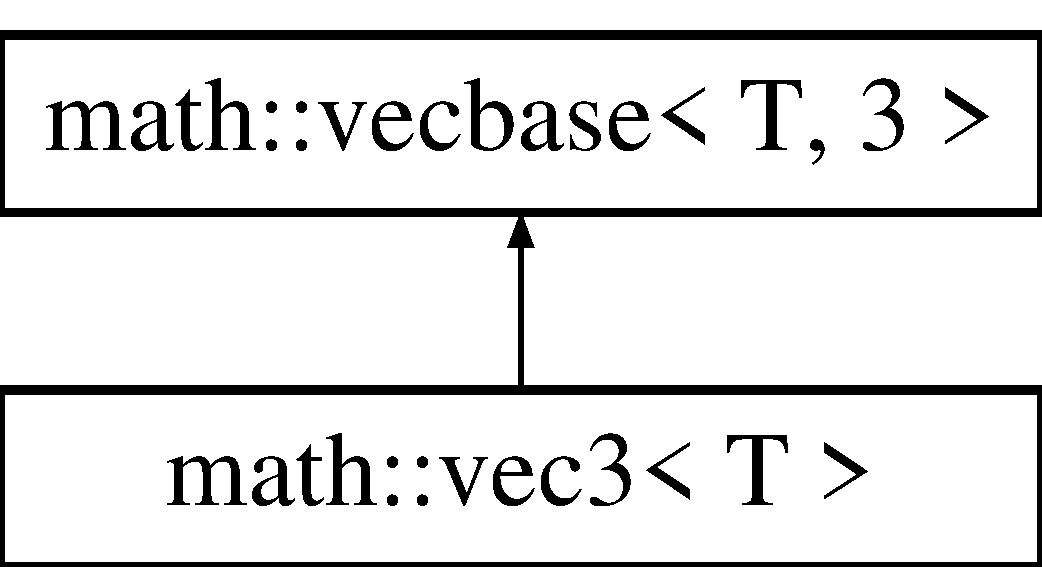
\includegraphics[height=2cm]{classmath_1_1vec3}
\end{center}
\end{figure}
\subsection*{Public Member Functions}
\begin{DoxyCompactItemize}
\item 
\hypertarget{classmath_1_1vec3_aefe52aac96775f53d657791022048657}{
double {\bfseries dot} (\hyperlink{classmath_1_1vec3}{math::vec3}$<$ T $>$ const \&rhs) const }
\label{classmath_1_1vec3_aefe52aac96775f53d657791022048657}

\item 
\hypertarget{classmath_1_1vec3_a3690718d39b1e8f0a8343137b23c4cfe}{
\hyperlink{classmath_1_1vec3}{math::vec3}$<$ T $>$ {\bfseries cross} (const \hyperlink{classmath_1_1vec3}{vec3}$<$ T $>$ \&rhs) const }
\label{classmath_1_1vec3_a3690718d39b1e8f0a8343137b23c4cfe}

\item 
\hypertarget{classmath_1_1vec3_a57e9cdf743e97f6256aa72af644c3543}{
T {\bfseries angle} (\hyperlink{classmath_1_1vec3}{vec3}$<$ T $>$ const \&rhs) const }
\label{classmath_1_1vec3_a57e9cdf743e97f6256aa72af644c3543}

\item 
\hypertarget{classmath_1_1vec3_ad943b48e270a599e86a8438c74b982ec}{
\hyperlink{classmath_1_1vec3}{math::vec3}$<$ T $>$ {\bfseries GetNormalized} () const }
\label{classmath_1_1vec3_ad943b48e270a599e86a8438c74b982ec}

\item 
\hypertarget{classmath_1_1vec3_ac8c3afa853d432be6057d19e7d80505d}{
\hyperlink{classmath_1_1vec3}{math::vec3}$<$ T $>$ {\bfseries GetRotatedX} (double angle) const }
\label{classmath_1_1vec3_ac8c3afa853d432be6057d19e7d80505d}

\item 
\hypertarget{classmath_1_1vec3_a3f44607ec66f38a42e357cedaff4838e}{
void {\bfseries RotateX} (double angle)}
\label{classmath_1_1vec3_a3f44607ec66f38a42e357cedaff4838e}

\item 
\hypertarget{classmath_1_1vec3_ac38729bb7d1a37203b805abe30b6aded}{
\hyperlink{classmath_1_1vec3}{math::vec3}$<$ T $>$ {\bfseries GetRotatedY} (double angle) const }
\label{classmath_1_1vec3_ac38729bb7d1a37203b805abe30b6aded}

\item 
\hypertarget{classmath_1_1vec3_a2da382572748410a8b83b5a5cb81779f}{
void {\bfseries RotateY} (double angle)}
\label{classmath_1_1vec3_a2da382572748410a8b83b5a5cb81779f}

\item 
\hypertarget{classmath_1_1vec3_acdf735154a892bc3483944ac8418b82a}{
\hyperlink{classmath_1_1vec3}{math::vec3}$<$ T $>$ {\bfseries GetRotatedZ} (double angle) const }
\label{classmath_1_1vec3_acdf735154a892bc3483944ac8418b82a}

\item 
\hypertarget{classmath_1_1vec3_aeebdb2765988f12467c2b5494595ccc5}{
void {\bfseries RotateZ} (double angle)}
\label{classmath_1_1vec3_aeebdb2765988f12467c2b5494595ccc5}

\item 
\hypertarget{classmath_1_1vec3_a1e32d34ba4af2ca4d3e93dd6089815a8}{
\hyperlink{classmath_1_1vec3}{math::vec3}$<$ T $>$ {\bfseries GetRotatedAxis} (double angle, const \hyperlink{classmath_1_1vec3}{math::vec3}$<$ T $>$ \&axis) const }
\label{classmath_1_1vec3_a1e32d34ba4af2ca4d3e93dd6089815a8}

\item 
\hypertarget{classmath_1_1vec3_a2834906e384cd12364a0cfc7aa633fd6}{
void {\bfseries PackTo01} ()}
\label{classmath_1_1vec3_a2834906e384cd12364a0cfc7aa633fd6}

\item 
\hypertarget{classmath_1_1vec3_a9e1747a7966f2673d07435825dfd7425}{
\hyperlink{classmath_1_1vec3}{math::vec3}$<$ T $>$ {\bfseries GetPackedTo01} () const }
\label{classmath_1_1vec3_a9e1747a7966f2673d07435825dfd7425}

\item 
\hypertarget{classmath_1_1vec3_ae60dea9bcf2b847d475ad640a7b8851b}{
\hyperlink{classmath_1_1vec3}{vec3}$<$ T $>$ {\bfseries lerp} (const \hyperlink{classmath_1_1vec3}{vec3}$<$ T $>$ \&v2, T factor) const }
\label{classmath_1_1vec3_ae60dea9bcf2b847d475ad640a7b8851b}

\item 
\hypertarget{classmath_1_1vec3_a105110ab02f529670bd32653f77e864a}{
\hyperlink{classmath_1_1vec3}{vec3}$<$ T $>$ {\bfseries QuadraticInterpolate} (const \hyperlink{classmath_1_1vec3}{vec3}$<$ T $>$ \&v2, const \hyperlink{classmath_1_1vec3}{vec3}$<$ T $>$ \&v3, T factor) const }
\label{classmath_1_1vec3_a105110ab02f529670bd32653f77e864a}

\item 
\hypertarget{classmath_1_1vec3_a9fff5b62a267357932db72711431aaec}{
\hyperlink{classmath_1_1vec3}{vec3}$<$ T $>$ {\bfseries operator-\/} () const }
\label{classmath_1_1vec3_a9fff5b62a267357932db72711431aaec}

\item 
\hypertarget{classmath_1_1vec3_a023dcce232314615765661050e4eb542}{
\hyperlink{classmath_1_1vec3}{vec3}$<$ T $>$ {\bfseries operator+} () const }
\label{classmath_1_1vec3_a023dcce232314615765661050e4eb542}

\item 
\hypertarget{classmath_1_1vec3_aba9492a415256e0c647bcc719b914430}{
\hyperlink{classmath_1_1vec3}{vec3}$<$ T $>$ {\bfseries Abs} ()}
\label{classmath_1_1vec3_aba9492a415256e0c647bcc719b914430}

\item 
\hypertarget{classmath_1_1vec3_acb820fcead5ddafeb6dde5bc52807b06}{
bool {\bfseries operator$<$} (\hyperlink{classmath_1_1vec3}{vec3}$<$ T $>$ const \&rhs)}
\label{classmath_1_1vec3_acb820fcead5ddafeb6dde5bc52807b06}

\item 
\hypertarget{classmath_1_1vec3_a5e4169f776dad4d3f3364ba0289321cb}{
{\bfseries operator T $\ast$} () const }
\label{classmath_1_1vec3_a5e4169f776dad4d3f3364ba0289321cb}

\item 
\hypertarget{classmath_1_1vec3_af5a8cf41a9216e6f52e2f0a105f17ee2}{
{\bfseries operator const T $\ast$} () const }
\label{classmath_1_1vec3_af5a8cf41a9216e6f52e2f0a105f17ee2}

\item 
\hypertarget{classmath_1_1vec3_a6b660d27a7bf07fe8b5ac19f0fc8b908}{
void {\bfseries RotateAxis} (double angle, const \hyperlink{classmath_1_1vec3}{math::vec3}$<$ T $>$ \&axis)}
\label{classmath_1_1vec3_a6b660d27a7bf07fe8b5ac19f0fc8b908}

\item 
\hypertarget{classmath_1_1vec3_a587e1d4e4ba254d049db04e1afb8773f}{
void {\bfseries print} () const }
\label{classmath_1_1vec3_a587e1d4e4ba254d049db04e1afb8773f}

\end{DoxyCompactItemize}
\begin{Indent}{\bf constructors}\par
{\em \label{_amgrp0d8243d493859cb6cbec161117e79b0d}
 }\begin{DoxyCompactItemize}
\item 
\hypertarget{classmath_1_1vec3_a1c9db4362d233790c6d8f4a896b77a3f}{
{\bfseries vec3} ()}
\label{classmath_1_1vec3_a1c9db4362d233790c6d8f4a896b77a3f}

\item 
\hypertarget{classmath_1_1vec3_a6faf6197cea623fc525e7b45fe7a5708}{
{\bfseries vec3} (\hyperlink{classmath_1_1vec3}{math::vec3}$<$ T $>$ const \&rhs)}
\label{classmath_1_1vec3_a6faf6197cea623fc525e7b45fe7a5708}

\item 
\hypertarget{classmath_1_1vec3_a6a8c24654f1cd0904bec64f5a96b9649}{
{\bfseries vec3} (double const \&nx, double const \&ny, double const \&nz)}
\label{classmath_1_1vec3_a6a8c24654f1cd0904bec64f5a96b9649}

\item 
\hypertarget{classmath_1_1vec3_a0aa664d081e6235be5a4d70245023a75}{
{\bfseries vec3} (double const $\ast$const v)}
\label{classmath_1_1vec3_a0aa664d081e6235be5a4d70245023a75}

\end{DoxyCompactItemize}
\end{Indent}
\begin{Indent}{\bf accessors}\par
{\em \label{_amgrp7c8b08feaff3919fb1a0d86dd0b50597}
 }\begin{DoxyCompactItemize}
\item 
\hypertarget{classmath_1_1vec3_a21cb93bfdb9a5e19dc86679660a4c828}{
T \& {\bfseries x} ()}
\label{classmath_1_1vec3_a21cb93bfdb9a5e19dc86679660a4c828}

\item 
\hypertarget{classmath_1_1vec3_ad8cd95e181b94881668195c0316a6487}{
T \& {\bfseries y} ()}
\label{classmath_1_1vec3_ad8cd95e181b94881668195c0316a6487}

\item 
\hypertarget{classmath_1_1vec3_a68619b85c6312c3a45a37da23583219b}{
T \& {\bfseries z} ()}
\label{classmath_1_1vec3_a68619b85c6312c3a45a37da23583219b}

\end{DoxyCompactItemize}
\end{Indent}
\begin{Indent}{\bf binary operators}\par
{\em \label{_amgrp04c8a55c25fdc9a3444da113de31256d}
 }\begin{DoxyCompactItemize}
\item 
\hypertarget{classmath_1_1vec3_adaf198c54d56f4bf4493b91919f6eb8e}{
\hyperlink{classmath_1_1vec3}{vec3}$<$ T $>$ {\bfseries operator+} (const \hyperlink{classmath_1_1vec3}{vec3}$<$ T $>$ \&rhs) const }
\label{classmath_1_1vec3_adaf198c54d56f4bf4493b91919f6eb8e}

\item 
\hypertarget{classmath_1_1vec3_ab79da731edca6736172a2ec4bc7a9be7}{
\hyperlink{classmath_1_1vec3}{vec3}$<$ T $>$ {\bfseries operator-\/} (const \hyperlink{classmath_1_1vec3}{vec3}$<$ T $>$ \&rhs) const }
\label{classmath_1_1vec3_ab79da731edca6736172a2ec4bc7a9be7}

\item 
\hypertarget{classmath_1_1vec3_a0158485443f1a333c17d68f48ec1534b}{
\hyperlink{classmath_1_1vec3}{vec3}$<$ T $>$ {\bfseries operator$\ast$} (const double rhs) const }
\label{classmath_1_1vec3_a0158485443f1a333c17d68f48ec1534b}

\item 
\hypertarget{classmath_1_1vec3_afb842d06e9ee3d446c01b16ed870f20b}{
\hyperlink{classmath_1_1vec3}{vec3}$<$ T $>$ {\bfseries operator/} (const double rhs) const }
\label{classmath_1_1vec3_afb842d06e9ee3d446c01b16ed870f20b}

\item 
\hypertarget{classmath_1_1vec3_ab0578e01e8adbea1568501ce11170ba1}{
void {\bfseries Add} (const \hyperlink{classmath_1_1vec3}{vec3}$<$ T $>$ \&v2, \hyperlink{classmath_1_1vec3}{vec3}$<$ T $>$ \&result)}
\label{classmath_1_1vec3_ab0578e01e8adbea1568501ce11170ba1}

\item 
\hypertarget{classmath_1_1vec3_a768ea8bebdeb56697afe8446e551549c}{
void {\bfseries Subtract} (const \hyperlink{classmath_1_1vec3}{vec3}$<$ T $>$ \&v2, \hyperlink{classmath_1_1vec3}{vec3}$<$ T $>$ \&result)}
\label{classmath_1_1vec3_a768ea8bebdeb56697afe8446e551549c}

\end{DoxyCompactItemize}
\end{Indent}
\begin{Indent}{\bf comparison}\par
{\em \label{_amgrp347cd68a17ba31d02e83262794a3c9e3}
 }\begin{DoxyCompactItemize}
\item 
\hypertarget{classmath_1_1vec3_a2f2dfd6ab85413e1e6cb890eac45a0ab}{
bool {\bfseries operator==} (const \hyperlink{classmath_1_1vec3}{math::vec3}$<$ T $>$ \&rhs) const }
\label{classmath_1_1vec3_a2f2dfd6ab85413e1e6cb890eac45a0ab}

\item 
\hypertarget{classmath_1_1vec3_a826506266eb9749d197e1fcaf2a84904}{
bool {\bfseries operator!=} (const \hyperlink{classmath_1_1vec3}{vec3}$<$ T $>$ \&rhs) const }
\label{classmath_1_1vec3_a826506266eb9749d197e1fcaf2a84904}

\end{DoxyCompactItemize}
\end{Indent}
\begin{Indent}{\bf self operators}\par
{\em \label{_amgrpf8b7a2ea730234c9f4b728de7bf6a056}
 }\begin{DoxyCompactItemize}
\item 
\hypertarget{classmath_1_1vec3_a04f6aee5e3b4bcf9283b844bd279b399}{
\hyperlink{classmath_1_1vec3}{math::vec3}$<$ T $>$ \& {\bfseries operator+=} (\hyperlink{classmath_1_1vec3}{math::vec3}$<$ T $>$ const \&rhs)}
\label{classmath_1_1vec3_a04f6aee5e3b4bcf9283b844bd279b399}

\item 
\hypertarget{classmath_1_1vec3_ad46ac632fb51c7dbcd0bf92bff1da878}{
\hyperlink{classmath_1_1vec3}{math::vec3}$<$ T $>$ \& {\bfseries operator-\/=} (const \hyperlink{classmath_1_1vec3}{vec3}$<$ T $>$ \&rhs)}
\label{classmath_1_1vec3_ad46ac632fb51c7dbcd0bf92bff1da878}

\item 
\hypertarget{classmath_1_1vec3_a816296f3311ad6124f7f210a047ca9a7}{
\hyperlink{classmath_1_1vec3}{math::vec3}$<$ T $>$ \& {\bfseries operator$\ast$=} (const double rhs)}
\label{classmath_1_1vec3_a816296f3311ad6124f7f210a047ca9a7}

\item 
\hypertarget{classmath_1_1vec3_ae189ca8cec1e6548d3603e81addeeda3}{
\hyperlink{classmath_1_1vec3}{math::vec3}$<$ T $>$ \& {\bfseries operator/=} (const double rhs)}
\label{classmath_1_1vec3_ae189ca8cec1e6548d3603e81addeeda3}

\end{DoxyCompactItemize}
\end{Indent}
\subsubsection*{template$<$typename T$>$ class math::vec3$<$ T $>$}



The documentation for this class was generated from the following file:\begin{DoxyCompactItemize}
\item 
src/math/vec3.h\end{DoxyCompactItemize}

\hypertarget{classmath_1_1vec4}{
\section{math::vec4$<$ T $>$ Class Template Reference}
\label{classmath_1_1vec4}\index{math::vec4@{math::vec4}}
}
Inheritance diagram for math::vec4$<$ T $>$::\begin{figure}[H]
\begin{center}
\leavevmode
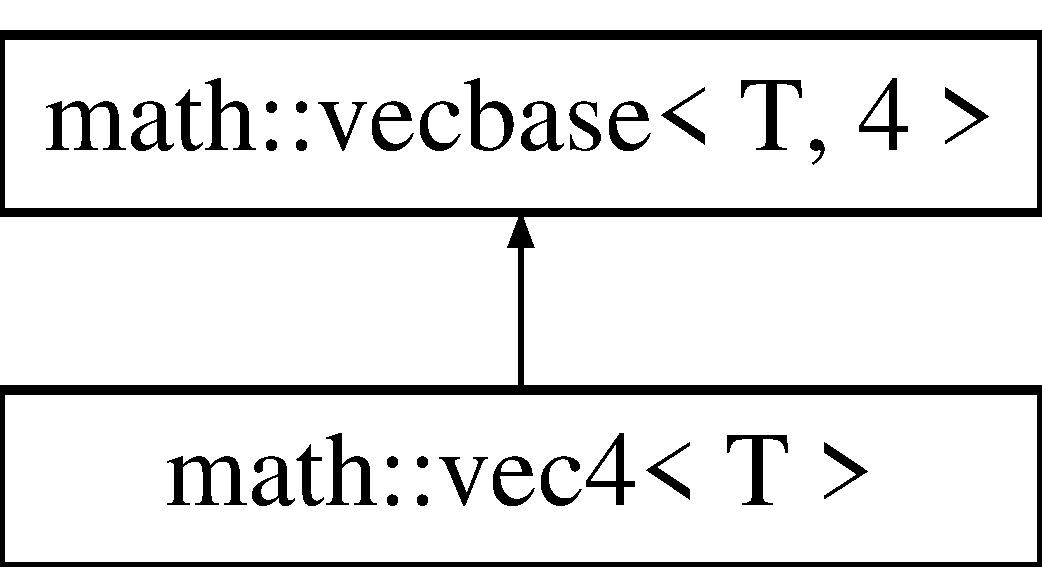
\includegraphics[height=2cm]{classmath_1_1vec4}
\end{center}
\end{figure}
\subsection*{Public Member Functions}
\begin{DoxyCompactItemize}
\item 
\hypertarget{classmath_1_1vec4_ae29babb2f7feddd0682cee16e2e7423c}{
T \& {\bfseries w} ()}
\label{classmath_1_1vec4_ae29babb2f7feddd0682cee16e2e7423c}

\item 
\hypertarget{classmath_1_1vec4_adb62edeee673cf471c4f80ca82ca2995}{
T \& {\bfseries x} ()}
\label{classmath_1_1vec4_adb62edeee673cf471c4f80ca82ca2995}

\item 
\hypertarget{classmath_1_1vec4_af24ce6557df36a22ee17946a8cb3ef67}{
T \& {\bfseries y} ()}
\label{classmath_1_1vec4_af24ce6557df36a22ee17946a8cb3ef67}

\item 
\hypertarget{classmath_1_1vec4_a15af37a2f72c15ea777516eb9ced43e7}{
T \& {\bfseries z} ()}
\label{classmath_1_1vec4_a15af37a2f72c15ea777516eb9ced43e7}

\item 
\hypertarget{classmath_1_1vec4_a3f14cbf091c8f58973f978b55a2744d5}{
{\bfseries operator math::vec3$<$ T $>$} ()}
\label{classmath_1_1vec4_a3f14cbf091c8f58973f978b55a2744d5}

\item 
\hypertarget{classmath_1_1vec4_a997a5c8cf9080ce670644ba9a1454407}{
\hyperlink{classmath_1_1mat44}{math::mat44}$<$ T $>$ {\bfseries operator$\ast$} (\hyperlink{classmath_1_1vec4}{math::vec4}$<$ T $>$ const \&rhs)}
\label{classmath_1_1vec4_a997a5c8cf9080ce670644ba9a1454407}

\item 
\hypertarget{classmath_1_1vec4_a48e9b9e91a4ff955973b346b957337c6}{
void {\bfseries print} ()}
\label{classmath_1_1vec4_a48e9b9e91a4ff955973b346b957337c6}

\item 
\hypertarget{classmath_1_1vec4_a455ee3b682ee0036a90794b1235ec615}{
void {\bfseries Set} (T newX, T newY, T newZ, T newW)}
\label{classmath_1_1vec4_a455ee3b682ee0036a90794b1235ec615}

\item 
\hypertarget{classmath_1_1vec4_a59f1ffa6b8218c9568afd841bef85825}{
void {\bfseries SetX} (T newX)}
\label{classmath_1_1vec4_a59f1ffa6b8218c9568afd841bef85825}

\item 
\hypertarget{classmath_1_1vec4_ab5a1f413c86ede41967ada2b72059685}{
void {\bfseries SetY} (T newY)}
\label{classmath_1_1vec4_ab5a1f413c86ede41967ada2b72059685}

\item 
\hypertarget{classmath_1_1vec4_ab6b16d41d26526c301c319ef3d724c94}{
void {\bfseries SetZ} (T newZ)}
\label{classmath_1_1vec4_ab6b16d41d26526c301c319ef3d724c94}

\item 
\hypertarget{classmath_1_1vec4_aab15f29bbc9e07e2a788c0fd2399c97f}{
void {\bfseries SetW} (T newW)}
\label{classmath_1_1vec4_aab15f29bbc9e07e2a788c0fd2399c97f}

\item 
\hypertarget{classmath_1_1vec4_a996db2662ab13120350ef3234618d921}{
T {\bfseries GetX} () const }
\label{classmath_1_1vec4_a996db2662ab13120350ef3234618d921}

\item 
\hypertarget{classmath_1_1vec4_ac06c44a0e840bde6171fb2f18461d5a2}{
T {\bfseries GetY} () const }
\label{classmath_1_1vec4_ac06c44a0e840bde6171fb2f18461d5a2}

\item 
\hypertarget{classmath_1_1vec4_af03172026b89f7b514d05eadd5d33360}{
T {\bfseries GetZ} () const }
\label{classmath_1_1vec4_af03172026b89f7b514d05eadd5d33360}

\item 
\hypertarget{classmath_1_1vec4_a37c74aff9f93d229c5218ad57b20bc69}{
T {\bfseries GetW} () const }
\label{classmath_1_1vec4_a37c74aff9f93d229c5218ad57b20bc69}

\item 
\hypertarget{classmath_1_1vec4_a89f5cbcdaebeba00e49ca3ad48b50e54}{
void {\bfseries LoadZero} (void)}
\label{classmath_1_1vec4_a89f5cbcdaebeba00e49ca3ad48b50e54}

\item 
\hypertarget{classmath_1_1vec4_af2ef943623b385a1f93d7369005c18b6}{
void {\bfseries LoadOne} (void)}
\label{classmath_1_1vec4_af2ef943623b385a1f93d7369005c18b6}

\item 
\hypertarget{classmath_1_1vec4_a3716bb581ac654c528edd07dd34f7ba3}{
T {\bfseries dot} (const \hyperlink{classmath_1_1vec4}{vec4} \&rhs)}
\label{classmath_1_1vec4_a3716bb581ac654c528edd07dd34f7ba3}

\item 
\hypertarget{classmath_1_1vec4_ae035ab0de6e786e8c30fb547eb222769}{
\hyperlink{classmath_1_1vec4}{vec4} {\bfseries lerp} (const \hyperlink{classmath_1_1vec4}{vec4} \&v2, T factor) const }
\label{classmath_1_1vec4_ae035ab0de6e786e8c30fb547eb222769}

\item 
\hypertarget{classmath_1_1vec4_af2da5bdd1816c17598525f9003bcb38a}{
\hyperlink{classmath_1_1vec4}{vec4} {\bfseries QuadraticInterpolate} (const \hyperlink{classmath_1_1vec4}{vec4} \&v2, const \hyperlink{classmath_1_1vec4}{vec4} \&v3, T factor) const }
\label{classmath_1_1vec4_af2da5bdd1816c17598525f9003bcb38a}

\item 
\hypertarget{classmath_1_1vec4_a8c33ef79e16b829a103bf0cbc16a8a67}{
\hyperlink{classmath_1_1vec4}{vec4} {\bfseries operator+} (const \hyperlink{classmath_1_1vec4}{vec4} \&rhs) const }
\label{classmath_1_1vec4_a8c33ef79e16b829a103bf0cbc16a8a67}

\item 
\hypertarget{classmath_1_1vec4_af18d39639101dfb6085e6203286ba73a}{
\hyperlink{classmath_1_1vec4}{vec4} {\bfseries operator+} (const T \&rhs) const }
\label{classmath_1_1vec4_af18d39639101dfb6085e6203286ba73a}

\item 
\hypertarget{classmath_1_1vec4_accff5e11b577e3e346582ae11344ad8a}{
\hyperlink{classmath_1_1vec4}{vec4} {\bfseries operator-\/} (const \hyperlink{classmath_1_1vec4}{vec4} \&rhs) const }
\label{classmath_1_1vec4_accff5e11b577e3e346582ae11344ad8a}

\item 
\hypertarget{classmath_1_1vec4_a670a6ac60b4212efc3de4406df80a3ad}{
\hyperlink{classmath_1_1vec4}{vec4} {\bfseries operator$\ast$} (const T rhs) const }
\label{classmath_1_1vec4_a670a6ac60b4212efc3de4406df80a3ad}

\item 
\hypertarget{classmath_1_1vec4_a27a6fd77499f76c6929aaffedd09632f}{
\hyperlink{classmath_1_1vec4}{vec4} {\bfseries operator/} (const T rhs) const }
\label{classmath_1_1vec4_a27a6fd77499f76c6929aaffedd09632f}

\item 
\hypertarget{classmath_1_1vec4_a9540a2d6ad687fbd4e6bf2b16abbcfa7}{
void {\bfseries operator+=} (const \hyperlink{classmath_1_1vec4}{vec4} \&rhs)}
\label{classmath_1_1vec4_a9540a2d6ad687fbd4e6bf2b16abbcfa7}

\item 
\hypertarget{classmath_1_1vec4_a13e0880525d0078e945e5f35c2b276c0}{
void {\bfseries operator-\/=} (const \hyperlink{classmath_1_1vec4}{vec4} \&rhs)}
\label{classmath_1_1vec4_a13e0880525d0078e945e5f35c2b276c0}

\item 
\hypertarget{classmath_1_1vec4_a6490ec9ed4da3a50b168f945d0bcbb7b}{
void {\bfseries operator$\ast$=} (const T rhs)}
\label{classmath_1_1vec4_a6490ec9ed4da3a50b168f945d0bcbb7b}

\item 
\hypertarget{classmath_1_1vec4_a20518d8b8880dfb435bb443819a1e0bc}{
void {\bfseries operator/=} (const T rhs)}
\label{classmath_1_1vec4_a20518d8b8880dfb435bb443819a1e0bc}

\item 
\hypertarget{classmath_1_1vec4_a7262663b102b2d44c8aa686ed90e33ad}{
{\bfseries operator T $\ast$} () const }
\label{classmath_1_1vec4_a7262663b102b2d44c8aa686ed90e33ad}

\item 
\hypertarget{classmath_1_1vec4_a96dba80b67fb27aafd0dbf23070bb5e4}{
{\bfseries operator const T $\ast$} () const }
\label{classmath_1_1vec4_a96dba80b67fb27aafd0dbf23070bb5e4}

\end{DoxyCompactItemize}
\begin{Indent}{\bf Constructors}\par
{\em \label{_amgrp559a25fdb98a7d1fd1c3771ac568d5e9}
 }\begin{DoxyCompactItemize}
\item 
\hypertarget{classmath_1_1vec4_a8a5e9324ce00792995883c2b1668ba3a}{
{\bfseries vec4} (const \hyperlink{classmath_1_1vec3}{vec3}$<$ T $>$ \&rhs)}
\label{classmath_1_1vec4_a8a5e9324ce00792995883c2b1668ba3a}

\item 
\hypertarget{classmath_1_1vec4_a1854eb9c26e3451471ccc5f204e05f94}{
{\bfseries vec4} (\hyperlink{classmath_1_1vec3}{vec3}$<$ T $>$ const \&rhs, T const \&newW)}
\label{classmath_1_1vec4_a1854eb9c26e3451471ccc5f204e05f94}

\item 
\hypertarget{classmath_1_1vec4_acd70cfec2ef8ac46c9756b4044beecaa}{
{\bfseries vec4} ()}
\label{classmath_1_1vec4_acd70cfec2ef8ac46c9756b4044beecaa}

\item 
\hypertarget{classmath_1_1vec4_aa5fcadd0ce581569e82ee0b14e7a4cc0}{
{\bfseries vec4} (T newX, T newY, T newZ, T newW)}
\label{classmath_1_1vec4_aa5fcadd0ce581569e82ee0b14e7a4cc0}

\item 
\hypertarget{classmath_1_1vec4_ab970028d7608787f3e6ca0eb6ce14669}{
{\bfseries vec4} (T const $\ast$rhs)}
\label{classmath_1_1vec4_ab970028d7608787f3e6ca0eb6ce14669}

\item 
\hypertarget{classmath_1_1vec4_a0e5fa5f584295fe1b6bb66ebcbcb01e9}{
{\bfseries vec4} (const \hyperlink{classmath_1_1vec4}{vec4} \&rhs)}
\label{classmath_1_1vec4_a0e5fa5f584295fe1b6bb66ebcbcb01e9}

\end{DoxyCompactItemize}
\end{Indent}
\begin{Indent}{\bf Rotations}\par
{\em \label{_amgrpe3a9f3ceea2a861d915023ad0a1b98b0}
 }\begin{DoxyCompactItemize}
\item 
\hypertarget{classmath_1_1vec4_a0c0b102f730831e00f43a23a1561bbf1}{
void {\bfseries rotateX} (T angle)}
\label{classmath_1_1vec4_a0c0b102f730831e00f43a23a1561bbf1}

\item 
\hypertarget{classmath_1_1vec4_a7fd5f6afb20d428b36ce25725258018c}{
\hyperlink{classmath_1_1vec4}{vec4}$<$ T $>$ {\bfseries getRotatedX} (T angle) const }
\label{classmath_1_1vec4_a7fd5f6afb20d428b36ce25725258018c}

\item 
\hypertarget{classmath_1_1vec4_a0e143a0a52e0a8a0d4e0f08e588cda84}{
void {\bfseries rotateY} (T angle)}
\label{classmath_1_1vec4_a0e143a0a52e0a8a0d4e0f08e588cda84}

\item 
\hypertarget{classmath_1_1vec4_a601aac1fa9439d44fe52fe0b49c185b7}{
\hyperlink{classmath_1_1vec4}{vec4}$<$ T $>$ {\bfseries getRotatedY} (T angle) const }
\label{classmath_1_1vec4_a601aac1fa9439d44fe52fe0b49c185b7}

\item 
\hypertarget{classmath_1_1vec4_a18d44d4896f3d93d960f5eddb7618c07}{
void {\bfseries rotateZ} (T angle)}
\label{classmath_1_1vec4_a18d44d4896f3d93d960f5eddb7618c07}

\item 
\hypertarget{classmath_1_1vec4_adc8bbf0a6e2ea9948d2d6d9af6f3d2d2}{
\hyperlink{classmath_1_1vec4}{vec4}$<$ T $>$ {\bfseries getRotatedZ} (T angle) const }
\label{classmath_1_1vec4_adc8bbf0a6e2ea9948d2d6d9af6f3d2d2}

\item 
\hypertarget{classmath_1_1vec4_a36713f548216b66841ba0598ee6d71d4}{
void {\bfseries rotateAxis} (T angle, const \hyperlink{classmath_1_1vec3}{math::vec3}$<$ T $>$ \&axis)}
\label{classmath_1_1vec4_a36713f548216b66841ba0598ee6d71d4}

\item 
\hypertarget{classmath_1_1vec4_ad0e8c7e272108fa16a95db2a5537936d}{
\hyperlink{classmath_1_1vec4}{math::vec4}$<$ T $>$ {\bfseries getRotatedAxis} (T angle, const \hyperlink{classmath_1_1vec3}{math::vec3}$<$ T $>$ \&axis) const }
\label{classmath_1_1vec4_ad0e8c7e272108fa16a95db2a5537936d}

\end{DoxyCompactItemize}
\end{Indent}
\begin{Indent}{\bf Comparison}\par
{\em \label{_amgrpf6c0e3a1c3cfabd32ae8d3ae741fcf0a}
 }\begin{DoxyCompactItemize}
\item 
\hypertarget{classmath_1_1vec4_a2b7541c1d4dfed7029c867b3f1439b50}{
bool {\bfseries operator==} (const \hyperlink{classmath_1_1vec4}{math::vec4}$<$ T $>$ \&rhs) const }
\label{classmath_1_1vec4_a2b7541c1d4dfed7029c867b3f1439b50}

\item 
\hypertarget{classmath_1_1vec4_a6a4dfdb631aa3c8879740d2be4872285}{
bool {\bfseries operator!=} (const \hyperlink{classmath_1_1vec4}{vec4} \&rhs) const }
\label{classmath_1_1vec4_a6a4dfdb631aa3c8879740d2be4872285}

\end{DoxyCompactItemize}
\end{Indent}
\subsubsection*{template$<$typename T$>$ class math::vec4$<$ T $>$}



The documentation for this class was generated from the following file:\begin{DoxyCompactItemize}
\item 
src/math/vec4.hpp\end{DoxyCompactItemize}

\hypertarget{classmath_1_1vecbase}{
\section{math::vecbase$<$ T, N $>$ Class Template Reference}
\label{classmath_1_1vecbase}\index{math::vecbase@{math::vecbase}}
}
Inheritance diagram for math::vecbase$<$ T, N $>$::\begin{figure}[H]
\begin{center}
\leavevmode
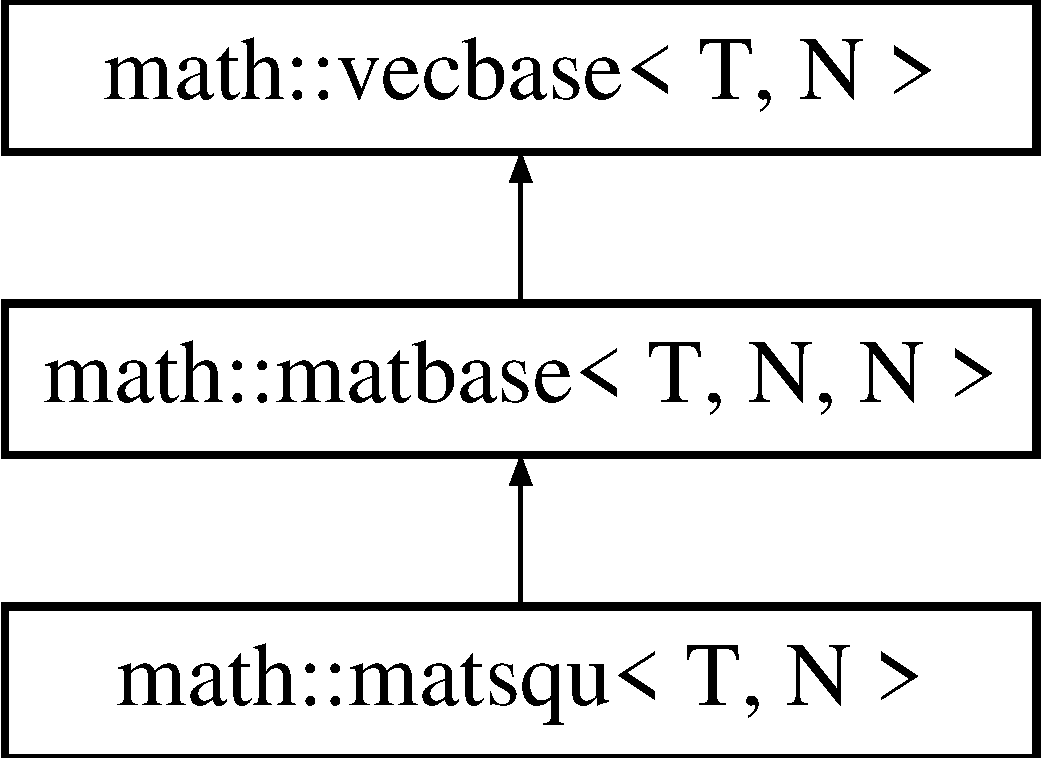
\includegraphics[height=3cm]{classmath_1_1vecbase}
\end{center}
\end{figure}
\subsection*{Public Types}
\begin{DoxyCompactItemize}
\item 
\hypertarget{classmath_1_1vecbase_a26c60dd255fe154d21df8d22d4e97e10}{
typedef T {\bfseries Type}}
\label{classmath_1_1vecbase_a26c60dd255fe154d21df8d22d4e97e10}

\end{DoxyCompactItemize}
\subsection*{Public Member Functions}
\begin{DoxyCompactItemize}
\item 
\hypertarget{classmath_1_1vecbase_ace789b2c8321e0d058b5cd143df2e439}{
{\bfseries vecbase} (T const $\ast$const rhs)}
\label{classmath_1_1vecbase_ace789b2c8321e0d058b5cd143df2e439}

\item 
\hypertarget{classmath_1_1vecbase_a79960000898a0987a7579fc40fca4bbd}{
void {\bfseries LoadZero} ()}
\label{classmath_1_1vecbase_a79960000898a0987a7579fc40fca4bbd}

\item 
\hypertarget{classmath_1_1vecbase_ac8e12f447b29967af11fb9f830fa08c2}{
double {\bfseries magnitude} () const }
\label{classmath_1_1vecbase_ac8e12f447b29967af11fb9f830fa08c2}

\item 
\hypertarget{classmath_1_1vecbase_ab620e8c531da5d6c86634fcb108646c1}{
void {\bfseries Normalize} ()}
\label{classmath_1_1vecbase_ab620e8c531da5d6c86634fcb108646c1}

\item 
\hypertarget{classmath_1_1vecbase_a7875c870c844f42aeaca952016a04bc7}{
bool {\bfseries IsFinite} () const }
\label{classmath_1_1vecbase_a7875c870c844f42aeaca952016a04bc7}

\item 
\hypertarget{classmath_1_1vecbase_a74f465a86765df211b97c716bc7162dc}{
bool {\bfseries IsNan} () const }
\label{classmath_1_1vecbase_a74f465a86765df211b97c716bc7162dc}

\item 
\hypertarget{classmath_1_1vecbase_a754b07a9163ae8746053ed8ca51e89c6}{
void {\bfseries write} (FILE $\ast$file) const }
\label{classmath_1_1vecbase_a754b07a9163ae8746053ed8ca51e89c6}

\item 
\hypertarget{classmath_1_1vecbase_a9759523e7304173f8ae57f3a9a30b37a}{
void {\bfseries read} (FILE $\ast$file)}
\label{classmath_1_1vecbase_a9759523e7304173f8ae57f3a9a30b37a}

\item 
\hypertarget{classmath_1_1vecbase_a80d2a8df6f5e4a6647531c98eb8fe595}{
T \& {\bfseries operator\mbox{[}$\,$\mbox{]}} (int i)}
\label{classmath_1_1vecbase_a80d2a8df6f5e4a6647531c98eb8fe595}

\end{DoxyCompactItemize}
\begin{Indent}{\bf vector algebra}\par
{\em \label{_amgrpf3df6783d0cca6c1ea518af64ed4d647}
 }\begin{DoxyCompactItemize}
\item 
\hypertarget{classmath_1_1vecbase_ae601a61c36ab5596610932ebe2f99f45}{
T {\bfseries dot} (\hyperlink{classmath_1_1vecbase}{vecbase}$<$ T, N $>$ const \&rhs)}
\label{classmath_1_1vecbase_ae601a61c36ab5596610932ebe2f99f45}

\end{DoxyCompactItemize}
\end{Indent}
\begin{Indent}{\bf binary operators}\par
{\em \label{_amgrp04c8a55c25fdc9a3444da113de31256d}
 }\begin{DoxyCompactItemize}
\item 
\hypertarget{classmath_1_1vecbase_aacfba6fee34bc6dfd105d955f675c74e}{
\hyperlink{classmath_1_1vecbase}{vecbase}$<$ T, N $>$ \& {\bfseries operator+=} (const \hyperlink{classmath_1_1vecbase}{vecbase}$<$ T, N $>$ \&rhs)}
\label{classmath_1_1vecbase_aacfba6fee34bc6dfd105d955f675c74e}

\item 
\hypertarget{classmath_1_1vecbase_a874c46c228e890efcbaa703b3a86b8f7}{
\hyperlink{classmath_1_1vecbase}{vecbase}$<$ T, N $>$ \& {\bfseries operator-\/=} (const \hyperlink{classmath_1_1vecbase}{vecbase}$<$ T, N $>$ \&rhs)}
\label{classmath_1_1vecbase_a874c46c228e890efcbaa703b3a86b8f7}

\item 
\hypertarget{classmath_1_1vecbase_a7a51537768ff2cde8b0a31fec39dee56}{
\hyperlink{classmath_1_1vecbase}{vecbase}$<$ T, N $>$ {\bfseries operator$\ast$=} (const double rhs)}
\label{classmath_1_1vecbase_a7a51537768ff2cde8b0a31fec39dee56}

\item 
\hypertarget{classmath_1_1vecbase_a06d655b27d88c726a2f5e9f100bc5e6a}{
\hyperlink{classmath_1_1vecbase}{vecbase}$<$ T, N $>$ {\bfseries operator/=} (const double rhs)}
\label{classmath_1_1vecbase_a06d655b27d88c726a2f5e9f100bc5e6a}

\end{DoxyCompactItemize}
\end{Indent}
\begin{Indent}{\bf unary operators}\par
{\em \label{_amgrp8839b6fa346915e1b72680f650c9b984}
 }\begin{DoxyCompactItemize}
\item 
\hypertarget{classmath_1_1vecbase_af814a8cd89b21afa5a0a156e2bb3bf72}{
\hyperlink{classmath_1_1vecbase}{vecbase}$<$ T, N $>$ \& {\bfseries minus} () const }
\label{classmath_1_1vecbase_af814a8cd89b21afa5a0a156e2bb3bf72}

\item 
\hypertarget{classmath_1_1vecbase_a0a02cdaf7cbaf2c454a8e124312bed5e}{
\hyperlink{classmath_1_1vecbase}{vecbase}$<$ T, N $>$ \& {\bfseries abs} ()}
\label{classmath_1_1vecbase_a0a02cdaf7cbaf2c454a8e124312bed5e}

\end{DoxyCompactItemize}
\end{Indent}
\subsection*{Public Attributes}
\begin{DoxyCompactItemize}
\item 
\hypertarget{classmath_1_1vecbase_ae357ff0254aaa64c7e72a93c64726d4c}{
T {\bfseries v} \mbox{[}N\mbox{]}}
\label{classmath_1_1vecbase_ae357ff0254aaa64c7e72a93c64726d4c}

\end{DoxyCompactItemize}
\subsection*{Protected Member Functions}
\begin{DoxyCompactItemize}
\item 
\hypertarget{classmath_1_1vecbase_a277e440413457a2a9431d53cd7eee3e3}{
bool {\bfseries operator$<$} (\hyperlink{classmath_1_1vecbase}{vecbase}$<$ T, N $>$ const \&rhs)}
\label{classmath_1_1vecbase_a277e440413457a2a9431d53cd7eee3e3}

\end{DoxyCompactItemize}
\subsubsection*{template$<$typename T, int N$>$ class math::vecbase$<$ T, N $>$}



The documentation for this class was generated from the following file:\begin{DoxyCompactItemize}
\item 
src/math/vecbase.h\end{DoxyCompactItemize}

\hypertarget{classvertex}{
\section{vertex Class Reference}
\label{classvertex}\index{vertex@{vertex}}
}
Inheritance diagram for vertex::\begin{figure}[H]
\begin{center}
\leavevmode
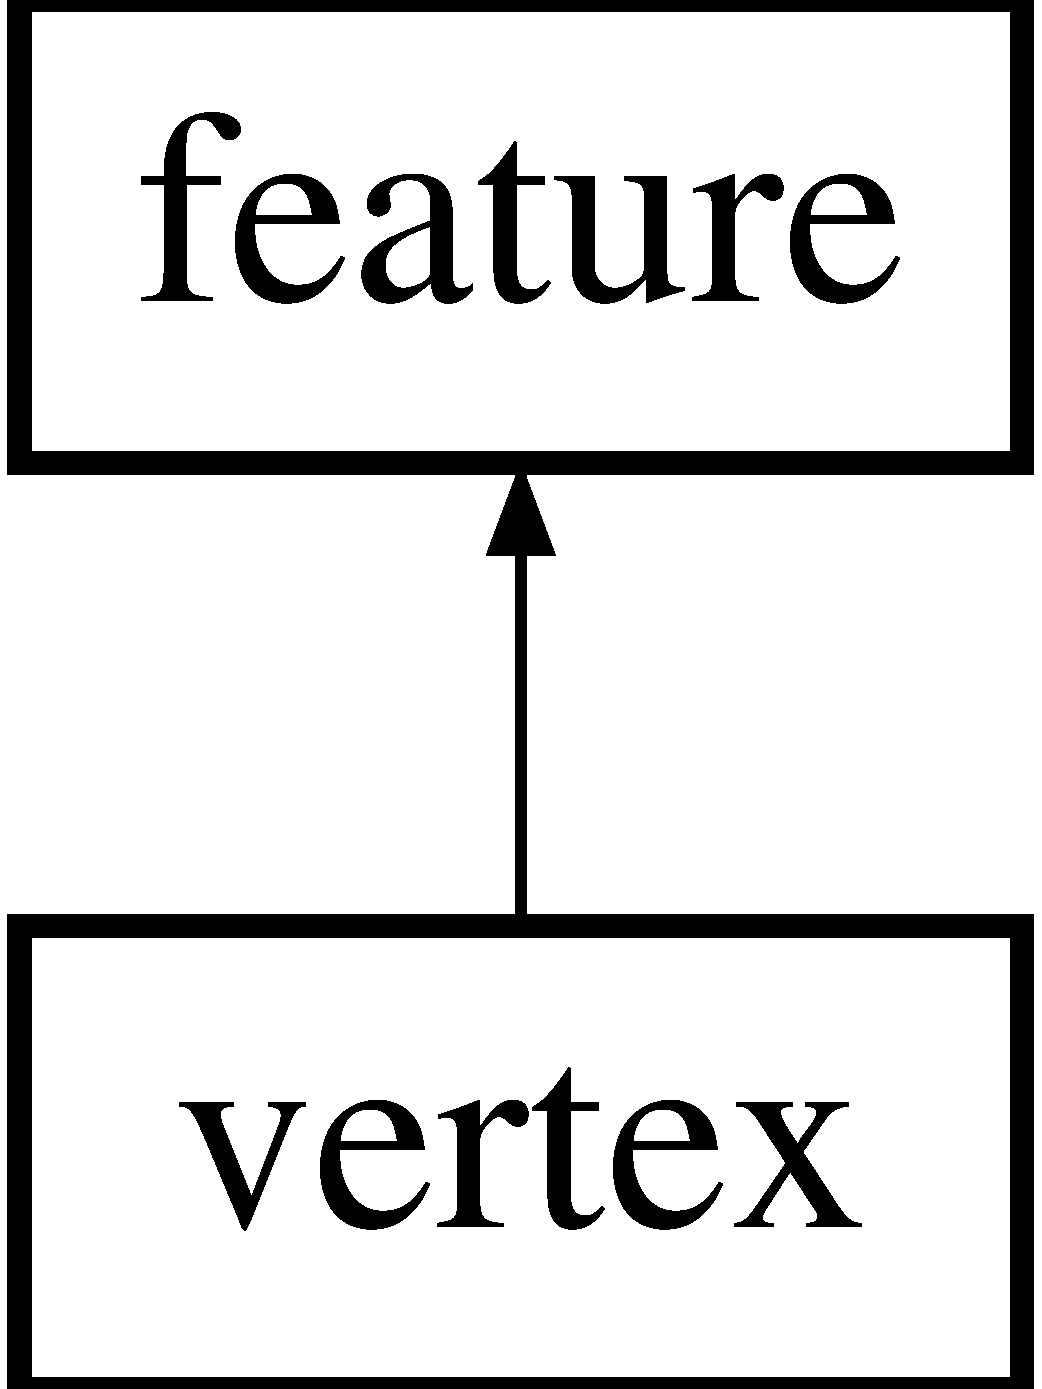
\includegraphics[height=2cm]{classvertex}
\end{center}
\end{figure}
\subsection*{Public Attributes}
\begin{DoxyCompactItemize}
\item 
\hypertarget{classvertex_a0cfa1be3d73ef4d1cd4a546f6c4b9b5d}{
std::set$<$ \hyperlink{classfeature}{feature} $\ast$ $>$ {\bfseries e}}
\label{classvertex_a0cfa1be3d73ef4d1cd4a546f6c4b9b5d}

\item 
\hypertarget{classvertex_a2981aef6dcfdc1f9cc3db752c4c3cfa2}{
\hyperlink{classmath_1_1vec3}{math::vec3}$<$ double $>$ {\bfseries v}}
\label{classvertex_a2981aef6dcfdc1f9cc3db752c4c3cfa2}

\end{DoxyCompactItemize}


The documentation for this class was generated from the following file:\begin{DoxyCompactItemize}
\item 
src/math/vclip/vclip.hpp\end{DoxyCompactItemize}

\hypertarget{classmath_1_1geo_1_1vertex}{
\section{math::geo::vertex Class Reference}
\label{classmath_1_1geo_1_1vertex}\index{math::geo::vertex@{math::geo::vertex}}
}
\subsection*{Public Attributes}
\begin{DoxyCompactItemize}
\item 
\hypertarget{classmath_1_1geo_1_1vertex_a3cfea2f74fcc452adb1adf0ffdb2ca7f}{
\hyperlink{classmath_1_1vec3}{vec3}$<$ double $>$ {\bfseries xyz}}
\label{classmath_1_1geo_1_1vertex_a3cfea2f74fcc452adb1adf0ffdb2ca7f}

\item 
\hypertarget{classmath_1_1geo_1_1vertex_ad89b7cb642fbf1332c05cd2534d02475}{
\hyperlink{classmath_1_1vec3}{vec3}$<$ double $>$ {\bfseries n}}
\label{classmath_1_1geo_1_1vertex_ad89b7cb642fbf1332c05cd2534d02475}

\end{DoxyCompactItemize}


The documentation for this class was generated from the following file:\begin{DoxyCompactItemize}
\item 
src/math/geo/polyhedron.hpp\end{DoxyCompactItemize}

\hypertarget{classmath_1_1geo_1_1wedge}{
\section{math::geo::wedge Class Reference}
\label{classmath_1_1geo_1_1wedge}\index{math::geo::wedge@{math::geo::wedge}}
}
Inheritance diagram for math::geo::wedge::\begin{figure}[H]
\begin{center}
\leavevmode
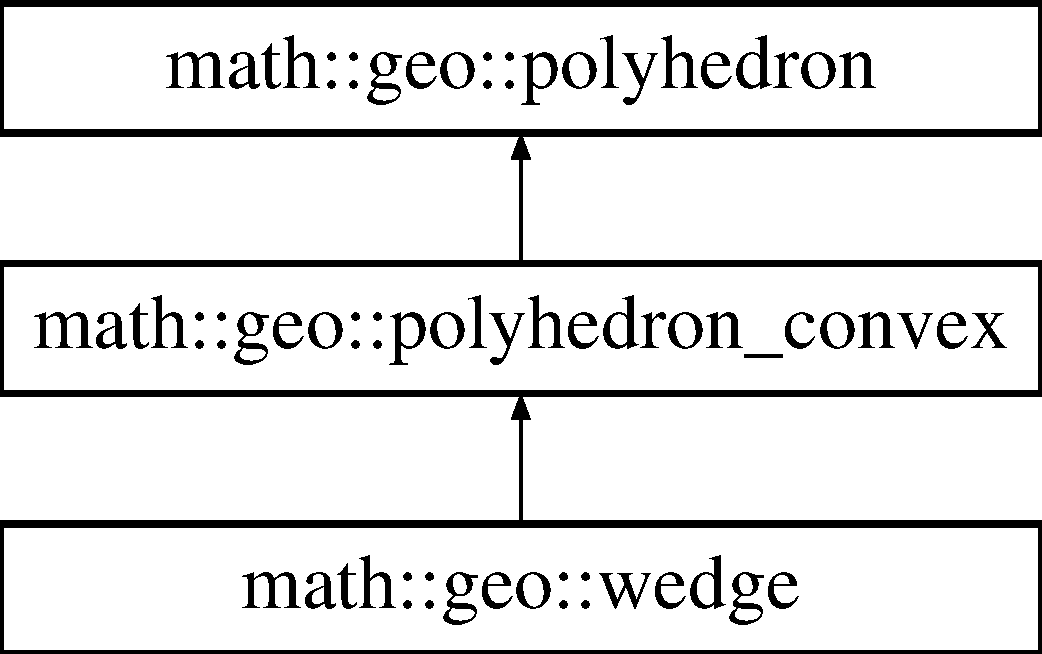
\includegraphics[height=3cm]{classmath_1_1geo_1_1wedge}
\end{center}
\end{figure}


The documentation for this class was generated from the following file:\begin{DoxyCompactItemize}
\item 
src/math/geo/polyhedron.hpp\end{DoxyCompactItemize}

\printindex
\end{document}
